% ============================================================================
% FOCUS 18: REACTION DYNAMICS
% Complete Beamer Presentation
% ============================================================================

\documentclass[aspectratio=169,12pt]{beamer}

% ============================================================================
% PACKAGES
% ============================================================================
\usepackage{amsmath}
\usepackage{amssymb}
\usepackage{chemformula}
\usepackage{siunitx}
\usepackage{tikz}
\usepackage{pgfplots}
\usepackage{qrcode}
\usepackage{hyperref}
\usepackage{booktabs}

% TikZ libraries
\usetikzlibrary{arrows.meta,positioning,shapes,decorations.pathmorphing,decorations.markings,calc}
\pgfplotsset{compat=1.18}

% ============================================================================
% THEME AND COLORS
% ============================================================================
\usetheme{Madrid}
\usecolortheme{default}

% Custom colors
\definecolor{darkblue}{RGB}{0,51,102}
\definecolor{lightblue}{RGB}{102,178,255}
\definecolor{darkred}{RGB}{153,0,0}
\definecolor{darkorange}{RGB}{204,102,0}
\definecolor{darkgreen}{RGB}{0,102,51}

\setbeamercolor{structure}{fg=darkblue}
\setbeamercolor{frametitle}{fg=white,bg=darkblue}
\setbeamercolor{title}{fg=white,bg=darkblue}
\setbeamercolor{block title}{fg=white,bg=darkblue}
\setbeamercolor{block body}{bg=lightblue!10}

% ============================================================================
% CUSTOM COMMANDS
% ============================================================================
% ============================================================================
% CUSTOM COMMANDS FOR REACTION DYNAMICS PRESENTATION
% ============================================================================

% ============================================================================
% MATHEMATICAL COMMANDS
% ============================================================================

% Differential operators
\newcommand{\diff}[1]{\mathrm{d}#1}
\newcommand{\partd}[2]{\frac{\partial #1}{\partial #2}}
\newcommand{\ddt}[1]{\frac{\diff #1}{\diff t}}

% ============================================================================
% CHEMICAL AND PHYSICAL CONSTANTS
% ============================================================================

% Boltzmann constant
\newcommand{\kB}{k_{\text{B}}}

% Avogadro's number
\newcommand{\NA}{N_{\text{A}}}

% Activation energy
\newcommand{\Ea}{E_{\text{a}}}

% Rate constants
\newcommand{\kr}{k_{\text{r}}}
\newcommand{\kd}{k_{\text{d}}}

% Quantum mechanics
\newcommand{\ket}[1]{|#1\rangle}

% ============================================================================
% THERMODYNAMIC QUANTITIES
% ============================================================================

% Gibbs energy
\newcommand{\Gibbs}{\Delta G}

% Activation parameters
\newcommand{\Hact}{\Delta^{\ddagger} H^{\circ}}
\newcommand{\Gact}{\Delta^{\ddagger} G^{\circ}}
\newcommand{\Sact}{\Delta^{\ddagger} S^{\circ}}

% ============================================================================
% SPECIAL FORMATTING
% ============================================================================

% X mark symbol for limitations/negatives
\newcommand{\xmark}{\textcolor{darkred}{\textbf{$\times$}}}

% Key equation box (highlighted equation)
\newcommand{\keyeq}[1]{%
\begin{center}
\fcolorbox{darkblue}{lightblue!20}{%
\begin{minipage}{0.85\textwidth}
\begin{equation*}
\boxed{#1}
\end{equation*}
\end{minipage}
}%
\end{center}
}

% Notebook reference with QR code
\newcommand{\notebook}[2]{%
\begin{center}
\begin{tikzpicture}
\node[rectangle,draw,fill=yellow!10,text width=0.7\textwidth,align=center,minimum height=1.5cm] (text) {%
\textbf{Interactive Notebook:} #1\\[0.2cm]
\small Scan QR code or visit: \url{#2}
};
\node[right=0.5cm of text] (qr) {\qrcode[height=1.2cm]{#2}};
\end{tikzpicture}
\end{center}
}

% Concept highlight box
\newcommand{\concept}[2]{%
\begin{block}{#1}
#2
\end{block}
}

% Emphasis box (for important points)
\newcommand{\emphbox}[1]{%
\begin{center}
\fcolorbox{darkorange}{darkorange!10}{%
\begin{minipage}{0.9\textwidth}
\centering
\textbf{#1}
\end{minipage}
}%
\end{center}
}

% ============================================================================
% ARROW STYLES FOR REACTION MECHANISMS
% ============================================================================

% Equilibrium arrow
\newcommand{\eqarrow}{\rightleftharpoons}

% Forward reaction arrow
\newcommand{\forward}{\longrightarrow}

% Reverse reaction arrow
\newcommand{\reverse}{\longleftarrow}

% ============================================================================
% UNITS (supplement siunitx if needed)
% ============================================================================

% Common unit combinations
\DeclareSIUnit\angstrom{\text{\AA}}
\DeclareSIUnit\debye{D}
\DeclareSIUnit\calorie{cal}

% ============================================================================
% COLOR DEFINITIONS FOR CONSISTENCY
% ============================================================================

% Already defined in main file, but repeated here for reference:
% \definecolor{darkblue}{RGB}{0,51,102}
% \definecolor{lightblue}{RGB}{102,178,255}
% \definecolor{darkred}{RGB}{153,0,0}
% \definecolor{darkorange}{RGB}{204,102,0}
% \definecolor{darkgreen}{RGB}{0,102,51}

% ============================================================================
% TIKZ STYLES FOR DIAGRAMS
% ============================================================================

\tikzset{
    % Molecule style
    molecule/.style={circle,draw,fill=blue!30,minimum size=0.8cm},
    % Transition state style
    transition/.style={circle,draw,fill=red!30,minimum size=0.8cm},
    % Product style
    product/.style={circle,draw,fill=green!30,minimum size=0.8cm},
    % Energy level
    level/.style={thick,blue},
    % Reaction arrow
    rxnarrow/.style={-{Stealth[length=3mm]},very thick,red}
}

% ============================================================================
% PGFPLOTS STYLES FOR CONSISTENT GRAPHS
% ============================================================================

\pgfplotsset{
    standard plot/.style={
        width=8cm,
        height=6cm,
        grid=major,
        thick,
        xlabel style={font=\small},
        ylabel style={font=\small},
        legend style={font=\footnotesize},
        tick label style={font=\footnotesize}
    }
}


% ============================================================================
% TITLE INFORMATION
% ============================================================================
\title[Focus 18: Reaction Dynamics]{Focus 18: Reaction Dynamics}
\subtitle{From Collisions to Electron Transfer}
\author{Physical Chemistry Course}
\institute{Mindanao State University -- Iligan Institute of Technology}
\date{\today}

% ============================================================================
% DOCUMENT
% ============================================================================
\begin{document}

% Title slide
\begin{frame}
\titlepage
\end{frame}

% Table of contents
\begin{frame}{Outline}
\tableofcontents
\end{frame}

% ============================================================================
% INTRODUCTION
% ============================================================================
\section{Introduction}

\begin{frame}{What is Reaction Dynamics?}

\textbf{Reaction Dynamics} studies the \alert{detailed molecular mechanisms} of chemical reactions

\vspace{0.3cm}

\begin{columns}[T]

\column{0.5\textwidth}

\textbf{Beyond traditional kinetics:}

\begin{itemize}
\item How do molecules collide?
\item What happens during collision?
\item Where does energy go?
\item What is the reaction path?
\item How fast can reactions be?
\end{itemize}

\vspace{0.3cm}

\textbf{Time scales:}
\begin{itemize}
\item Bond vibrations: fs ($10^{-15}$ s)
\item Reactions: ps-ns ($10^{-12}$-$10^{-9}$ s)
\item Diffusion: ns-$\mu$s
\end{itemize}

\column{0.5\textwidth}

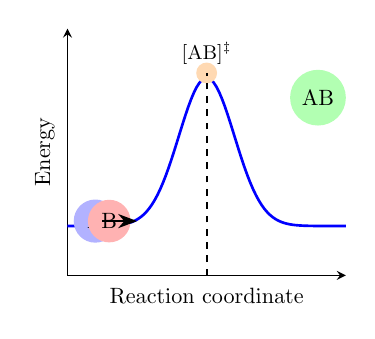
\begin{tikzpicture}[scale=0.8]
% Simple reaction coordinate diagram
\begin{axis}[
    width=6cm,
    height=5.5cm,
    xlabel={Reaction coordinate},
    ylabel={Energy},
    xmin=0, xmax=10,
    ymin=0, ymax=100,
    grid=none,
    axis lines=left,
    xtick=\empty,
    ytick=\empty,
    thick
]

% Energy profile
\addplot[blue,very thick,domain=0:10,samples=100] {
    20 + 60*exp(-((x-5)^2)/2)
};

% Reactants
\node[circle,fill=blue!30] at (axis cs:1,22) {A};
\node[circle,fill=red!30] at (axis cs:1.5,22) {B};
\draw[-{Stealth[length=3mm]},thick] (axis cs:1.25,22) -- (axis cs:2.5,22);

% Transition state
\node[circle,fill=orange!30] at (axis cs:5,82) {};
\draw[dashed] (axis cs:5,0) -- (axis cs:5,82);
\node[above,font=\small] at (axis cs:5,82) {[\ch{AB}]$^{\ddagger}$};

% Products
\node[circle,fill=green!30] at (axis cs:9,72) {AB};

\end{axis}
\end{tikzpicture}

\end{columns}

\end{frame}

\begin{frame}{The Journey Through Focus 18}

\vspace{-0.5cm}
\begin{center}
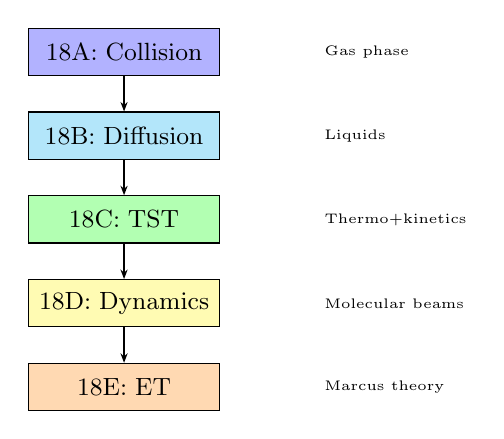
\begin{tikzpicture}[
    node distance=0.45cm,
    topic/.style={rectangle,draw,fill=blue!20,text width=2.2cm,align=center,minimum height=0.6cm,font=\footnotesize},
    arrow/.style={-{Stealth[length=1.2mm]},thick}
]

% Topics
\node[topic,fill=blue!30] (18A) {\small 18A: Collision};
\node[topic,fill=cyan!30,below=of 18A] (18B) {\small 18B: Diffusion};
\node[topic,fill=green!30,below=of 18B] (18C) {\small 18C: TST};
\node[topic,fill=yellow!30,below=of 18C] (18D) {\small 18D: Dynamics};
\node[topic,fill=orange!30,below=of 18D] (18E) {\small 18E: ET};

% Arrows
\draw[arrow] (18A) -- (18B);
\draw[arrow] (18B) -- (18C);
\draw[arrow] (18C) -- (18D);
\draw[arrow] (18D) -- (18E);

% Compact side annotations
\node[right=1.2cm of 18A,font=\tiny] {Gas phase};
\node[right=1.2cm of 18B,font=\tiny] {Liquids};
\node[right=1.2cm of 18C,font=\tiny] {Thermo+kinetics};
\node[right=1.2cm of 18D,font=\tiny] {Molecular beams};
\node[right=1.2cm of 18E,font=\tiny] {Marcus theory};

\end{tikzpicture}
\end{center}

\end{frame}

\begin{frame}{Learning Objectives}

By the end of this topic, you should be able to:

\begin{enumerate}
\item Calculate collision frequencies and reaction cross-sections from molecular properties

\item Distinguish between diffusion-controlled and activation-controlled reactions

\item Apply transition-state theory to calculate rate constants from thermodynamic parameters

\item Interpret kinetic isotope effects and quantum tunneling in chemical reactions

\item Analyze molecular beam experiments and potential energy surfaces

\item Apply Marcus theory to electron transfer reactions and predict rates
\end{enumerate}

\end{frame}

\begin{frame}{Prerequisites - Quick Reminder}

\textbf{From earlier topics, you should know:}

\vspace{0.3cm}

\begin{columns}[T]

\column{0.5\textwidth}

\textbf{Kinetic Theory:}
\begin{itemize}
\item Maxwell-Boltzmann distribution
\item Mean speeds: $\bar{v} = \sqrt{8kT/\pi m}$
\item Collision frequency
\end{itemize}

\vspace{0.2cm}

\textbf{Chemical Kinetics:}
\begin{itemize}
\item Rate laws and rate constants
\item Arrhenius equation: $k = Ae^{-E_a/RT}$
\item Reaction mechanisms
\end{itemize}

\column{0.5\textwidth}

\textbf{Thermodynamics:}
\begin{itemize}
\item Gibbs energy: $\Delta G = \Delta H - T\Delta S$
\item Equilibrium constants
\item Standard states
\end{itemize}

\vspace{0.2cm}

\textbf{Statistical Mechanics:}
\begin{itemize}
\item Partition functions
\item Boltzmann distribution
\item Energy levels
\end{itemize}

\end{columns}

\end{frame}

% ============================================================================
% INCLUDE TOPIC FILES
% ============================================================================
% ============================================================================
% TOPIC 18A: COLLISION THEORY
% ============================================================================

\section{Topic 18A: Collision Theory}

% ===========================================================================
% Slide 6: Topic 18A Overview
% ===========================================================================
\begin{frame}{Topic 18A: Collision Theory}

\begin{columns}[T]

\column{0.5\textwidth}
\textbf{The Simplest Model:}

\vspace{0.2cm}

Reactions occur when molecules collide \textit{if}:

\begin{enumerate}
\item They collide with sufficient frequency
\item They have enough kinetic energy ($\ge E_a$)
\item They have correct orientation (steric factor)
\end{enumerate}

\vspace{0.2cm}

\textbf{Learning Objectives:}
\begin{itemize}
\item Derive collision rate from kinetic theory
\item Connect to Arrhenius equation
\item Understand steric factors
\item Apply to unimolecular reactions
\end{itemize}

\column{0.5\textwidth}
\centering

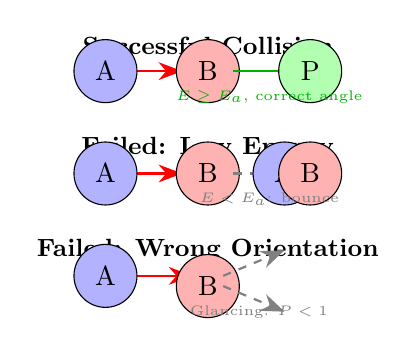
\begin{tikzpicture}[scale=0.65]
% Successful collision
\node[font=\small] at (0,3.5) {\textbf{Successful Collision}};
\draw[-{Stealth[length=3mm]},thick,red] (-2,3) -- (-0.5,3);
\node[circle,draw,fill=blue!30,minimum size=0.8cm] at (-2,3) {A};
\node[circle,draw,fill=red!30,minimum size=0.8cm] at (0,3) {B};
\draw[-{Stealth[length=3mm]},thick,green!70!black] (0.5,3) -- (2,3);
\node[circle,draw,fill=green!30,minimum size=0.8cm] at (2,3) {P};
\node[font=\tiny,text=green!70!black] at (1.2,2.5) {$E \ge E_a$, correct angle};

% Failed collision - not enough energy
\node[font=\small] at (0,1.5) {\textbf{Failed: Low Energy}};
\draw[-{Stealth[length=3mm]},thick,red] (-2,1) -- (-0.5,1);
\node[circle,draw,fill=blue!30,minimum size=0.8cm] at (-2,1) {A};
\node[circle,draw,fill=red!30,minimum size=0.8cm] at (0,1) {B};
\draw[-{Stealth[length=3mm]},thick,gray,dashed] (0.5,1) -- (2,1);
\node[circle,draw,fill=blue!30,minimum size=0.8cm] at (1.5,1) {A};
\node[circle,draw,fill=red!30,minimum size=0.8cm] at (2,1) {B};
\node[font=\tiny,text=gray] at (1.2,0.5) {$E < E_a$: bounce};

% Failed collision - wrong orientation
\node[font=\small] at (0,-0.5) {\textbf{Failed: Wrong Orientation}};
\draw[-{Stealth[length=3mm]},thick,red] (-2,-1) -- (-0.3,-1);
\node[circle,draw,fill=blue!30,minimum size=0.8cm] at (-2,-1) {A};
\node[circle,draw,fill=red!30,minimum size=0.8cm] at (0,-1.2) {B};
\draw[-{Stealth[length=3mm]},thick,gray,dashed] (0.3,-1) -- (1.5,-0.5);
\draw[-{Stealth[length=3mm]},thick,gray,dashed] (0.3,-1.2) -- (1.5,-1.7);
\node[font=\tiny,text=gray] at (1,-1.7) {Glancing: $P < 1$};
\end{tikzpicture}

\end{columns}

\end{frame}

% ===========================================================================
% Slide: Kinetic Molecular Theory Background
% ===========================================================================
\begin{frame}{Kinetic Molecular Theory Background}

\textbf{Maxwell-Boltzmann Distribution of Speeds:}

The fraction of molecules with speeds between $v$ and $v + dv$:

\[ f(v) = 4\pi \left(\frac{m}{2\pi \kB T}\right)^{3/2} v^2 e^{-mv^2/2\kB T} \]

\begin{columns}[T]
\column{0.5\textwidth}
\textbf{Key Quantities:}
\begin{itemize}
\item Mean speed: $\bar{v} = \left(\frac{8\kB T}{\pi m}\right)^{1/2}$
\item Root-mean-square: $v_{rms} = \left(\frac{3\kB T}{m}\right)^{1/2}$
\item Most probable: $v_p = \left(\frac{2\kB T}{m}\right)^{1/2}$
\end{itemize}

\column{0.5\textwidth}
\centering
\includegraphics[width=\textwidth]{Reaction_Dynamics_Interactive/images/maxwell_boltzmann_speeds.png}

\vspace{0.2cm}
\tiny \textit{Interactive version: Scan QR code at end of topic}
\end{columns}

\end{frame}

% ===========================================================================
% Slide: Collision Cross-Section - Detailed
% ===========================================================================
\begin{frame}{Collision Cross-Section - Hard Sphere Model}

\begin{columns}[T]
\column{0.5\textwidth}
\textbf{Geometric Definition:}
\begin{itemize}
\item Treat molecules as hard spheres
\item Radii $r_A$ and $r_B$
\item Collision occurs when centers approach within $d = r_A + r_B$
\item Target area: $\sigma = \pi d^2$
\end{itemize}

\vspace{0.2cm}
\keyeq{\sigma = \pi d^2 = \pi (r_A + r_B)^2}

\textbf{Impact Parameter $b$:}
\begin{itemize}
\item Perpendicular distance between trajectories
\item Collision if $b \le d$
\end{itemize}

\column{0.5\textwidth}
\centering
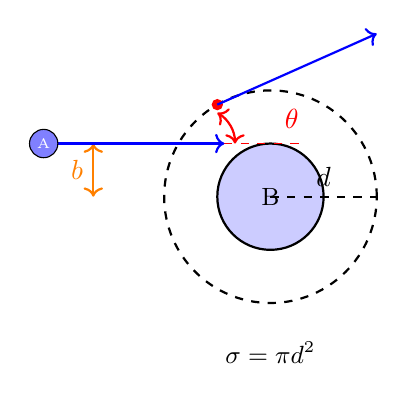
\begin{tikzpicture}[scale=0.9]
    % Target molecule (center)
    \draw[fill=blue!20, thick] (0,0) circle (0.75cm);
    \node at (0,0) {\small B};

    % Collision diameter
    \draw[dashed, thick] (0,0) circle (1.5cm);
    \draw[dashed, thick] (0,0) -- (1.5,0) node[midway, above] {$d$};

    % Impact parameter b = 0.75 cm
    \draw[red, dashed] (-3, 0.75) -- (0.5, 0.75);
    \draw[<->, orange, thick] (-2.5, 0) -- (-2.5, 0.75) node[midway, left] {$b$};

    % Projectile molecule A trajectory
    % Incoming straight line
    \draw[->, thick, blue] (-3.2, 0.75) -- (-0.65, 0.75);
    \draw[fill=blue!50] (-3.2, 0.75) circle (0.2cm) node[white] {\tiny A};

    % Contact point at angle θ from center
    \coordinate (contact) at ({-1.5*0.5},{1.5*0.866}); % at 120 degrees
    \fill[red] (contact) circle (0.08cm);

    % Outgoing deflected trajectory
    \draw[->, thick, blue] (contact) -- (1.5, 2.3);

    % Scattering angle
    \draw[<->, red, thick] (-0.5, 0.75) arc[start angle=0, end angle=60, radius=0.5cm];
    \node[red] at (0.3, 1.1) {$\theta$};

    % Label
    \node at (0,-2.2) {\small $\sigma = \pi d^2$};
\end{tikzpicture}
\end{columns}

\vspace{0.2cm}
\textbf{Typical Values:} $d \approx 0.3-0.5$ nm, $\sigma \approx 0.1-1$ nm$^2$ (10-100 \AA$^2$)

\end{frame}

% ===========================================================================
% Slide: Derivation of Collision Rate - Part 1
% ===========================================================================
\begin{frame}{Derivation of Collision Rate (Part 1)}

\textbf{Setup:} Consider molecule A moving through gas of B molecules.

\vspace{0.3cm}

\textbf{Step 1: Collision Cylinder}
\begin{itemize}
\item In time $\Delta t$, A sweeps volume $V = \sigma v_{rel} \Delta t$
\item Number of B molecules in cylinder: $N_B = \mathcal{N}_B \cdot \sigma v_{rel} \Delta t$
\item Collision rate for one A: $\sigma v_{rel} \mathcal{N}_B$
\end{itemize}

\vspace{0.3cm}

\textbf{Step 2: Average Over Velocity Distribution}
\begin{itemize}
\item Must average over Maxwell-Boltzmann distribution of $v_{rel}$
\item For two species: $\bar{v}_{rel} = \left(\frac{8\kB T}{\pi \mu}\right)^{1/2}$
\item Reduced mass: $\mu = \frac{m_A m_B}{m_A + m_B}$
\end{itemize}

\end{frame}

% ===========================================================================
% Slide: Derivation of Collision Rate - Part 2
% ===========================================================================
\begin{frame}{Derivation of Collision Rate (Part 2)}

\textbf{Step 3: Total Collision Density}

Total collisions per unit volume per unit time between A and B molecules:

\vspace{0.5cm}

\keyeq{Z_{AB} = \sigma \left(\frac{8\kB T}{\pi \mu}\right)^{1/2} \mathcal{N}_A \mathcal{N}_B}

\vspace{0.5cm}

\textbf{Physical Interpretation:}
\begin{itemize}
\item $\sigma$ = collision cross-section (geometric factor)
\item $\bar{v}_{rel} = \left(\frac{8\kB T}{\pi \mu}\right)^{1/2}$ = mean relative speed
\item $\mathcal{N}_A$, $\mathcal{N}_B$ = number densities (molecules per unit volume)
\item $Z_{AB}$ has units: collisions m$^{-3}$ s$^{-1}$
\end{itemize}

\end{frame}

% ===========================================================================
% Slide: Collision Rate - Identical Molecules
% ===========================================================================
\begin{frame}{Special Case: Identical Molecules}

For collisions between identical molecules A + A:

\vspace{0.2cm}

\textbf{Modified Formula:}
\begin{itemize}
\item Must avoid double-counting (each collision counted twice)
\item Factor of $1/2$ correction
\end{itemize}

\keyeq{Z_{AA} = \frac{1}{2} \sigma \left(\frac{8\kB T}{\pi \mu}\right)^{1/2} \mathcal{N}_A^2}

\vspace{0.2cm}

\textbf{For identical molecules:}
\begin{itemize}
\item $\mu = m_A/2$ (reduced mass)
\item $\bar{v}_{rel} = \sqrt{2} \bar{v}$ where $\bar{v}$ is mean speed of one molecule
\item Collision frequency is $\sqrt{2}$ times what you'd naively expect
\end{itemize}

\end{frame}

% ===========================================================================
% Slide: Worked Example - Collision Density Part 1
% ===========================================================================
\begin{frame}{Worked Example: Collision Rate for N$_2$ (Part 1)}

\textbf{Problem:} Calculate $Z_{N_2-N_2}$ for nitrogen gas at 298 K and 1 bar.
Given: $\sigma \approx 0.43$ nm$^2$ = $4.3 \times 10^{-19}$ m$^2$

\vspace{0.3cm}

\textbf{Step 1: Number density from ideal gas law}
\[ \mathcal{N} = \frac{P}{\kB T} = \frac{10^5 \text{ Pa}}{(1.381 \times 10^{-23} \text{ J K}^{-1})(298 \text{ K})} = 2.43 \times 10^{25} \text{ m}^{-3} \]

\vspace{0.3cm}

\textbf{Step 2: Mean relative speed}

Mass of N$_2$: $m = 28$ amu $= 4.65 \times 10^{-26}$ kg

Reduced mass: $\mu = m/2 = 2.32 \times 10^{-26}$ kg

\[ \bar{v}_{rel} = \sqrt{\frac{8 \times 1.381 \times 10^{-23} \times 298}{\pi \times 2.32 \times 10^{-26}}} = 670 \text{ m s}^{-1} \]

\end{frame}

% ===========================================================================
% Slide: Worked Example - Collision Density Part 2
% ===========================================================================
\begin{frame}{Worked Example: Collision Rate for N$_2$ (Part 2)}

\textbf{Step 3: Calculate collision density}

Using the formula: $Z_{N_2-N_2} = \frac{1}{2} \sigma \bar{v}_{rel} \mathcal{N}^2$

\vspace{0.3cm}

\[ Z_{N_2-N_2} = \frac{1}{2} \times 4.3 \times 10^{-19} \times 670 \times (2.43 \times 10^{25})^2 \]

\vspace{0.3cm}

\[ \boxed{Z_{N_2-N_2} \approx 5 \times 10^{34} \text{ collisions m}^{-3} \text{ s}^{-1}} \]

\vspace{0.3cm}

\textbf{Interpretation:} This enormous collision rate shows why most gas reactions require activation energy - if every collision reacted, all reactions would be instantaneous!

\end{frame}

% ===========================================================================
% Slide: Energy Requirements - Boltzmann Factor
% ===========================================================================
\begin{frame}{Energy Requirements: Not All Collisions React}

\textbf{The Problem:}
\begin{itemize}
\item $Z_{AB} \sim 10^{34}$ collisions m$^{-3}$ s$^{-1}$ is enormous!
\item If every collision led to reaction, all reactions would be over in nanoseconds
\item Reality: Most reactions have measurable rates (seconds to hours)
\end{itemize}

\vspace{0.3cm}

\textbf{The Solution: Activation Energy}
\begin{itemize}
\item Only collisions with kinetic energy $\varepsilon \ge E_a$ along line of centers react
\item Fraction of molecules with energy $> E_a$ from Boltzmann distribution:
\end{itemize}

\keyeq{f(E > E_a) = \int_{E_a}^{\infty} f(E) dE = e^{-E_a/RT}}

\vspace{0.2cm}
\emphbox{The exponential factor dramatically reduces the reactive collision rate}

\end{frame}

% ===========================================================================
% Slide: Energy Distribution
% ===========================================================================
\begin{frame}{Maxwell-Boltzmann Energy Distribution}

The fraction of molecules with translational energy between $\varepsilon$ and $\varepsilon + d\varepsilon$:

\[ f(\varepsilon) = \frac{2\pi}{(\pi \kB T)^{3/2}} \varepsilon^{1/2} e^{-\varepsilon/\kB T} \]

\begin{columns}[T]
\column{0.5\textwidth}
\textbf{Key Features:}
\begin{itemize}
\item Maximum at $\varepsilon = \kB T/2$
\item Mean energy: $\langle \varepsilon \rangle = \frac{3}{2}\kB T$
\item High-energy tail decays exponentially
\item Fraction with $\varepsilon > E_a$: \[\int_{E_a}^{\infty} f(\varepsilon) d\varepsilon = e^{-E_a/\kB T}\]
\end{itemize}

\column{0.5\textwidth}
\centering
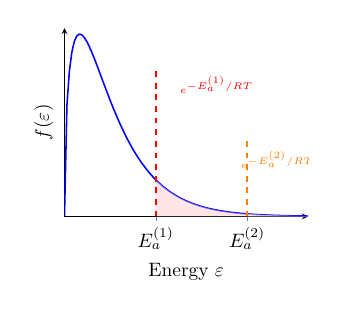
\begin{tikzpicture}[scale=0.7]
\begin{axis}[
    xlabel={Energy $\varepsilon$},
    ylabel={$f(\varepsilon)$},
    axis lines=left,
    xmin=0, xmax=8,
    ymin=0, ymax=0.5,
    xtick={3,6},
    xticklabels={$E_a^{(1)}$, $E_a^{(2)}$},
    ytick=\empty,
    width=6cm,
    height=5cm
]
% Correct Maxwell-Boltzmann energy distribution: f(ε) = (2/√π)√ε exp(-ε)
\addplot[blue, thick, domain=0:8, samples=100] {2/sqrt(pi)*sqrt(x)*exp(-x)};
\addplot[fill=red!20, draw=none, opacity=0.5, domain=3:8, samples=50] {2/sqrt(pi)*sqrt(x)*exp(-x)} \closedcycle;
\addplot[fill=orange!20, draw=none, opacity=0.5, domain=6:8, samples=30] {2/sqrt(pi)*sqrt(x)*exp(-x)} \closedcycle;
\draw[red, dashed, thick] (axis cs:3,0) -- (axis cs:3,0.4);
\draw[orange, dashed, thick] (axis cs:6,0) -- (axis cs:6,0.2);
\node[red] at (axis cs:5,0.35) {\tiny $e^{-E_a^{(1)}/RT}$};
\node[orange] at (axis cs:7,0.15) {\tiny $e^{-E_a^{(2)}/RT}$};
\end{axis}
\end{tikzpicture}
\end{columns}

\textbf{Higher $E_a$ $\Rightarrow$ Smaller reactive fraction $\Rightarrow$ Slower reaction}

\end{frame}

% ===========================================================================
% Slide: Energy-Dependent Cross-Section
% ===========================================================================
\begin{frame}{Reactive Cross-Section: Energy Dependence}

The collision cross-section depends on collision energy $\varepsilon$:

\keyeq{\sigma_r(\varepsilon) = \begin{cases}
0 & \varepsilon < E_a \\
\sigma \left(1 - \frac{E_a}{\varepsilon}\right) & \varepsilon \ge E_a
\end{cases}}

\begin{columns}[T]
\column{0.55\textwidth}
\textbf{Physical Interpretation:}
\begin{itemize}
\item Below $E_a$: No reaction possible ($\sigma_r = 0$)
\item At $E_a$: Reaction just becomes possible ($\sigma_r = 0$)
\item Well above $E_a$: Approaches geometric $\sigma$
\item The factor $(1 - E_a/\varepsilon)$ represents the "likelihood" of having enough energy in the right direction
\end{itemize}

\column{0.45\textwidth}
\centering
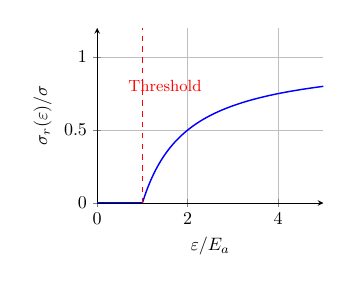
\begin{tikzpicture}[scale=0.65]
\begin{axis}[
    xlabel={$\varepsilon/E_a$},
    ylabel={$\sigma_r(\varepsilon)/\sigma$},
    xmin=0, xmax=5,
    ymin=0, ymax=1.2,
    axis lines=left,
    grid=major,
    width=6cm,
    height=5cm
]
\addplot[blue, thick, domain=1:5, samples=100] {1 - 1/x};
\addplot[blue, thick, domain=0:1, samples=2] {0};
\draw[red, dashed] (axis cs:1,0) -- (axis cs:1,1.2);
\node[red] at (axis cs:1.5,0.8) {\small Threshold};
\end{axis}
\end{tikzpicture}

\vspace{0.2cm}
\small The linear rise from threshold is a simplified model; real reactions may have different energy dependencies.
\end{columns}

\end{frame}

% ===========================================================================
% Slide: Derivation of Rate Constant
% ===========================================================================
\begin{frame}{Derivation of the Collision Theory Rate Constant}

\textbf{Starting Point:} Reactive collision rate per unit volume

\[ \text{Rate} = \int_0^{\infty} \sigma_r(\varepsilon) v_{rel}(\varepsilon) \mathcal{N}_A \mathcal{N}_B f(\varepsilon) d\varepsilon \]

\textbf{Key Steps:}
\begin{enumerate}
\item Insert $\sigma_r(\varepsilon) = \sigma(1 - E_a/\varepsilon)$ for $\varepsilon \ge E_a$
\item Use $v_{rel} = \sqrt{2\varepsilon/\mu}$ (relation between speed and energy)
\item Integrate over Boltzmann distribution $f(\varepsilon) \propto e^{-\varepsilon/\kB T}$
\end{enumerate}

\vspace{0.2cm}

\textbf{Result after integration:}

\keyeq{k_r = \NA \sigma \left(\frac{8\kB T}{\pi \mu}\right)^{1/2} e^{-E_a/RT}}

\vspace{0.2cm}

\textbf{In terms of molar concentrations $[A]$, $[B]$:}
\[ \text{Rate} = k_r [A][B] \]

\end{frame}

% ===========================================================================
% Slide: Connection to Arrhenius Equation
% ===========================================================================
\begin{frame}{Connection to Arrhenius Equation}

\textbf{Collision Theory Result:}
\[ k_r = \NA \sigma \left(\frac{8\kB T}{\pi \mu}\right)^{1/2} e^{-E_a/RT} \]

\textbf{Arrhenius Empirical Form:}
\[ k = A e^{-E_a/RT} \]

\vspace{0.3cm}

\textbf{Identification of Pre-exponential Factor:}
\keyeq{A_{theory} = \NA \sigma \left(\frac{8\kB T}{\pi \mu}\right)^{1/2}}

\begin{itemize}
\item Typical values: $A \sim 10^{10} - 10^{11}$ dm$^3$ mol$^{-1}$ s$^{-1}$ for bimolecular gas reactions
\item Temperature dependence: $A \propto T^{1/2}$ (weak, often ignored)
\item For Arrhenius plots ($\ln k$ vs $1/T$): slope = $-E_a/R$, intercept = $\ln A$
\end{itemize}

\end{frame}

% ===========================================================================
% Slide: Numerical Example of A-factor Part 1
% ===========================================================================
\begin{frame}{Numerical Calculation of $A$-factor (Part 1)}

\textbf{Example:} Calculate $A$ for H$_2$ + I$_2 \to$ 2HI at 600 K

\vspace{0.2cm}

\textbf{Given:}
\begin{itemize}
\item $\sigma = 0.30$ nm$^2$ = $3.0 \times 10^{-19}$ m$^2$
\item $m_{H_2} = 2.016$ amu = $3.35 \times 10^{-27}$ kg
\item $m_{I_2} = 253.8$ amu = $4.22 \times 10^{-25}$ kg
\end{itemize}

\vspace{0.3cm}

\textbf{Step 1: Reduced mass}
\[ \mu = \frac{m_{H_2} \cdot m_{I_2}}{m_{H_2} + m_{I_2}} = \frac{3.35 \times 10^{-27} \times 4.22 \times 10^{-25}}{4.25 \times 10^{-25}} = 3.32 \times 10^{-27} \text{ kg} \]

\vspace{0.3cm}

\textbf{Step 2: Mean relative speed}
\[ \bar{v}_{rel} = \sqrt{\frac{8 \times 1.381 \times 10^{-23} \times 600}{3.14159 \times 3.32 \times 10^{-27}}} = 2520 \text{ m s}^{-1} \]

\end{frame}

% ===========================================================================
% Slide: Numerical Example of A-factor Part 2
% ===========================================================================
\begin{frame}{Numerical Calculation of $A$-factor (Part 2)}

\textbf{Step 3: Calculate A-factor}

Using the formula: $A = \NA \sigma \bar{v}_{rel}$

\vspace{0.2cm}

\[ A = 6.022 \times 10^{23} \times 3.0 \times 10^{-19} \times 2520 \]

\[ A = 4.6 \times 10^8 \text{ m}^3 \text{ mol}^{-1} \text{ s}^{-1} \]

\vspace{0.2cm}

Converting to dm$^3$ (multiply by $10^3$):

\[ \boxed{A = 4.6 \times 10^{11} \text{ dm}^3 \text{ mol}^{-1} \text{ s}^{-1}} \]

\vspace{0.15cm}

\textbf{Interpretation:} This is in the typical range $10^{10}-10^{11}$ for bimolecular gas reactions, consistent with collision theory predictions!

\end{frame}

% ===========================================================================
% Slide: The Steric Factor Problem
% ===========================================================================
\begin{frame}{The Steric Factor Problem}

\textbf{Experiment vs Theory:} Does $A_{exp}$ match $A_{theory}$?

\vspace{0.2cm}

\begin{table}
\centering
\small
\begin{tabular}{lccc}
\toprule
\textbf{Reaction} & $\mathbf{A_{exp}}$ & $\mathbf{A_{theory}}$ & $\mathbf{P = A_{exp}/A_{theory}}$ \\
 & (dm$^3$ mol$^{-1}$ s$^{-1}$) & (dm$^3$ mol$^{-1}$ s$^{-1}$) & \\
\midrule
2NOCl $\to$ 2NO + Cl$_2$ & $9.4 \times 10^9$ & $5.9 \times 10^{10}$ & 0.16 \\
2ClO $\to$ Cl$_2$ + O$_2$ & $6.3 \times 10^7$ & $2.5 \times 10^{10}$ & 0.0025 \\
H$_2$ + C$_2$H$_4 \to$ C$_2$H$_6$ & $1.2 \times 10^6$ & $7.3 \times 10^{10}$ & $1.7 \times 10^{-5}$ \\
K + Br$_2 \to$ KBr + Br & $1.0 \times 10^{12}$ & $2.1 \times 10^{11}$ & \alert{4.8} \\
\bottomrule
\end{tabular}
\end{table}

\vspace{0.3cm}

\textbf{Observations:}
\begin{itemize}
\item \textbf{Usually $P < 1$:} Not all orientations are reactive (steric hindrance)
\item \textbf{Complex molecules:} Smaller $P$ (need precise alignment)
\item \textbf{Sometimes $P > 1$:} Long-range forces extend reactive range (Harpoon mechanism)
\end{itemize}

\end{frame}

% ===========================================================================
% Slide: Steric Factor - Physical Basis Part 1
% ===========================================================================
\begin{frame}{The Steric Factor: Modified Collision Theory}

\textbf{Modified Collision Theory:}

\keyeq{k_r = P \cdot \NA \sigma \left(\frac{8\kB T}{\pi \mu}\right)^{1/2} e^{-E_a/RT}}

\vspace{0.15cm}

\textbf{What is P?}
\begin{itemize}
\item \textbf{Steric factor:} Fraction of collisions with proper orientation
\item Effective reactive cross-section: $\sigma_r = P \sigma$
\item Depends on molecular geometry and reaction mechanism
\item Accounts for orientation requirements
\end{itemize}

\vspace{0.15cm}

\textbf{Examples:}
\begin{itemize}
\item \textbf{Atoms:} $P \approx 1$ (spherically symmetric)
\item \textbf{Linear molecules:} $P \sim 0.1-1$ (need end-on approach)
\item \textbf{Complex molecules:} $P \sim 10^{-6}-10^{-2}$ (specific reactive site)
\end{itemize}

\end{frame}

% ===========================================================================
% Slide: Steric Factor - Reactive Geometry
% ===========================================================================
\begin{frame}{The Steric Factor: Reactive Geometry}

\begin{columns}[T]
\column{0.5\textwidth}
\textbf{Orientation Matters:}

\vspace{0.1cm}

Only certain collision geometries lead to reaction:
\begin{itemize}
\item \textcolor{green!70!black}{\textbf{Reactive:}} Attack at reactive site
\item \textcolor{red}{\textbf{Non-reactive:}} Wrong orientation or glancing collision
\end{itemize}

\vspace{0.15cm}

The steric factor $P$ quantifies the fraction of properly oriented collisions.

\column{0.5\textwidth}
\centering
\textbf{Reactive Geometry:}

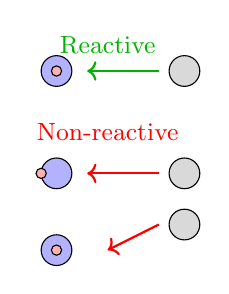
\begin{tikzpicture}[scale=0.65]
% Reactive approach
\node at (0,2.5) {\small \textcolor{green!70!black}{Reactive}};
\draw[fill=blue!30] (-1,2) circle (0.3cm);
\draw[fill=red!30] (-1,2) circle (0.1cm);
\draw[->, thick, green!70!black] (1,2) -- (-0.4,2);
\draw[fill=gray!30] (1.5,2) circle (0.3cm);

% Non-reactive approach 1
\node at (0,0.8) {\small \textcolor{red}{Non-reactive}};
\draw[fill=blue!30] (-1,0) circle (0.3cm);
\draw[fill=red!30] (-1.3,0) circle (0.1cm);
\draw[->, thick, red] (1,0) -- (-0.4,0);
\draw[fill=gray!30] (1.5,0) circle (0.3cm);

% Non-reactive approach 2
\draw[fill=blue!30] (-1,-1.5) circle (0.3cm);
\draw[fill=red!30] (-1,-1.5) circle (0.1cm);
\draw[->, thick, red] (1,-1) -- (0,-1.5);
\draw[fill=gray!30] (1.5,-1) circle (0.3cm);
\end{tikzpicture}

\vspace{0.1cm}
\small Red dot = reactive site
\end{columns}

\end{frame}

% ===========================================================================
% Slide: Case Study - Harpoon Mechanism Part 1
% ===========================================================================
\begin{frame}{Case Study: The Harpoon Mechanism ($P > 1$)}

\textbf{Reaction:} K + Br$_2 \to$ KBr + Br \quad ($P \approx 4.8$!)

\vspace{0.3cm}

\textbf{Why does $P > 1$?} Long-range electron transfer!

\vspace{0.2cm}

\textbf{Mechanism:}
\begin{enumerate}
\item K has low ionization energy ($I_K = 4.34$ eV)
\item Br$_2$ has high electron affinity ($E_{ea} = 2.55$ eV)
\item At critical distance $R^*$, electron transfer becomes favorable:
\[ K + Br_2 \to K^+ + Br_2^- \]
\item Coulombic attraction pulls ions together (like throwing a harpoon!)
\item $R^* \gg d$ (geometric), so $\sigma_{reactive} > \sigma_{geometric}$
\end{enumerate}

\vspace{0.2cm}

\textbf{Estimate of $R^*$:}
\[ I_K - E_{ea} = \frac{e^2}{4\pi\varepsilon_0 R^*} \]
\[ R^* \approx 0.8 \text{ nm} \quad (\text{vs } d \approx 0.3 \text{ nm}) \]

\end{frame}

% ===========================================================================
% Slide: Case Study - Harpoon Mechanism Part 2
% ===========================================================================
\begin{frame}{The Harpoon Mechanism: Visualization}

\begin{columns}[T]
\column{0.5\textwidth}
\textbf{Three-Step Process:}

\vspace{0.2cm}

\textbf{(1) Approach:} K and Br$_2$ approach as neutrals

\vspace{0.3cm}

\textbf{(2) Electron Jump:} At $R^*$, electron transfers to Br$_2$

\vspace{0.3cm}

\textbf{(3) Harpoon:} Coulombic attraction pulls ions together

\vspace{0.3cm}

\emphbox{Reactive cross-section much larger than geometric!}

\column{0.5\textwidth}
\centering
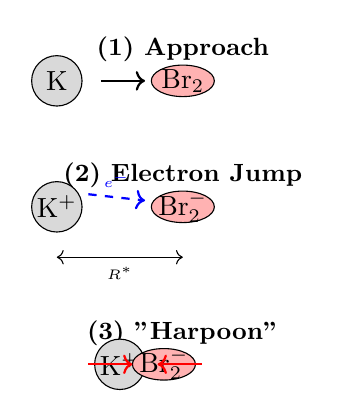
\begin{tikzpicture}[scale=0.8]
% Initial state
\node at (0,3) {\small \textbf{(1) Approach}};
\draw[fill=gray!30] (-2,2.5) circle (0.4cm) node {K};
\draw[fill=red!30] (0,2.5) ellipse (0.5cm and 0.25cm) node {Br$_2$};
\draw[->, thick] (-1.3,2.5) -- (-0.6,2.5);

% Electron transfer
\node at (0,1) {\small \textbf{(2) Electron Jump}};
\draw[fill=gray!30] (-2,0.5) circle (0.4cm) node {K$^+$};
\draw[fill=red!30] (0,0.5) ellipse (0.5cm and 0.25cm) node {Br$_2^-$};
\draw[->, dashed, thick, blue] (-1.5,0.7) -- (-0.6,0.6) node[midway, above] {\tiny $e^-$};
\draw[<->] (-2,-0.3) -- (0,-0.3) node[midway, below] {\tiny $R^*$};

% Attraction
\node at (0,-1.5) {\small \textbf{(3) "Harpoon"}};
\draw[fill=gray!30] (-1,-2) circle (0.4cm) node {K$^+$};
\draw[fill=red!30] (-0.3,-2) ellipse (0.5cm and 0.25cm) node {Br$_2^-$};
\draw[->, thick, red] (-1.5,-2) -- (-0.8,-2);
\draw[->, thick, red] (0.3,-2) -- (-0.4,-2);
\end{tikzpicture}
\end{columns}

\end{frame}

% ===========================================================================
% Slide: Temperature Dependence
% ===========================================================================
\begin{frame}{Temperature Dependence of Reaction Rates}

From collision theory: $k = A T^{1/2} e^{-E_a/RT}$

\vspace{0.2cm}

\textbf{Taking logarithm:}
\[ \ln k = \ln A + \frac{1}{2}\ln T - \frac{E_a}{RT} \]

\textbf{Arrhenius plot} ($\ln k$ vs $1/T$) assumes $A$ is constant:
\[ \ln k = \ln A - \frac{E_a}{RT} \]

\begin{columns}[T]
\column{0.5\textwidth}
\textbf{In practice:}
\begin{itemize}
\item The $T^{1/2}$ factor is weak
\item Over typical experimental ranges (50-100 K), the exponential dominates
\item Arrhenius plots are nearly linear
\item Slope gives $E_a/R$
\end{itemize}

\column{0.5\textwidth}
\centering
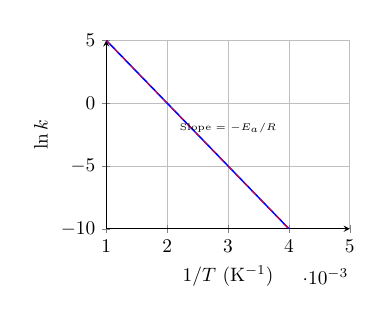
\begin{tikzpicture}[scale=0.7]
\begin{axis}[
    xlabel={$1/T$ (K$^{-1}$)},
    ylabel={$\ln k$},
    axis lines=left,
    grid=major,
    width=6cm,
    height=5cm,
    xmin=0.001, xmax=0.005,
    ymin=-10, ymax=5
]
% Correct Arrhenius plot: ln k decreases as 1/T increases (T decreases)
\addplot[blue, thick, domain=0.001:0.005, samples=50] {10 - 5000*x};
\draw[dashed, red] (axis cs:0.001,5) -- (axis cs:0.005,-15);
\node at (axis cs:0.003,-2) {\tiny Slope = $-E_a/R$};
\end{axis}
\end{tikzpicture}
\end{columns}

\end{frame}

% ===========================================================================
% Slide: Unimolecular Reactions - The Lindemann Mechanism
% ===========================================================================
\begin{frame}{Unimolecular Reactions: The Lindemann Mechanism}

\textbf{Problem:} How can A $\to$ P be explained by collision theory?

\textbf{Lindemann-Hinshelwood Mechanism (1922):}

\begin{enumerate}
\item \textbf{Activation:} A + M $\xrightarrow{k_a}$ A$^*$ + M
\item \textbf{Deactivation:} A$^*$ + M $\xrightarrow{k_a'}$ A + M
\item \textbf{Reaction:} A$^*$ $\xrightarrow{k_b}$ P
\end{enumerate}

\vspace{0.15cm}

\textbf{Key Idea:}
\begin{itemize}
\item A$^*$ = high-energy form of A
\item M = any collision partner
\item Competition: deactivation vs. reaction
\end{itemize}

\emphbox{Two limiting regimes: high pressure and low pressure}

\end{frame}

% ===========================================================================
% Slide: Lindemann Mechanism - Rate Law
% ===========================================================================
\begin{frame}{Lindemann Mechanism: Deriving the Rate Law}

\textbf{Mechanism:}
\begin{align*}
\text{A} + \text{M} &\underset{k_a'}{\overset{k_a}{\rightleftharpoons}} \text{A}^* + \text{M} \\
\text{A}^* &\xrightarrow{k_b} \text{P}
\end{align*}

\textbf{Rate of product formation:} $\frac{d[\text{P}]}{dt} = k_b[\text{A}^*]$

\textbf{Steady-state approximation for A$^*$:}
\[ \frac{d[\text{A}^*]}{dt} = k_a[\text{A}][\text{M}] - k_a'[\text{A}^*][\text{M}] - k_b[\text{A}^*] = 0 \]

\textbf{Solve for [A$^*$]:}
\[ [\text{A}^*] = \frac{k_a[\text{A}][\text{M}]}{k_a'[\text{M}] + k_b} \]

\textbf{Overall rate:}
\keyeq{\frac{d[\text{P}]}{dt} = \frac{k_a k_b [\text{M}]}{k_a'[\text{M}] + k_b} [\text{A}]}

\end{frame}

% ===========================================================================
% Slide: Lindemann - High Pressure Limit
% ===========================================================================
\begin{frame}{Lindemann Mechanism: High Pressure Limit}

\textbf{General Rate Law:}
\[ \frac{d[\text{P}]}{dt} = \frac{k_a k_b [\text{M}]}{k_a'[\text{M}] + k_b} [\text{A}] = k_{uni}[\text{A}] \]

\vspace{0.2cm}

\textbf{High Pressure Limit:} $k_a'[\text{M}] \gg k_b$ (fast deactivation)

\[ k_{uni} \approx \frac{k_a k_b}{k_a'} = K_{eq} k_b \]

\vspace{0.15cm}

\textbf{Characteristics:}
\begin{itemize}
\item First-order in [A]
\item Independent of pressure
\item Rate-determining step: A$^* \to$ P
\item Equilibrium established between A and A$^*$
\item Collisions are frequent enough to maintain equilibrium
\end{itemize}

\end{frame}

% ===========================================================================
% Slide: Lindemann - Low Pressure Limit
% ===========================================================================
\begin{frame}{Lindemann Mechanism: Low Pressure Limit}

\textbf{General Rate Law:}
\[ k_{uni} = \frac{k_a k_b [\text{M}]}{k_a'[\text{M}] + k_b} \]

\vspace{0.4cm}

\textbf{Low Pressure Limit:} $k_a'[\text{M}] \ll k_b$ (slow activation)

\[ k_{uni} \approx k_a[\text{M}] \]

\vspace{0.3cm}

\textbf{Characteristics:}
\begin{itemize}
\item Pseudo-second-order (depends on [M])
\item Proportional to pressure
\item Rate-determining step: A + M $\to$ A$^*$
\item Every A$^*$ formed reacts immediately ($k_b$ is fast)
\item Collisions are rare, activation is limiting
\end{itemize}

\vspace{0.3cm}

\emphbox{Transition from second-order to first-order as pressure increases}

\end{frame}

% ===========================================================================
% Slide: Lindemann Plot
% ===========================================================================
\begin{frame}{Lindemann Mechanism: Graphical Representation}

\textbf{Rearrange to Lindemann form:}
\[ \frac{1}{k_{uni}} = \frac{1}{k_\infty} + \frac{k_a'}{k_a k_b[\text{M}]} = \frac{1}{k_\infty} + \frac{1}{k_a[\text{M}]} \]

where $k_\infty = \frac{k_a k_b}{k_a'}$ is the high-pressure limit.

\begin{columns}[T]
\column{0.5\textwidth}
\textbf{Lindemann Plot:}
$1/k_{uni}$ vs $1/[\text{M}]$
\begin{itemize}
\item Linear relationship
\item Intercept = $1/k_\infty$
\item Slope = $1/k_a$
\end{itemize}

\column{0.5\textwidth}
\centering
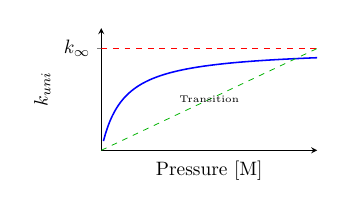
\begin{tikzpicture}[scale=0.7]
\begin{axis}[
    xlabel={Pressure [M]},
    ylabel={$k_{uni}$},
    axis lines=left,
    xmin=0, xmax=10,
    ymin=0, ymax=6,
    xtick=\empty,
    ytick={5},
    yticklabels={$k_\infty$},
    width=5.5cm,
    height=3.8cm
]
\addplot[blue, thick, domain=0.1:10, samples=100] {5*x/(x+1)};
\draw[dashed, red] (axis cs:0,5) -- (axis cs:10,5) node[right] {\tiny First-order};
\draw[dashed, green!70!black] (axis cs:0,0) -- (axis cs:10,5) node[below right] {\tiny Second-order};
\node at (axis cs:5,2.5) {\tiny Transition};
\end{axis}
\end{tikzpicture}
\end{columns}

\vspace{0.1cm}

{\small \textbf{Experimental verification:} Many unimolecular reactions show exactly this behavior!}

\end{frame}

% ===========================================================================
% Slide: RRK Theory - Part 1
% ===========================================================================
\begin{frame}{RRK Theory: Energy Distribution in Molecules (Part 1)}

\textbf{Rice-Ramsperger-Kassel (RRK) Theory:}

Refines Lindemann by considering \textit{how} energy is distributed within A$^*$.

\vspace{0.3cm}

\textbf{Key Assumptions:}
\begin{itemize}
\item Molecule has $s$ equivalent oscillators (vibrational modes)
\item Energy $E$ is distributed randomly among these modes (statistical)
\item Reaction occurs when energy $E_0$ accumulates in the reactive bond
\item Energy flows freely between modes (ergodic hypothesis)
\end{itemize}

\vspace{0.3cm}

\textbf{Key Question:} What is the probability that the reactive bond has enough energy to break?

\end{frame}

% ===========================================================================
% Slide: RRK Theory - Part 2
% ===========================================================================
\begin{frame}{RRK Theory: Energy-Dependent Rate Constant (Part 2)}

\textbf{Probability that reactive bond has energy $\ge E_0$:}
\[ P(E_0|E) = \left(1 - \frac{E_0}{E}\right)^{s-1} \quad \text{for } E \ge E_0 \]

\vspace{0.3cm}

\textbf{Energy-dependent rate constant:}
\keyeq{k_b(E) = k_b^0 \left(1 - \frac{E_0}{E}\right)^{s-1}}

\vspace{0.3cm}

\textbf{Physical Interpretation:}
\begin{itemize}
\item Higher $s$ (more oscillators): Energy more diluted, slower reaction
\item Larger molecules: Smaller $k_b(E)$ at given $E$
\item Explains why large molecules fall off more rapidly in Lindemann plots
\end{itemize}

\end{frame}

% ===========================================================================
% Slide: Summary of Collision Theory
% ===========================================================================
\begin{frame}{Summary: Collision Theory}

\textbf{Achievements:}
\begin{itemize}
\item[\checkmark] Derived rate constant from first principles (kinetic theory)
\item[\checkmark] Explained Arrhenius form: $k = A e^{-E_a/RT}$
\item[\checkmark] Calculated $A$-factors ($\sim 10^{10}-10^{11}$ dm$^3$ mol$^{-1}$ s$^{-1}$)
\item[\checkmark] Lindemann mechanism explains unimolecular reactions
\item[\checkmark] Qualitative understanding of steric effects
\end{itemize}

\vspace{0.3cm}

\textbf{Limitations:}
\begin{itemize}
\item[\xmark] Steric factor $P$ is empirical (must be measured)
\item[\xmark] Hard-sphere model too simplistic
\item[\xmark] Doesn't explain molecular details of reaction pathway
\item[\xmark] No information about transition state structure
\end{itemize}

\vspace{0.3cm}

\emphbox{Next: Transition-State Theory provides molecular-level insight}

\end{frame}

% ===========================================================================
% Slide: Practice Problems
% ===========================================================================
\begin{frame}{Practice Problems}

\textbf{Problem 1:} Calculate the collision frequency $Z_{O_2-O_2}$ for oxygen at 300 K and 1 atm. Use $\sigma = 0.40$ nm$^2$.

\vspace{0.2cm}

\textbf{Problem 2:} For the reaction H$_2$ + I$_2 \to$ 2HI, $E_a = 171$ kJ mol$^{-1}$. What fraction of collisions at 600 K have sufficient energy to react?

\vspace{0.2cm}

\textbf{Problem 3:} A reaction has $A_{exp} = 2.5 \times 10^{9}$ dm$^3$ mol$^{-1}$ s$^{-1}$ and $A_{theory} = 5.0 \times 10^{11}$ dm$^3$ mol$^{-1}$ s$^{-1}$. Calculate the steric factor $P$. What does this tell you about the reaction?

\vspace{0.2cm}

\textbf{Problem 4:} For a Lindemann mechanism with $k_\infty = 1.0 \times 10^5$ s$^{-1}$ and $k_a = 1.0 \times 10^{-10}$ dm$^3$ mol$^{-1}$ s$^{-1}$, at what pressure (in torr) does $k_{uni} = k_\infty/2$? (T = 300 K)

\vspace{0.2cm}

\textit{Answers: (1) $\sim 10^{35}$ m$^{-3}$ s$^{-1}$; (2) $e^{-171000/(8.314 \times 600)} \approx 1.7 \times 10^{-15}$; (3) $P = 0.005$, highly orientation-dependent; (4) $\sim 0.04$ torr}

\end{frame}

% ===========================================================================
% Slide: Interactive Resources for Topic 18A
% ===========================================================================
\begin{frame}{Interactive Learning: Topic 18A}

\begin{columns}[c]
\column{0.65\textwidth}
\textbf{Explore Collision Theory Interactively!}

\vspace{0.3cm}

\textbf{Interactive Jupyter Notebook Features:}
\begin{itemize}
    \item \textbf{Collision Calculator}: Adjust T, P, $\sigma$ with sliders
    \item \textbf{Animated Collisions}: Watch molecules collide!
    \item \textbf{Energy-Dependent $\sigma(\varepsilon)$}: Interactive plots
    \item \textbf{Harpoon Mechanism Explorer}: See long-range ET
    \item \textbf{RRK Model}: Explore unimolecular decay
    \item \textbf{Practice Problems}: Code-based exercises
\end{itemize}

\vspace{0.3cm}

\textbf{Notebook:} \texttt{01\_Collision\_Theory.ipynb}

\column{0.35\textwidth}
\centering
\textbf{Scan to Open:}

\vspace{0.3cm}

\includegraphics[width=0.8\textwidth]{QR_codes/01_Collision_Theory.png}

\vspace{0.3cm}

{\footnotesize Or navigate to:\\
\texttt{Reaction\_Dynamics\_Interactive/}}

\end{columns}

\end{frame}

% ============================================================================
% TOPIC 18B: DIFFUSION-CONTROLLED REACTIONS
% ============================================================================

\section{Topic 18B: Diffusion-Controlled Reactions}

% ===========================================================================
% Slide 21: Topic 18B Overview
% ===========================================================================
\begin{frame}{Topic 18B: Diffusion-Controlled Reactions}

\textbf{Moving from Gas to Liquid Phase}

\vspace{0.3cm}

\begin{columns}[T]
\column{0.5\textwidth}
\textbf{Gas Phase:}
\begin{itemize}
\item Molecules fly freely
\item Single collisions
\item Low density ($\sim 10^{25}$ m$^{-3}$)
\item Long mean free path ($\sim$ 100 nm)
\item Collision frequency $\sim 10^{10}$ s$^{-1}$
\end{itemize}

\vspace{0.2cm}
\textbf{Liquid Phase:}
\begin{itemize}
\item Molecules are crowded
\item \alert{Cage Effect} - trapped by solvent
\item High density ($\sim 10^{28}$ m$^{-3}$)
\item Short mean free path ($\sim$ 0.3 nm)
\item \alert{Diffusion} limits encounter rate
\end{itemize}

\column{0.5\textwidth}
\centering
\textbf{Solvent Cage Effect:}

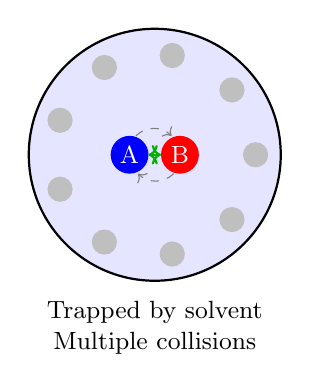
\begin{tikzpicture}[scale=0.8]
    % Cage effect diagram
    \draw[fill=blue!10, thick] (0,0) circle (2cm);

    % Solvent molecules forming cage
    \foreach \angle in {0,40,80,120,160,200,240,280,320}
        \fill[gray!50] ({1.6*cos(\angle)}, {1.6*sin(\angle)}) circle (0.2cm);

    % Reactant molecules inside cage
    \fill[blue] (-0.4,0) circle (0.3cm) node[white] {\small A};
    \fill[red] (0.4,0) circle (0.3cm) node[white] {\small B};

    % Multiple collision arrows
    \draw[<->, thick, green!70!black] (-0.1,0) -- (0.1,0);
    \draw[->, dashed, gray] (-0.3,0.3) arc (135:45:0.4);
    \draw[->, dashed, gray] (0.3,-0.3) arc (-45:-135:0.4);

    \node at (0,-2.5) {\small Trapped by solvent};
    \node at (0,-3) {\small Multiple collisions};
\end{tikzpicture}
\end{columns}

\end{frame}

% ===========================================================================
% Slide: Encounter Pairs
% ===========================================================================
\begin{frame}{The Concept of Encounter Pairs}

\begin{block}{Encounter Pair}
When two reactants A and B meet in solution, they are temporarily trapped in a solvent cage and undergo multiple collisions before separating.
\end{block}

\vspace{0.15cm}

\begin{columns}[T]
\column{0.5\textwidth}
\textbf{Key Differences from Gas Phase:}
\begin{itemize}
\item \textbf{Gas:} One collision per encounter
\item \textbf{Liquid:} $\sim 10^2 - 10^3$ collisions per encounter
\item Collision frequency within cage: $\sim 10^{13}$ s$^{-1}$
\item Cage lifetime: $\sim 10^{-11}$ s
\item Effective "single" encounter
\end{itemize}

\column{0.5\textwidth}
\centering
\textbf{Encounter Dynamics:}

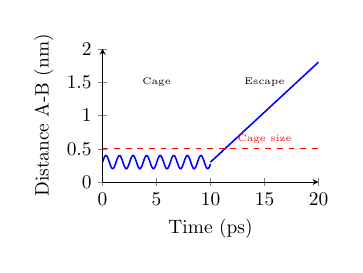
\begin{tikzpicture}[scale=0.7]
\begin{axis}[
    xlabel={Time (ps)},
    ylabel={Distance A-B (nm)},
    xmin=0, xmax=20,
    ymin=0, ymax=2,
    axis lines=left,
    width=5.5cm,
    height=4cm
]
% Oscillating distance representing cage dynamics
\addplot[blue, thick, domain=0:10, samples=100] {0.3 + 0.1*sin(deg(x*5))};
\addplot[blue, thick, domain=10:20, samples=50] {0.3 + (x-10)*0.15};
\draw[dashed, red] (axis cs:0,0.5) -- (axis cs:20,0.5);
\node[red] at (axis cs:15,0.65) {\tiny Cage size};
\node at (axis cs:5,1.5) {\tiny Cage};
\node at (axis cs:15,1.5) {\tiny Escape};
\end{axis}
\end{tikzpicture}
\end{columns}

\vspace{0.1cm}
\emphbox{For fast reactions: Rate limited by how quickly reactants find each other}

\end{frame}

% ===========================================================================
% Slide: Two Limiting Regimes
% ===========================================================================
\begin{frame}{Two Limiting Regimes}

\begin{columns}[T]
\column{0.5\textwidth}
\begin{block}{Diffusion-Controlled}
\textbf{Fast Reaction}
\begin{itemize}
\item $k_a \gg k_{-d}$ (reaction faster than separation)
\item Every encounter leads to reaction
\item Rate limited by \alert{transport} (diffusion)
\item Low activation energy ($E_a \approx E_{viscosity}$)
\item Examples: Radical recombination, H$^+$ + OH$^-$
\end{itemize}
\vspace{0.2cm}
\keyeq{k \approx k_d \sim 10^{10} \text{ M}^{-1}\text{s}^{-1}}
\end{block}

\column{0.5\textwidth}
\begin{block}{Activation-Controlled}
\textbf{Slow Reaction}
\begin{itemize}
\item $k_a \ll k_{-d}$ (separation faster than reaction)
\item Many encounters before reaction
\item Rate limited by \alert{energy barrier}
\item High activation energy
\item Behaves like gas-phase kinetics
\end{itemize}
\vspace{0.2cm}
\keyeq{k \propto e^{-E_a/RT}}
\end{block}
\end{columns}

\vspace{0.3cm}

\textbf{The Crossover:} Many reactions show intermediate behavior!

\end{frame}

% ===========================================================================
% Slide: Mechanism of Diffusion-Controlled Reactions Part 1
% ===========================================================================
\begin{frame}{Mechanism: The Two-Step Model (Part 1)}

\textbf{Reaction Scheme:}

\[ \ch{A + B <=>[ k_d ][ k_{-d} ] [AB] ->[ k_a ] P} \]

\vspace{0.3cm}

\textbf{Elementary Steps:}
\begin{enumerate}
\item \textbf{Diffusion together:} A + B $\xrightarrow{k_d}$ [AB]
\begin{itemize}
\item $k_d$: Diffusion rate constant
\item Formation of encounter pair
\item Limited by diffusion coefficient $D$
\end{itemize}

\item \textbf{Diffusion apart:} [AB] $\xrightarrow{k_{-d}}$ A + B
\begin{itemize}
\item $k_{-d}$: Separation rate constant
\item Breakup of encounter pair
\item Also diffusion-controlled
\end{itemize}

\item \textbf{Reaction:} [AB] $\xrightarrow{k_a}$ P
\begin{itemize}
\item $k_a$: Activation rate constant
\item Chemical transformation within cage
\item Depends on $E_a$
\end{itemize}
\end{enumerate}

\end{frame}

% ===========================================================================
% Slide: Mechanism Energy Diagram
% ===========================================================================
\begin{frame}{Mechanism: Energy Diagram}

\begin{columns}[T]
\column{0.5\textwidth}
\textbf{Free Energy Profile:}

\vspace{0.2cm}

\begin{itemize}
\item A + B $\to$ [AB]: Diffusion barrier (small)
\item [AB] $\to$ [AB]$^\ddagger$: Activation barrier
\item [AB]$^\ddagger$ $\to$ P: Reaction
\end{itemize}

\vspace{0.3cm}

The rate-limiting step depends on relative barrier heights!

\column{0.5\textwidth}
\centering
\textbf{Energy Diagram:}

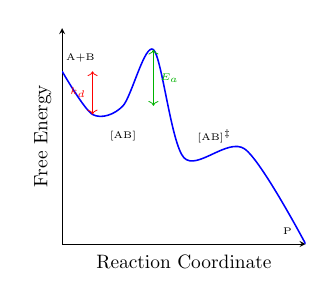
\begin{tikzpicture}[scale=0.7]
\begin{axis}[
    xlabel={Reaction Coordinate},
    ylabel={Free Energy},
    xmin=0, xmax=4,
    ymin=0, ymax=5,
    axis lines=left,
    xtick=\empty,
    ytick=\empty,
    width=6cm,
    height=5.5cm
]
% Energy profile
\addplot[blue, thick, smooth] coordinates {
    (0,4) (0.5,3) (1,3.2) (1.5,4.5) (2,2) (3,2.2) (4,0)
};
\node at (axis cs:0.3,4.3) {\tiny A+B};
\node at (axis cs:1,2.5) {\tiny [AB]};
\node at (axis cs:2.5,2.5) {\tiny [AB]$^\ddagger$};
\node at (axis cs:3.7,0.3) {\tiny P};

% Arrows
\draw[<->, red] (axis cs:0.5,3) -- (axis cs:0.5,4) node[midway, left] {\tiny $k_d$};
\draw[<->, green!70!black] (axis cs:1.5,3.2) -- (axis cs:1.5,4.5) node[midway, right] {\tiny $E_a$};
\end{axis}
\end{tikzpicture}
\end{columns}

\end{frame}

% ===========================================================================
% Slide: Steady-State Treatment Part 1
% ===========================================================================
\begin{frame}{Steady-State Treatment (Part 1)}

\textbf{Apply steady-state approximation to encounter pair [AB]:}

\[ \frac{d[\text{AB}]}{dt} = k_d[A][B] - k_{-d}[\text{AB}] - k_a[\text{AB}] = 0 \]

\vspace{0.3cm}

\textbf{Solve for [AB]:}
\[ [\text{AB}] = \frac{k_d[A][B]}{k_{-d} + k_a} \]

\vspace{0.3cm}

\textbf{Rate of product formation:}
\[ \text{Rate} = k_a[\text{AB}] = \frac{k_a k_d}{k_{-d} + k_a} [A][B] \]

\end{frame}

% ===========================================================================
% Slide: Steady-State Treatment Part 2
% ===========================================================================
\begin{frame}{Steady-State Treatment (Part 2)}

\textbf{Overall rate constant:}
\[ k_{eff} = \frac{k_a k_d}{k_{-d} + k_a} \]

\vspace{0.3cm}

\textbf{Rearrange to resistance form:}
\keyeq{\frac{1}{k_{eff}} = \frac{1}{k_d} + \frac{1}{K k_a}}

where $K = k_d/k_{-d}$ is the equilibrium constant for encounter pair formation.

\vspace{0.3cm}

\emphbox{Two resistances in series: diffusion and activation}

\vspace{0.3cm}

\textbf{Interpretation:} Like electrical resistances, the slower step dominates!

\end{frame}

% ===========================================================================
% Slide: Limiting Cases Derived
% ===========================================================================
\begin{frame}{Limiting Cases from the General Expression}

\textbf{General Result:}
\[ k_{eff} = \frac{k_a k_d}{k_{-d} + k_a} \]

\vspace{0.3cm}

\begin{columns}[T]
\column{0.5\textwidth}
\textbf{Case 1: Diffusion Control}

$k_a \gg k_{-d}$ (fast reaction)

\[ k_{eff} = \frac{k_a k_d}{k_a} = k_d \]

\begin{itemize}
\item Rate independent of $k_a$
\item Maximum possible rate
\item $k_{eff} \sim 10^{10}$ M$^{-1}$ s$^{-1}$
\item Weak temperature dependence
\item $E_a \approx E_{viscosity} \approx 10-20$ kJ/mol
\end{itemize}

\column{0.5\textwidth}
\textbf{Case 2: Activation Control}

$k_a \ll k_{-d}$ (slow reaction)

\[ k_{eff} = \frac{k_d}{k_{-d}} k_a = K k_a \]

\begin{itemize}
\item Rate proportional to $k_a$
\item Arrhenius behavior
\item Strong temperature dependence
\item $E_a$ = activation barrier
\item Same as gas-phase kinetics
\end{itemize}
\end{columns}

\vspace{0.3cm}

\textbf{Physical Interpretation:} In activation control, pairs form and break many times before reacting (equilibrium established).

\end{frame}

% ===========================================================================
% Slide: Fick's First Law
% ===========================================================================
\begin{frame}{Fick's First Law of Diffusion}

\textbf{Foundation of Diffusion Theory:}

\vspace{0.3cm}

\textbf{Fick's First Law} (steady-state):
\keyeq{J = -D \frac{\partial c}{\partial x}}

\vspace{0.3cm}

\textbf{Physical Interpretation:}
\begin{itemize}
\item $J$: Flux (mol m$^{-2}$ s$^{-1}$) - flow rate per unit area
\item $D$: Diffusion coefficient (m$^2$ s$^{-1}$)
\item $\frac{\partial c}{\partial x}$: Concentration gradient
\item Negative sign: Flow from high to low concentration
\end{itemize}

\vspace{0.3cm}

\textbf{Typical Values:} $D \sim 10^{-9}$ m$^2$ s$^{-1}$ in water (small molecules)

\end{frame}

% ===========================================================================
% Slide: Fick's Second Law
% ===========================================================================
\begin{frame}{Fick's Second Law of Diffusion}

\textbf{Fick's Second Law} (time-dependent):
\keyeq{\frac{\partial c}{\partial t} = D \frac{\partial^2 c}{\partial x^2}}

\vspace{0.3cm}

\textbf{Physical Interpretation:}
\begin{itemize}
\item Describes how concentration evolves in time
\item Parabolic partial differential equation (diffusion/heat equation)
\item In 3D: $\frac{\partial c}{\partial t} = D \nabla^2 c$
\item Solution gives $c(x,t)$ - concentration distribution
\end{itemize}

\vspace{0.3cm}

\emphbox{These laws form the mathematical foundation for Smoluchowski theory}

\end{frame}

% ===========================================================================
% Slide: Stokes-Einstein Relation Part 1
% ===========================================================================
\begin{frame}{Stokes-Einstein Relation (Part 1)}

\textbf{Connection between diffusion and molecular properties:}

\vspace{0.3cm}

For a spherical particle of radius $r$ moving through liquid of viscosity $\eta$:

\keyeq{D = \frac{k_B T}{6\pi \eta r}}

\vspace{0.3cm}

\textbf{Physical Basis:}
\begin{itemize}
\item Stokes drag force: $F = 6\pi \eta r v$
\item Einstein relation: $D = \mu k_B T$ where $\mu = 1/6\pi\eta r$
\item Connects microscopic (diffusion) to macroscopic (viscosity)
\end{itemize}

\vspace{0.3cm}

\textbf{Key Dependencies:}
\begin{itemize}
\item $D \propto T$ (faster at higher temperature)
\item $D \propto 1/\eta$ (slower in viscous media)
\item $D \propto 1/r$ (smaller molecules diffuse faster)
\end{itemize}

\end{frame}

% ===========================================================================
% Slide: Stokes-Einstein Relation Part 2
% ===========================================================================
\begin{frame}{Stokes-Einstein Relation (Part 2)}

\begin{columns}[T]
\column{0.5\textwidth}
\textbf{Typical Values at 25°C:}

\begin{table}
\small
\begin{tabular}{lcc}
\toprule
\textbf{Species} & $r$ (nm) & $D$ (10$^{-9}$ m$^2$/s) \\
\midrule
H$_2$O & 0.14 & 2.3 \\
Glycerol & 0.3 & 1.0 \\
Hemoglobin & 3.1 & 0.069 \\
\bottomrule
\end{tabular}
\end{table}

\column{0.5\textwidth}
\textbf{Viscosity of Water:}
\begin{itemize}
\item 25°C: $\eta = 0.89$ mPa$\cdot$s
\item 0°C: $\eta = 1.79$ mPa$\cdot$s
\item Strong T-dependence!
\end{itemize}

\vspace{0.3cm}

\textbf{Observation:}
\begin{itemize}
\item Larger molecules: smaller $D$
\item Size effect is dramatic (factor of 30!)
\end{itemize}
\end{columns}

\vspace{0.3cm}

\emphbox{Stokes-Einstein is remarkably accurate for molecules in solution}

\end{frame}

% ===========================================================================
% Slide: Smoluchowski Theory - Setup
% ===========================================================================
\begin{frame}{Smoluchowski Theory: Deriving $k_d$}

\textbf{Goal:} Calculate the rate constant for diffusion-controlled encounter.

\vspace{0.2cm}

\textbf{Model Assumptions:}
\begin{enumerate}
\item Molecule A is stationary at origin
\item B molecules diffuse toward A with diffusion coefficient $D = D_A + D_B$
\item Reaction occurs when B reaches distance $R^* = r_A + r_B$ (contact)
\item Steady-state concentration profile of B around A
\item B molecules are consumed at $r = R^*$ (perfect sink)
\end{enumerate}

\vspace{0.2cm}

\textbf{Boundary Conditions:}
\begin{itemize}
\item At $r = R^*$: $[B] = 0$ (instantaneous reaction)
\item As $r \to \infty$: $[B] = [B]_{bulk}$ (uniform far away)
\end{itemize}

\vspace{0.2cm}

\emphbox{Solve Fick's law in spherical coordinates with these boundary conditions}

\end{frame}

% ===========================================================================
% Slide: Smoluchowski Derivation
% ===========================================================================
\begin{frame}{Smoluchowski Derivation}

\textbf{Fick's First Law in spherical coordinates (steady-state):}
\[ J(r) = -D \frac{d[B]}{dr} \]

\textbf{Continuity equation (spherical):}
\[ \frac{1}{r^2} \frac{d}{dr}\left(r^2 J\right) = 0 \]

This gives: $r^2 J = \text{constant}$

\vspace{0.2cm}

\textbf{Solution with boundary conditions:}
\[ [B](r) = [B]_{bulk} \left(1 - \frac{R^*}{r}\right) \]

\textbf{Flux at contact surface:}
\[ J(R^*) = -D \left.\frac{d[B]}{dr}\right|_{r=R^*} = D \frac{[B]_{bulk}}{R^*} \]

\textbf{Total rate (flux × area):}
\[ \text{Rate} = 4\pi (R^*)^2 \cdot J(R^*) = 4\pi R^* D [B]_{bulk} \]

\end{frame}

% ===========================================================================
% Slide: Smoluchowski Result
% ===========================================================================
\begin{frame}{Smoluchowski Result for $k_d$}

\textbf{From flux calculation:}
\[ \text{Rate} = 4\pi R^* D [A][B] \]

\textbf{Compare with rate law:} Rate = $k_d[A][B]$

\vspace{0.2cm}

\keyeq{k_d = 4\pi R^* D N_A}

where $N_A$ converts to molar units.

\vspace{0.3cm}

\textbf{Using Stokes-Einstein:} $D = \frac{k_B T}{6\pi \eta r}$

For similar-sized molecules: $R^* \approx 2r$ and $D \approx \frac{k_B T}{6\pi \eta r}$

\keyeq{k_d \approx \frac{8RT}{3\eta}}

\vspace{0.2cm}

\textbf{Remarkable Result:}
\begin{itemize}
\item $k_d$ depends mainly on $T$ and $\eta$
\item Nearly independent of molecular size (cancellation!)
\item Universal diffusion limit for reactions in solution
\end{itemize}

\end{frame}

% ===========================================================================
% Slide: Numerical Estimate
% ===========================================================================
\begin{frame}{Numerical Estimate of Diffusion Limit}

\textbf{For water at 25°C:}

\textbf{Given:}
\begin{itemize}
\item $T = 298$ K
\item $\eta = 8.9 \times 10^{-4}$ Pa$\cdot$s
\item $R = 8.314$ J mol$^{-1}$ K$^{-1}$
\end{itemize}

\vspace{0.2cm}

\textbf{Calculation:}
\[ k_d = \frac{8RT}{3\eta} = \frac{8 \times 8.314 \times 298}{3 \times 8.9 \times 10^{-4}} \]

\[ k_d = \frac{19{,}830}{0.00267} = 7.4 \times 10^6 \text{ m}^3 \text{ mol}^{-1} \text{ s}^{-1} \]

\vspace{0.2cm}

\keyeq{k_d \approx 7 \times 10^9 \text{ dm}^3 \text{ mol}^{-1} \text{ s}^{-1} = 7 \times 10^9 \text{ M}^{-1} \text{ s}^{-1}}

\vspace{0.3cm}

\emphbox{This is the \textbf{diffusion limit}: Maximum possible rate in aqueous solution}

\textbf{Note:} If you measure $k > 10^{10}$ M$^{-1}$ s$^{-1}$, check for errors or special mechanisms (e.g., long-range forces, harpoon reactions).

\end{frame}

% ===========================================================================
% Slide: Temperature Dependence
% ===========================================================================
\begin{frame}{Temperature Dependence of Diffusion-Controlled Reactions}

\textbf{From Smoluchowski:} $k_d = \frac{8RT}{3\eta}$

\vspace{0.2cm}

\textbf{Temperature dependence comes from:}
\begin{enumerate}
\item Direct $T$ factor: $k_d \propto T$
\item Viscosity: $\eta(T)$ decreases with increasing $T$
\end{enumerate}

\vspace{0.2cm}

\textbf{Viscosity Temperature Dependence:}
\[ \eta(T) = \eta_0 e^{E_{\eta}/RT} \]

Typical values: $E_\eta \approx 10-20$ kJ/mol for liquids

\vspace{0.2cm}

\textbf{Combined effect:}
\[ k_d \propto \frac{T}{\eta(T)} \propto T e^{-E_{\eta}/RT} \]

Taking logarithm and differentiating:
\[ \frac{d \ln k_d}{d(1/T)} = -\frac{E_{\eta}}{R} + \frac{RT}{T} = -\frac{E_{\eta} - RT}{R} \]

\keyeq{E_{a,diff} \approx E_{\eta} - RT \approx E_{\eta} - 2.5 \text{ kJ/mol}}

\textbf{Typical:} $E_{a,diff} \sim 10-20$ kJ/mol (much smaller than chemical activation!)

\end{frame}

% ===========================================================================
% Slide: Comparison with Experimental Data
% ===========================================================================
\begin{frame}{Experimental Verification}

\textbf{Examples of Diffusion-Controlled Reactions:}

\vspace{0.2cm}

\begin{table}
\centering
\small
\begin{tabular}{lcc}
\toprule
\textbf{Reaction} & $k$ (M$^{-1}$ s$^{-1}$) & $E_a$ (kJ/mol) \\
\midrule
H$^+$ + OH$^-$ $\to$ H$_2$O & $1.4 \times 10^{11}$ & 13 \\
H$_3$O$^+$ + OH$^-$ & $1.3 \times 10^{11}$ & 12 \\
$\bullet$ CH$_3$ + $\bullet$ CH$_3$ & $\sim 10^{10}$ & 8 \\
Fe$^{2+}$ + Fe$^{3+}$ (exchange) & $4 \times 10^3$ & 42 \\
Sucrose hydrolysis & $5 \times 10^{-5}$ & 107 \\
\bottomrule
\end{tabular}
\end{table}

\vspace{0.3cm}

\textbf{Observations:}
\begin{itemize}
\item H$^+$/OH$^-$ faster than predicted: Proton transfer via hydrogen bonding (Grotthuss mechanism)
\item Radical recombination: Near diffusion limit
\item Fe$^{2+}$/Fe$^{3+}$: Electron transfer has barrier (Chapter 18E)
\item Sucrose: High $E_a$, clearly activation-controlled
\end{itemize}

\end{frame}

% ===========================================================================
% Slide: Viscosity Effects
% ===========================================================================
\begin{frame}{Viscosity Effects on Reaction Rates}

\textbf{Prediction:} For diffusion-controlled reactions, $k \propto 1/\eta$

\vspace{0.2cm}

\textbf{Test:} Vary solvent viscosity (add glycerol, change solvent, vary T)

\begin{columns}[T]
\column{0.5\textwidth}
\textbf{Plot:} $k$ vs $1/\eta$

\begin{itemize}
\item \textbf{Linear:} Diffusion-controlled
\item \textbf{Flat:} Activation-controlled
\item \textbf{Curved:} Intermediate or mixed control
\end{itemize}

\vspace{0.2cm}
\textbf{Kramers Theory:}

More sophisticated treatment including friction:

\[ k \propto \frac{1}{\eta} \text{ (high $\eta$)} \]
\[ k \propto \eta \text{ (low $\eta$)} \]

Transition at intermediate viscosity!

\column{0.5\textwidth}
\centering
\textbf{Rate vs Viscosity:}

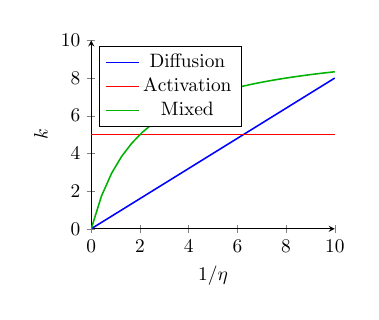
\begin{tikzpicture}[scale=0.7]
\begin{axis}[
    xlabel={$1/\eta$},
    ylabel={$k$},
    xmin=0, xmax=10,
    ymin=0, ymax=10,
    axis lines=left,
    width=6cm,
    height=5cm,
    legend pos=north west
]
\addplot[blue, thick, domain=0:10] {0.8*x};
\addlegendentry{Diffusion}

\addplot[red, thick, domain=0:10] {5};
\addlegendentry{Activation}

\addplot[green!70!black, thick, domain=0:10] {5*x/(1+0.5*x)};
\addlegendentry{Mixed}
\end{axis}
\end{tikzpicture}

\vspace{0.2cm}
\small Diffusion-controlled reactions slow down in viscous media
\end{columns}

\end{frame}

% ===========================================================================
% Slide: Material Balance Equation
% ===========================================================================
\begin{frame}{The Material Balance Equation}

\textbf{General equation for species J undergoing transport and reaction:}

\keyeq{\frac{\partial [J]}{\partial t} = D \frac{\partial^2 [J]}{\partial x^2} - v \frac{\partial [J]}{\partial x} - k_r [J]}

\vspace{0.3cm}

\textbf{Three contributions:}

\begin{enumerate}
\item \textbf{Diffusion:} $D \frac{\partial^2 [J]}{\partial x^2}$
\begin{itemize}
\item Spreading due to concentration gradients
\item Fick's second law
\item Always acts to smooth out concentration differences
\end{itemize}

\item \textbf{Convection:} $-v \frac{\partial [J]}{\partial x}$
\begin{itemize}
\item Bulk flow of fluid
\item $v$ = flow velocity
\item Important in stirred reactors, flowing systems
\end{itemize}

\item \textbf{Reaction:} $-k_r [J]$
\begin{itemize}
\item Chemical transformation
\item Acts as a sink (or source if production)
\item Local consumption
\end{itemize}
\end{enumerate}

\end{frame}

% ===========================================================================
% Slide: Diffusion-Reaction Coupling
% ===========================================================================
\begin{frame}{Coupled Diffusion and Reaction}

\textbf{Simplified 1D case (no convection):}

\[ \frac{\partial c}{\partial t} = D \frac{\partial^2 c}{\partial x^2} - kc \]

\vspace{0.2cm}

\textbf{Steady-state solution ($\partial c/\partial t = 0$):}

\[ D \frac{d^2 c}{dx^2} = kc \]

\textbf{General solution:}
\[ c(x) = A e^{-x/\lambda} + B e^{x/\lambda} \]

where the \textbf{reaction-diffusion length} is:

\keyeq{\lambda = \sqrt{\frac{D}{k}}}

\vspace{0.2cm}

\textbf{Physical Meaning:}
\begin{itemize}
\item $\lambda$: Typical distance a molecule diffuses before reacting
\item Large $\lambda$ (slow reaction): Penetrates far
\item Small $\lambda$ (fast reaction): Reacts near surface
\end{itemize}

\end{frame}

% ===========================================================================
% Slide: Example - Diffusion with Reaction
% ===========================================================================
\begin{frame}{Example: Iodine Diffusion in Starch Solution}

\textbf{Experiment:} I$_2$ vapor diffuses into aqueous starch solution where it reacts:

\[ \text{I}_2 + \text{starch} \to \text{blue complex} \]

\vspace{0.2cm}

\begin{columns}[T]
\column{0.55\textwidth}
\textbf{Observation:}
\begin{itemize}
\item Sharp blue front moves down column
\item Front position: $x_f \propto \sqrt{t}$
\item Width of colored region $\sim \lambda$
\end{itemize}

\vspace{0.2cm}
\textbf{Analysis:}

With $D = 2 \times 10^{-9}$ m$^2$ s$^{-1}$ and $k = 0.1$ s$^{-1}$:

\[ \lambda = \sqrt{\frac{D}{k}} = \sqrt{\frac{2 \times 10^{-9}}{0.1}} = 1.4 \times 10^{-4} \text{ m} = 0.14 \text{ mm} \]

Sharp front because fast reaction confines I$_2$ to thin layer.

\column{0.45\textwidth}
\centering
\textbf{Concentration Profile:}

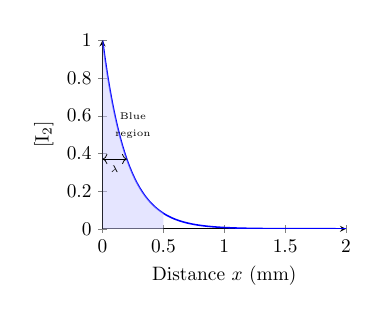
\begin{tikzpicture}[scale=0.7]
\begin{axis}[
    xlabel={Distance $x$ (mm)},
    ylabel={[I$_2$]},
    xmin=0, xmax=2,
    ymin=0, ymax=1,
    axis lines=left,
    width=6cm,
    height=5cm
]
\addplot[blue, thick, domain=0:2, samples=100] {exp(-5*x)};
\addplot[fill=blue!20, draw=none, opacity=0.5, domain=0:0.5, samples=50] {exp(-5*x)} \closedcycle;
\node at (axis cs:0.25,0.6) {\tiny Blue};
\node at (axis cs:0.25,0.5) {\tiny region};
\draw[<->] (axis cs:0,0.37) -- (axis cs:0.2,0.37) node[midway, below] {\tiny $\lambda$};
\end{axis}
\end{tikzpicture}
\end{columns}

\textbf{Application:} Pattern formation in biology (morphogen gradients), catalysis (porous catalysts)

\end{frame}

% ===========================================================================
% Slide: Damköhler Number
% ===========================================================================
\begin{frame}{The Damköhler Number}

\textbf{Dimensionless parameter comparing reaction and diffusion rates:}

\keyeq{\text{Da} = \frac{\text{reaction rate}}{\text{diffusion rate}} = \frac{kL^2}{D}}

where $L$ is characteristic length scale.

\vspace{0.3cm}

\textbf{Physical Interpretation:}

\begin{columns}[T]
\column{0.5\textwidth}
\textbf{Da $\ll$ 1:} Diffusion-limited
\begin{itemize}
\item Reaction is slow
\item Concentration uniform
\item Well-mixed approximation valid
\item Rate $\propto k$
\end{itemize}

\textbf{Da $\gg$ 1:} Mass-transfer limited
\begin{itemize}
\item Reaction is fast
\item Steep concentration gradients
\item Rate $\propto D/L$
\item Transport controls
\end{itemize}

\column{0.5\textwidth}
\centering
\textbf{Concentration Profiles:}

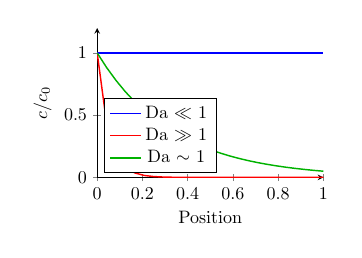
\begin{tikzpicture}[scale=0.65]
\begin{axis}[
    xlabel={Position},
    ylabel={$c/c_0$},
    xmin=0, xmax=1,
    ymin=0, ymax=1.2,
    axis lines=left,
    width=6cm,
    height=4.5cm,
    legend pos=south west
]
\addplot[blue, thick, domain=0:1] {1};
\addlegendentry{Da $\ll$ 1}

\addplot[red, thick, domain=0:1] {exp(-20*x)};
\addlegendentry{Da $\gg$ 1}

\addplot[green!70!black, thick, domain=0:1] {exp(-3*x)};
\addlegendentry{Da $\sim$ 1}
\end{axis}
\end{tikzpicture}
\end{columns}

\vspace{0.2cm}

\textbf{Applications:} Chemical reactors, catalysis, biological systems

\end{frame}

% ===========================================================================
% Slide: Worked Example 1
% ===========================================================================
\begin{frame}{Worked Example 1: Calculate $k_d$ for Specific Molecules}

\textbf{Problem:} Calculate the diffusion-controlled rate constant for the reaction between two identical molecules with $r = 0.5$ nm in water at 25°C.

\vspace{0.2cm}

\textbf{Given:}
\begin{itemize}
\item $r_A = r_B = 0.5$ nm = $5 \times 10^{-10}$ m
\item $T = 298$ K
\item $\eta_{water} = 8.9 \times 10^{-4}$ Pa$\cdot$s
\item $k_B = 1.381 \times 10^{-23}$ J K$^{-1}$
\item $N_A = 6.022 \times 10^{23}$ mol$^{-1}$
\end{itemize}

\vspace{0.2cm}

\textbf{Solution:}

\textbf{1. Contact distance:} $R^* = r_A + r_B = 1.0$ nm = $1.0 \times 10^{-9}$ m

\textbf{2. Diffusion coefficient for each molecule:}
\[ D = \frac{k_B T}{6\pi \eta r} = \frac{1.381 \times 10^{-23} \times 298}{6\pi \times 8.9 \times 10^{-4} \times 5 \times 10^{-10}} = 4.9 \times 10^{-10} \text{ m}^2\text{ s}^{-1} \]

\end{frame}

% ===========================================================================
% Slide: Worked Example 1 cont.
% ===========================================================================
\begin{frame}{Worked Example 1 (continued)}

\textbf{3. Combined diffusion coefficient:}
\[ D_{rel} = D_A + D_B = 2D = 9.8 \times 10^{-10} \text{ m}^2 \text{ s}^{-1} \]

\textbf{4. Smoluchowski rate constant:}
\[ k_d = 4\pi R^* D_{rel} N_A \]
\[ k_d = 4\pi \times 1.0 \times 10^{-9} \times 9.8 \times 10^{-10} \times 6.022 \times 10^{23} \]
\[ k_d = 7.4 \times 10^6 \text{ m}^3 \text{ mol}^{-1} \text{ s}^{-1} \]

\vspace{0.2cm}

\textbf{Convert to M$^{-1}$ s$^{-1}$:}
\[ k_d = 7.4 \times 10^9 \text{ M}^{-1} \text{ s}^{-1} \]

\vspace{0.3cm}

\emphbox{\textbf{Answer:} $k_d \approx 7 \times 10^9$ M$^{-1}$ s$^{-1}$ - close to universal diffusion limit!}

\end{frame}

% ===========================================================================
% Slide: Worked Example 2
% ===========================================================================
\begin{frame}{Worked Example 2: Determine Reaction Control Regime}

\textbf{Problem:} A reaction has $k_{obs} = 5 \times 10^8$ M$^{-1}$ s$^{-1}$ in water at 25°C. The activation energy is $E_a = 25$ kJ/mol. Is this reaction diffusion-controlled or activation-controlled?

\vspace{0.2cm}

\textbf{Solution:}

\textbf{1. Compare to diffusion limit:}
\[ k_d \approx 7 \times 10^9 \text{ M}^{-1} \text{ s}^{-1} \]
\[ \frac{k_{obs}}{k_d} = \frac{5 \times 10^8}{7 \times 10^9} \approx 0.07 = 7\% \]

The observed rate is only 7\% of diffusion limit.

\vspace{0.2cm}

\textbf{2. Check activation energy:}
\begin{itemize}
\item Diffusion-controlled: $E_a \sim 10-20$ kJ/mol
\item Observed: $E_a = 25$ kJ/mol (slightly higher)
\end{itemize}

\vspace{0.2cm}

\emphbox{\textbf{Conclusion:} Mixed control with significant activation barrier. Encounters are frequent, but not every encounter leads to reaction.}

\end{frame}

% ===========================================================================
% Slide: Summary
% ===========================================================================
\begin{frame}{Summary: Topic 18B}

\textbf{Key Concepts:}

\begin{enumerate}
\item \textbf{Cage Effect:} Multiple collisions within solvent cage
\begin{itemize}
\item Changes encounter dynamics vs gas phase
\item Effective single "encounter" event
\end{itemize}

\item \textbf{Two-Step Mechanism:} Diffusion + Activation
\begin{itemize}
\item $k_{eff}^{-1} = k_d^{-1} + (Kk_a)^{-1}$
\item Two resistances in series
\end{itemize}

\item \textbf{Smoluchowski Theory:} $k_d = 4\pi R^* D N_A \approx \frac{8RT}{3\eta}$
\begin{itemize}
\item Diffusion limit: $\sim 10^{10}$ M$^{-1}$ s$^{-1}$ in water
\item Depends on $T/\eta$, nearly size-independent
\end{itemize}

\item \textbf{Fick's Laws:} Foundation of diffusion theory
\begin{itemize}
\item First law: Flux proportional to gradient
\item Second law: Time evolution of concentration
\end{itemize}

\item \textbf{Material Balance:} Couples diffusion, convection, and reaction
\begin{itemize}
\item Reaction-diffusion length: $\lambda = \sqrt{D/k}$
\item Damköhler number: Da $= kL^2/D$
\end{itemize}
\end{enumerate}

\end{frame}

% ===========================================================================
% Slide: Practice Problems
% ===========================================================================
\begin{frame}{Practice Problems}

\textbf{Problem 1:} Calculate the diffusion coefficient of a spherical protein with radius 3.0 nm in water at 25°C ($\eta = 0.89$ mPa$\cdot$s).

\vspace{0.2cm}

\textbf{Problem 2:} For a reaction with $k_{obs} = 2 \times 10^9$ M$^{-1}$ s$^{-1}$ at 25°C, estimate what fraction of encounters lead to reaction. Assume $k_d = 7 \times 10^9$ M$^{-1}$ s$^{-1}$.

\vspace{0.2cm}

\textbf{Problem 3:} A reaction rate triples when temperature increases from 15°C to 35°C. The viscosity decreases by a factor of 1.8 over this range. Is the reaction diffusion-controlled or activation-controlled? Estimate $E_a$.

\vspace{0.2cm}

\textbf{Problem 4:} Calculate the reaction-diffusion length $\lambda$ for a first-order reaction with $k = 1.0$ s$^{-1}$ and $D = 10^{-9}$ m$^2$ s$^{-1}$.

\vspace{0.2cm}

\textit{Answers: (1) $D \approx 7.3 \times 10^{-11}$ m$^2$ s$^{-1}$; (2) $\sim$29\%; (3) Activation-controlled, $E_a \approx 35$ kJ/mol; (4) $\lambda \approx 30$ $\mu$m}

\end{frame}

% ===========================================================================
% Slide: Applications and Extensions
% ===========================================================================
\begin{frame}{Applications and Modern Extensions}

\textbf{Biological Systems:}
\begin{itemize}
\item Enzyme-substrate encounter ($k_{cat}/K_M$ often near diffusion limit)
\item Signal transduction cascades
\item Protein-protein interactions
\item Morphogen gradient formation
\end{itemize}

\vspace{0.2cm}

\textbf{Chemical Engineering:}
\begin{itemize}
\item Reactor design (stirring requirements)
\item Catalysis in porous media
\item Gas-liquid reactions
\item Fast reactions in flow systems
\end{itemize}

\vspace{0.2cm}

\textbf{Modern Developments:}
\begin{itemize}
\item Single-molecule tracking (fluorescence microscopy)
\item Microfluidics and confinement effects
\item Anomalous diffusion in crowded environments
\item Brownian dynamics simulations
\end{itemize}

\vspace{0.2cm}

\emphbox{Next: Transition-State Theory provides molecular details of the activation barrier}

\end{frame}

% ===========================================================================
% Slide: Interactive Resources for Topic 18B
% ===========================================================================
\begin{frame}{Interactive Learning: Topic 18B}

\begin{columns}[c]
\column{0.65\textwidth}
\textbf{Explore Diffusion-Controlled Reactions Interactively!}

\vspace{0.3cm}

\textbf{Interactive Jupyter Notebook Features:}
\begin{itemize}
    \item \textbf{Cage Effect Simulator}: Visualize solvent cage dynamics
    \item \textbf{Smoluchowski Calculator}: Compute diffusion-controlled rates
    \item \textbf{Encounter Pair Dynamics}: Animated trajectories
    \item \textbf{Viscosity Effects}: Interactive rate vs $\eta$ plots
    \item \textbf{Activation vs Diffusion}: Regime comparison
    \item \textbf{Real Examples}: Radical recombination, enzyme kinetics
\end{itemize}

\vspace{0.3cm}

\textbf{Notebook:} \texttt{02\_Diffusion\_Controlled.ipynb}

\column{0.35\textwidth}
\centering
\textbf{Scan to Open:}

\vspace{0.3cm}

\includegraphics[width=0.8\textwidth]{QR_codes/02_Diffusion_Controlled.png}

\vspace{0.3cm}

{\footnotesize Or navigate to:\\
\texttt{Reaction\_Dynamics\_Interactive/}}

\end{columns}

\end{frame}

% ============================================================================
% TOPIC 18C: TRANSITION-STATE THEORY
% ============================================================================

\section{Topic 18C: Transition-State Theory}

% ===========================================================================
% Slide 35: Topic 18C Overview
% ===========================================================================
\begin{frame}{Topic 18C: Overview}

\textbf{Transition-State Theory (TST) / Activated Complex Theory (ACT)}

\vspace{0.3cm}

\begin{itemize}
    \item The most sophisticated "classical" theory of reaction rates.
    \item Developed by Eyring, Evans, and Polanyi (1930s).
    \item \textbf{Key Concept:} Focus on the species at the top of the energy barrier.
\end{itemize}

\vspace{0.3cm}
\textbf{Goals:}
\begin{itemize}
    \item Calculate rates from thermodynamic properties ($\Delta G^\ddagger$, $\Delta H^\ddagger$, $\Delta S^\ddagger$).
    \item Explain kinetic salt effects.
    \item Explain kinetic isotope effects.
\end{itemize}

\end{frame}

% ===========================================================================
% Slide: The Reaction Coordinate
% ===========================================================================
\begin{frame}{The Reaction Coordinate}

\begin{columns}[T]
\column{0.5\textwidth}
\begin{itemize}
    \item \textbf{Reactants (A+B)}
    \item \textbf{Transition State ($\ddagger$)}: Point of maximum energy.
    \item \textbf{Activated Complex (C$^\ddagger$)}: The molecular species at the transition state.
    \item \textbf{Products (P)}
\end{itemize}

\column{0.5\textwidth}
\centering
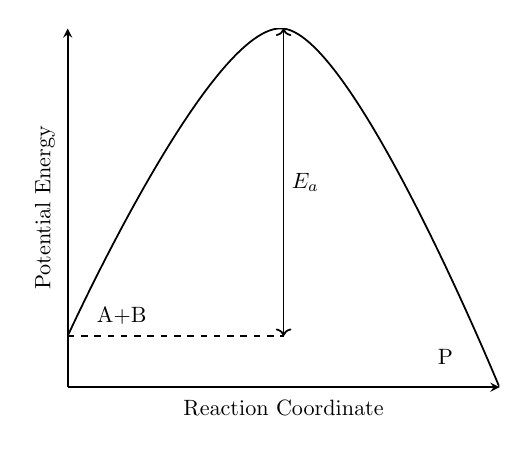
\begin{tikzpicture}[scale=0.8]
    \begin{axis}[
        xlabel={Reaction Coordinate},
        ylabel={Potential Energy},
        xtick=\empty, ytick=\empty,
        axis lines=left,
        thick
    ]
    \addplot[smooth, tension=0.6] coordinates {(0,1) (2,4) (4,0.5)};
    \node at (axis cs:0.5,1.2) {A+B};
    \node at (axis cs:2,4.3) {C$^\ddagger$};
    \node at (axis cs:3.5,0.8) {P};
    \draw[dashed] (axis cs:0,1) -- (axis cs:2,1);
    \draw[<->] (axis cs:2,1) -- (axis cs:2,4) node[midway, right] {$E_a$};
    \end{axis}
\end{tikzpicture}
\end{columns}

\end{frame}

% ===========================================================================
% Slide: Fundamental Assumptions of TST
% ===========================================================================
\begin{frame}{Fundamental Assumptions of TST}

\textbf{Three Key Assumptions:}

\begin{enumerate}
    \item \textbf{Quasi-Equilibrium:} The activated complex C$^\ddagger$ is in equilibrium with reactants.
    \[ \text{A} + \text{B} \underset{K^\ddagger}{\rightleftharpoons} \text{C}^\ddagger \]

    \item \textbf{Factorization:} The reaction coordinate motion can be separated from other degrees of freedom.

    \item \textbf{One-Way Crossing:} Once formed, C$^\ddagger$ always proceeds to products (transmission coefficient $\kappa \approx 1$).
\end{enumerate}

\vspace{0.3cm}
\textbf{Validity:} These assumptions work well when:
\begin{itemize}
    \item Barrier is high compared to $k_B T$
    \item No significant recrossing of barrier
    \item No quantum tunneling (for classical TST)
\end{itemize}

\end{frame}

% ===========================================================================
% Slide: The Big Idea
% ===========================================================================
\begin{frame}{The Big Idea}

\textbf{Fundamental Approach:}
The activated complex C$^\ddagger$ is in \alert{quasi-equilibrium} with the reactants.

\[ \text{A} + \text{B} \underset{K^\ddagger}{\rightleftharpoons} \text{C}^\ddagger \xrightarrow{k^\ddagger} \text{P} \]

\vspace{0.3cm}
The rate of reaction is:
\[ \text{Rate} = k^\ddagger [\text{C}^\ddagger] \]

\begin{itemize}
    \item $[\text{C}^\ddagger]$: Concentration of activated complex (from equilibrium).
    \item $k^\ddagger$: Frequency of crossing the barrier.
\end{itemize}

\vspace{0.3cm}
\textbf{Strategy:}
\begin{enumerate}
    \item Calculate $[\text{C}^\ddagger]$ from equilibrium thermodynamics
    \item Calculate $k^\ddagger$ from the reaction coordinate vibration frequency
    \item Combine to get the rate constant
\end{enumerate}

\end{frame}

% ===========================================================================
% Slide: Statistical Mechanics Foundation
% ===========================================================================
\begin{frame}{Statistical Mechanics Foundation}

\textbf{Partition Functions:}

For a molecular species $i$, the molecular partition function is:
\[ q_i = \sum_j g_j e^{-\varepsilon_j/k_B T} \]

The equilibrium constant relates to partition functions:
\keyeq{K^\ddagger = \frac{[\text{C}^\ddagger]}{[\text{A}][\text{B}]} = \frac{q_{\text{C}^\ddagger}}{q_{\text{A}} q_{\text{B}}} \frac{N_A}{V} e^{-E_0/RT}}

where $E_0$ is the zero-point energy difference.

\vspace{0.3cm}
\textbf{Key Insight:} The partition function includes contributions from:
\begin{itemize}
    \item Translation: $q_{\text{trans}} \propto V T^{3/2} m^{3/2}$
    \item Rotation: $q_{\text{rot}} \propto T^{3/2}$ (nonlinear)
    \item Vibration: $q_{\text{vib}} = \prod_i \frac{1}{1-e^{-h\nu_i/k_B T}}$
\end{itemize}

\end{frame}

% ===========================================================================
% Slide: Factorization of Reaction Coordinate
% ===========================================================================
\begin{frame}{Factorization of Reaction Coordinate}

\textbf{Critical Step:} Separate the reaction coordinate from $q_{\text{C}^\ddagger}$

The transition state has one "loose" vibration along the reaction coordinate with frequency $\nu^\ddagger$.

For this mode:
\[ q_{\text{RC}} = \frac{1}{1-e^{-h\nu^\ddagger/k_B T}} \approx \frac{k_B T}{h\nu^\ddagger} \quad \text{(classical limit)} \]

Therefore:
\keyeq{q_{\text{C}^\ddagger} = \left(\frac{k_B T}{h\nu^\ddagger}\right) \bar{q}_{\text{C}^\ddagger}}

where $\bar{q}_{\text{C}^\ddagger}$ is the partition function with the reaction coordinate removed.

\end{frame}

% ===========================================================================
% Slide: Rate of Decay - Vibrational Motion
% ===========================================================================
\begin{frame}{Rate of Decay}

\textbf{How fast does C$^\ddagger$ fall apart into products?}

\begin{itemize}
    \item The motion along the reaction coordinate is a "loose vibration".
    \item Frequency of this vibration = $\nu^\ddagger$.
    \item Rate constant for crossing: $k^\ddagger = \kappa \nu^\ddagger$.
    \item $\kappa$: Transmission coefficient (usually $\approx 1$).
\end{itemize}

\vspace{0.3cm}
\textbf{Physical Picture:}
\begin{itemize}
    \item At the transition state, the molecule "vibrates" along the reaction path
    \item Each vibration has a chance to proceed to products
    \item For classical barrier crossing: every forward crossing leads to products ($\kappa = 1$)
    \item For tunneling or recrossing: $\kappa \neq 1$
\end{itemize}

\end{frame}

% ===========================================================================
% Slide: Derivation of Eyring Equation - Step 1
% ===========================================================================
\begin{frame}{Derivation of Eyring Equation - Step 1}

\textbf{Concentration of activated complex:}

From equilibrium:
\[ [\text{C}^\ddagger] = K^\ddagger [\text{A}][\text{B}] \]

Substituting partition functions:
\[ [\text{C}^\ddagger] = \frac{q_{\text{C}^\ddagger}}{q_{\text{A}} q_{\text{B}}} \frac{N_A}{V} e^{-E_0/RT} [\text{A}][\text{B}] \]

Factor out reaction coordinate:
\[ [\text{C}^\ddagger] = \frac{k_B T}{h\nu^\ddagger} \frac{\bar{q}_{\text{C}^\ddagger}}{q_{\text{A}} q_{\text{B}}} \frac{N_A}{V} e^{-E_0/RT} [\text{A}][\text{B}] \]

\end{frame}

% ===========================================================================
% Slide: Derivation of Eyring Equation - Step 2
% ===========================================================================
\begin{frame}{Derivation of Eyring Equation - Step 2}

\textbf{Rate of reaction:}

\[ \text{Rate} = \kappa \nu^\ddagger [\text{C}^\ddagger] \]

Substitute expression for $[\text{C}^\ddagger]$:
\[ \text{Rate} = \kappa \nu^\ddagger \times \frac{k_B T}{h\nu^\ddagger} \frac{\bar{q}_{\text{C}^\ddagger}}{q_{\text{A}} q_{\text{B}}} \frac{N_A}{V} e^{-E_0/RT} [\text{A}][\text{B}] \]

\alert{The frequency $\nu^\ddagger$ cancels!}

\[ \text{Rate} = \kappa \frac{k_B T}{h} \frac{\bar{q}_{\text{C}^\ddagger}}{q_{\text{A}} q_{\text{B}}} \frac{N_A}{V} e^{-E_0/RT} [\text{A}][\text{B}] \]

\end{frame}

% ===========================================================================
% Slide: The Eyring Equation - Final Form
% ===========================================================================
\begin{frame}{The Eyring Equation - Final Form}

\textbf{Rate constant:}

\keyeq{k_r = \kappa \frac{k_B T}{h} \bar{K}^\ddagger}

Or in thermodynamic terms:
\keyeq{k_r = \kappa \frac{k_B T}{h} e^{-\Delta^\ddagger G^\circ / RT}}

where $\Delta^\ddagger G^\circ$ is the standard Gibbs energy of activation.

\vspace{0.3cm}
\textbf{Key Features:}
\begin{itemize}
    \item Universal pre-factor: $\frac{k_B T}{h} \approx 6.2 \times 10^{12}$ s$^{-1}$ at 298 K
    \item Temperature dependence: $T e^{-\Delta^\ddagger H^\circ / RT}$ (not just exponential!)
    \item Connection to thermodynamics through $\Delta^\ddagger G^\circ$
\end{itemize}

\end{frame}

% ===========================================================================
% Slide: Eyring Equation - Physical Interpretation
% ===========================================================================
\begin{frame}{Eyring Equation - Interpretation}

\[ k_r = \frac{k_B T}{h} e^{-\Delta^\ddagger G^\circ / RT} \]

\begin{itemize}
    \item $\frac{k_B T}{h}$: \textbf{Universal Frequency Factor}.
    \begin{itemize}
        \item At 300 K, $\approx 6 \times 10^{12}$ s$^{-1}$.
        \item Sets the fundamental timescale of chemical reactions.
        \item Origin: Typical vibrational frequency at TS.
    \end{itemize}
    \item $\Delta^\ddagger G^\circ$: \textbf{Gibbs Energy of Activation}.
    \begin{itemize}
        \item Determines the barrier height.
        \item Includes both enthalpy and entropy contributions.
        \item Can be measured experimentally.
    \end{itemize}
\end{itemize}

\vspace{0.3cm}
\textbf{Maximum Rate:} If $\Delta^\ddagger G^\circ = 0$, then $k_r \approx 6 \times 10^{12}$ s$^{-1}$ - the \alert{diffusion-limited rate}.

\end{frame}

% ===========================================================================
% Slide: Thermodynamic Formulation
% ===========================================================================
\begin{frame}{Thermodynamic Formulation}

Expand $\Delta^\ddagger G^\circ = \Delta^\ddagger H^\circ - T\Delta^\ddagger S^\circ$:

\keyeq{k_r = \frac{k_B T}{h} e^{\Delta^\ddagger S^\circ / R} e^{-\Delta^\ddagger H^\circ / RT}}

\textbf{Comparison with Arrhenius ($k = A e^{-E_a/RT}$):}
\begin{itemize}
    \item \textbf{Enthalpy ($\Delta^\ddagger H^\circ$)} $\leftrightarrow$ Activation Energy ($E_a$).
    \item \textbf{Entropy ($\Delta^\ddagger S^\circ$)} $\leftrightarrow$ Pre-exponential Factor ($A$).
\end{itemize}

\vspace{0.3cm}
\textbf{Key Advantage:} TST separates:
\begin{itemize}
    \item Energetic barrier ($\Delta^\ddagger H^\circ$)
    \item Structural/entropic effects ($\Delta^\ddagger S^\circ$)
\end{itemize}

\end{frame}

% ===========================================================================
% Slide: Relating Parameters
% ===========================================================================
\begin{frame}{Relating TST to Arrhenius Parameters}

\textbf{Enthalpy vs. Activation Energy:}

Starting from definitions:
\[ E_a = RT^2 \frac{d \ln k}{dT} \]

For Eyring equation $k = \frac{k_B T}{h} e^{-\Delta^\ddagger G^\circ / RT}$:

\begin{itemize}
    \item \textbf{Solution:} $E_a = \Delta^\ddagger H^\circ + RT$
    \item \textbf{Gas Phase (bimolecular):} $E_a = \Delta^\ddagger H^\circ + 2RT$
    \item \textbf{Gas Phase (unimolecular):} $E_a = \Delta^\ddagger H^\circ + RT$
\end{itemize}

\vspace{0.3cm}
\textbf{Entropy vs. A-Factor:}
\[ A = \frac{e k_B T}{h} e^{\Delta^\ddagger S^\circ / R} \]

where $e = 2.718$ (Euler's number).

\end{frame}

% ===========================================================================
% Slide: Eyring Plot
% ===========================================================================
\begin{frame}{Eyring Plot}

\textbf{Linearization for experimental analysis:}

Take logarithm of $k = \frac{k_B T}{h} e^{\Delta^\ddagger S^\circ / R} e^{-\Delta^\ddagger H^\circ / RT}$:

\keyeq{\ln\left(\frac{k}{T}\right) = \ln\left(\frac{k_B}{h}\right) + \frac{\Delta^\ddagger S^\circ}{R} - \frac{\Delta^\ddagger H^\circ}{RT}}

\textbf{Plot:} $\ln(k/T)$ vs. $1/T$ gives straight line
\begin{itemize}
    \item \textbf{Slope:} $-\Delta^\ddagger H^\circ / R$
    \item \textbf{Intercept:} $\ln(k_B/h) + \Delta^\ddagger S^\circ/R$
\end{itemize}

\vspace{0.3cm}
\textbf{Advantage over Arrhenius:} Direct determination of $\Delta^\ddagger H^\circ$ and $\Delta^\ddagger S^\circ$.

\end{frame}

% ===========================================================================
% Slide: Activation Entropy Part 1
% ===========================================================================
\begin{frame}{Activation Entropy ($\Delta^\ddagger S^\circ$) - Part 1}

\textbf{Physical Meaning:}

\[ \Delta^\ddagger S^\circ = S^\circ_{\text{C}^\ddagger} - S^\circ_{\text{A}} - S^\circ_{\text{B}} \]

\vspace{0.3cm}

\textbf{Negative $\Delta^\ddagger S^\circ$ (Associative):}

Transition state is \textbf{more ordered} than reactants.

\begin{itemize}
    \item Example: Dimerization ($A + A \to A_2^\ddagger$)
    \item Two molecules coming together lose translational freedom
    \item Typically: $\Delta^\ddagger S^\circ \approx -100$ to $-150$ J/(mol·K)
\end{itemize}

\end{frame}

% ===========================================================================
% Slide: Activation Entropy Part 2
% ===========================================================================
\begin{frame}{Activation Entropy ($\Delta^\ddagger S^\circ$) - Part 2}

\textbf{Positive $\Delta^\ddagger S^\circ$ (Dissociative):}

Transition state is \textbf{more disordered} than reactants.

\begin{itemize}
    \item Example: Bond breaking in unimolecular decomposition
    \item Increased vibrational freedom
    \item Typically: $\Delta^\ddagger S^\circ > 0$
\end{itemize}

\vspace{0.3cm}

\textbf{Near-Zero $\Delta^\ddagger S^\circ$:}
\begin{itemize}
    \item Similar structure to reactants
    \item Minor reorganization at transition state
\end{itemize}

\vspace{0.3cm}

\emphbox{The sign of $\Delta^\ddagger S^\circ$ reveals the geometry of the transition state}

\end{frame}

% ===========================================================================
% Slide: Free Energy Diagrams
% ===========================================================================
\begin{frame}{Free Energy Diagrams}

\textbf{Effect of $\Delta^\ddagger S^\circ$ on reaction profile:}

\begin{center}
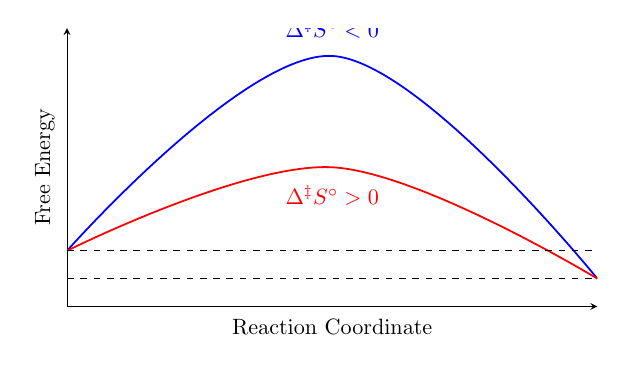
\begin{tikzpicture}[scale=0.8]
    \begin{axis}[
        xlabel={Reaction Coordinate},
        ylabel={Free Energy},
        xtick=\empty,
        ytick=\empty,
        axis lines=left,
        width=10cm,
        height=6cm,
        ymin=0, ymax=5
    ]
    % Negative entropy (higher barrier)
    \addplot[blue, thick, smooth, tension=0.6] coordinates {(0,1) (2,4.5) (4,0.5)};
    \node[blue] at (axis cs:2,5) {$\Delta^\ddagger S^\circ < 0$};

    % Positive entropy (lower barrier)
    \addplot[red, thick, smooth, tension=0.6] coordinates {(0,1) (2,2.5) (4,0.5)};
    \node[red] at (axis cs:2,2) {$\Delta^\ddagger S^\circ > 0$};

    \draw[dashed] (axis cs:0,1) -- (axis cs:4,1) node[right] {Reactants};
    \draw[dashed] (axis cs:0,0.5) -- (axis cs:4,0.5) node[right] {Products};
    \end{axis}
\end{tikzpicture}
\end{center}

At higher $T$: Negative $\Delta^\ddagger S^\circ$ becomes more unfavorable ($-T\Delta^\ddagger S^\circ$ increases).

\end{frame}

% ===========================================================================
% Slide: Hammond Postulate
% ===========================================================================
\begin{frame}{Hammond Postulate}

\textbf{Relating TS structure to thermodynamics:}

\vspace{0.3cm}
\emphbox{
\textbf{Hammond Postulate:} The structure of the transition state resembles the structure of the nearest stable species (reactant, product, or intermediate).
}

\vspace{0.3cm}
\textbf{Implications:}

\begin{columns}[T]
\column{0.5\textwidth}
\textbf{Endergonic Reaction:}
\begin{itemize}
    \item TS resembles products
    \item "Late" transition state
    \item Product-like structure
\end{itemize}

\column{0.5\textwidth}
\textbf{Exergonic Reaction:}
\begin{itemize}
    \item TS resembles reactants
    \item "Early" transition state
    \item Reactant-like structure
\end{itemize}
\end{columns}

\vspace{0.3cm}
\textbf{Application:} Helps predict effects of substituents on reaction rates.

\end{frame}

% ===========================================================================
% Slide: The Kinetic Salt Effect
% ===========================================================================
\begin{frame}{The Kinetic Salt Effect}

\textbf{For reactions between ions in solution:} $A^{z_A} + B^{z_B} \to C^\ddagger \to P$

\textbf{Debye-Hückel Theory predicts:}
\keyeq{\log(k_r) = \log(k_r^\circ) + 2A z_A z_B \sqrt{I}}

\begin{itemize}
    \item $I$: Ionic strength of solution = $\frac{1}{2}\sum_i c_i z_i^2$.
    \item $z_A, z_B$: Charges of reactants.
    \item $A$: Constant = 0.509 M$^{-1/2}$ for water at 25°C.
    \item $k_r^\circ$: Rate constant at zero ionic strength.
\end{itemize}

\vspace{0.3cm}
\textbf{Physical Origin:}
\begin{itemize}
    \item Ionic atmosphere screens charge interactions
    \item Affects activation energy for charged reactants
    \item Charge on TS: $z_\ddagger = z_A + z_B$
\end{itemize}

\end{frame}

% ===========================================================================
% Slide: Kinetic Salt Effect - Predictions Part 1
% ===========================================================================
\begin{frame}{Kinetic Salt Effect - Predictions (Part 1)}

\textbf{Effect of Ionic Strength on Rate:}

\vspace{0.3cm}

\textbf{Like charges ($z_A z_B > 0$):} Rate \alert{increases} with ionic strength.
\begin{itemize}
    \item Example: S$_2$O$_8^{2-}$ + I$^-$
    \item $z_A z_B = (-2)(-1) = +2 > 0$: rate increases
    \item Ionic atmosphere reduces repulsion
\end{itemize}

\vspace{0.3cm}

\textbf{Opposite charges ($z_A z_B < 0$):} Rate \alert{decreases} with ionic strength.
\begin{itemize}
    \item Example: [Co(NH$_3$)$_5$Br]$^{2+}$ + OH$^-$
    \item $z_A z_B = (+2)(-1) = -2 < 0$: rate decreases
    \item Ionic atmosphere screens attraction
\end{itemize}

\end{frame}

% ===========================================================================
% Slide: Kinetic Salt Effect - Predictions Part 2
% ===========================================================================
\begin{frame}{Kinetic Salt Effect - Predictions (Part 2)}

\begin{columns}[T]
\column{0.5\textwidth}
\textbf{Summary:}
\begin{itemize}
    \item $z_A z_B > 0$: rate increases with $I$
    \item $z_A z_B < 0$: rate decreases with $I$
    \item $z_A z_B = 0$: no primary salt effect
\end{itemize}

\column{0.5\textwidth}
\centering
\includegraphics[width=\textwidth]{Reaction_Dynamics_Interactive/images/kinetic_salt_effect.png}

\vspace{0.1cm}
\tiny \textit{Interactive calculator: See notebook at end}
\end{columns}

\vspace{0.3cm}

\emphbox{Slope of plot gives information about charges in the transition state}

\end{frame}

% ===========================================================================
% Slide: Kinetic Isotope Effects Part 1
% ===========================================================================
\begin{frame}{Kinetic Isotope Effects (KIE) - Part 1}

\textbf{What happens if we replace H with D (or $^{12}$C with $^{13}$C)?}

\vspace{0.3cm}

\textbf{Origin:} Zero-point energy (ZPE) difference.

\[ \text{ZPE} = \frac{1}{2}h\nu = \frac{1}{2}h\frac{1}{2\pi}\sqrt{\frac{k}{\mu}} \]

\vspace{0.3cm}

\textbf{Physical Effect:}
\begin{itemize}
    \item Heavier isotope has lower ZPE (smaller $\nu$)
    \item C-D bond is stronger than C-H bond by $\sim 5$ kJ/mol
    \item Requires more energy to break
    \item Reaction becomes slower
\end{itemize}

\vspace{0.3cm}

\keyeq{\frac{k_H}{k_D} \approx 7 \text{ (at 25}^\circ\text{C)}}

\end{frame}

% ===========================================================================
% Slide: Kinetic Isotope Effects Part 2
% ===========================================================================
\begin{frame}{Kinetic Isotope Effects (KIE) - Part 2}

\textbf{Types of KIE:}

\vspace{0.3cm}

\textbf{Primary KIE:} Bond to H/D breaks in rate-determining step
\begin{itemize}
    \item $k_H/k_D = 2$-$10$ (typical range)
    \item Large effect indicates bond breaking at TS
    \item Example: C-H bond cleavage in radical abstraction
\end{itemize}

\vspace{0.3cm}

\textbf{Secondary KIE:} Bond to H/D does not break
\begin{itemize}
    \item $k_H/k_D = 1.1$-$1.5$ (small effect)
    \item Due to hybridization changes at TS
    \item Example: Adjacent to reaction center
\end{itemize}

\vspace{0.3cm}

\emphbox{KIE is a powerful tool for identifying mechanisms and rate-determining steps}

\end{frame}

% ===========================================================================
% Slide: Zero-Point Energy Diagram
% ===========================================================================
\begin{frame}{Zero-Point Energy and KIE}

\begin{center}
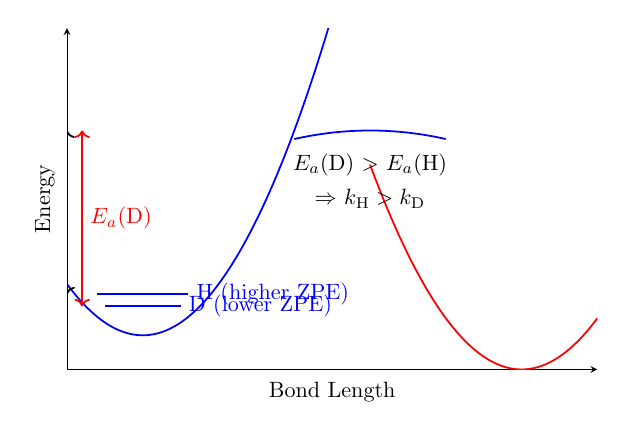
\begin{tikzpicture}[scale=0.8]
    \begin{axis}[
        xlabel={Bond Length},
        ylabel={Energy},
        xtick=\empty,
        ytick=\empty,
        axis lines=left,
        width=10cm,
        height=7cm,
        ymin=0, ymax=5
    ]
    % Reactant potential (same curvature = same force constant)
    \addplot[blue, thick, domain=0.5:2.5, samples=100] {3*(x-1)^2 + 0.5};
    % Barrier region
    \addplot[blue, thick, domain=2:3, samples=50] {3.5 - 0.5*(x-2.5)^2};
    % Product potential (same curvature as reactant)
    \addplot[red, thick, domain=2.5:4, samples=100] {3*(x-3.5)^2};

    % ZPE levels: ν ∝ √(k/m), so ZPE_D/ZPE_H = √(m_H/m_D) = 1/√2
    % Place H ZPE at 0.6 above minimum (0.5), so ZPE_H level at 1.1
    % D ZPE = 0.6/√2 = 0.424 above minimum, so level at 0.924
    \draw[blue, thick] (axis cs:0.7,1.1) -- (axis cs:1.3,1.1) node[right] {H (higher ZPE)};
    \draw[blue, thick] (axis cs:0.75,0.924) -- (axis cs:1.25,0.924) node[right] {D (lower ZPE)};

    % Activation energies (from ZPE levels to barrier top at ~3.5)
    \draw[<->, thick] (axis cs:0.5,1.1) -- (axis cs:0.5,3.5) node[midway, left] {$E_a$(H)};
    \draw[<->, thick, red] (axis cs:0.6,0.924) -- (axis cs:0.6,3.5) node[midway, right] {$E_a$(D)};

    \node at (axis cs:2.5,3) {$E_a$(D) $>$ $E_a$(H)};
    \node at (axis cs:2.5,2.5) {$\Rightarrow$ $k_{\text{H}} > k_{\text{D}}$};
    \end{axis}
\end{tikzpicture}
\end{center}

Difference in $E_a$: $\Delta E_a \approx \frac{1}{2}h(\nu_{\text{H}} - \nu_{\text{D}}) \approx 5$ kJ/mol

\end{frame}

% ===========================================================================
% Slide: Quantum Tunneling Part 1
% ===========================================================================
\begin{frame}{Quantum Tunneling (Part 1)}

\textbf{Classical TST assumes:} Over-the-barrier crossing.

\textbf{Quantum Reality:} Particles can pass \textit{through} the barrier!

\vspace{0.3cm}

\textbf{When is tunneling important?}
\begin{itemize}
    \item Significant for light particles (H$^+$, e$^-$)
    \item More important at low temperatures
    \item Pronounced for narrow, high barriers
\end{itemize}

\vspace{0.3cm}

\textbf{Experimental Evidence:}
\begin{itemize}
    \item $k_H/k_D \gg 7$ (e.g., 10-100, much larger than classical KIE)
    \item Curved Arrhenius plots (concave upward)
    \item Unusual temperature dependence (rate less sensitive to T)
\end{itemize}

\end{frame}

% ===========================================================================
% Slide: Quantum Tunneling Part 2
% ===========================================================================
\begin{frame}{Quantum Tunneling (Part 2)}

\begin{columns}[T]
\column{0.5\textwidth}
\textbf{Two Pathways:}

\vspace{0.2cm}

\textcolor{blue}{\textbf{Over:}} Classical barrier crossing

\textcolor{red}{\textbf{Through:}} Quantum tunneling

\vspace{0.3cm}

Tunneling bypasses the activation barrier!

\column{0.5\textwidth}
\centering
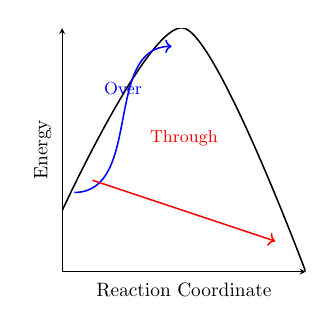
\begin{tikzpicture}[scale=0.7]
    \begin{axis}[
        xlabel={Reaction Coordinate},
        ylabel={Energy},
        xtick=\empty, ytick=\empty,
        axis lines=left,
        height=6cm,
        width=6cm
    ]
    \addplot[smooth, thick] coordinates {(0,0) (2,3) (4,-1)};
    \draw[blue, thick, ->] (0.2,0.3) to[out=0, in=180] (1.8,2.7);
    \node[blue] at (1,2) {\small Over};
    \draw[red, thick, ->] (0.5,0.5) -- (3.5,-0.5);
    \node[red] at (2,1.2) {\small Through};
    \end{axis}
\end{tikzpicture}
\end{columns}

\vspace{0.3cm}

\textbf{Bell's Correction:}
\[ \kappa = \frac{Q_{\text{tunnel}}}{Q_{\text{classical}}} = \frac{u/2}{\sin(u/2)}, \quad u = \frac{h\nu_{\text{barrier}}}{k_B T} \]

\end{frame}

% ===========================================================================
% Slide: Linear Free Energy Relationships (LFER)
% ===========================================================================
\begin{frame}{Linear Free Energy Relationships}

\textbf{Brønsted Catalysis Law:}

For acid-catalyzed reactions:
\keyeq{\log k = \log G + \alpha \log K_a}

where $K_a$ is the acidity constant.

\begin{itemize}
    \item $\alpha$: Brønsted coefficient ($0 \leq \alpha \leq 1$)
    \item Measures how much charge is transferred in TS
    \item $\alpha \approx 0$: TS resembles reactants (early TS)
    \item $\alpha \approx 1$: TS resembles products (late TS)
\end{itemize}

\vspace{0.3cm}
\textbf{Related Relationships:}
\begin{itemize}
    \item \textbf{Hammett equation:} For substituted benzene derivatives
    \item \textbf{Marcus relationship:} For electron transfer
    \item \textbf{Polanyi relationship:} $E_a = E_0 + \alpha \Delta H_{\text{rxn}}$
\end{itemize}

\end{frame}

% ===========================================================================
% Slide: Worked Example 1
% ===========================================================================
\begin{frame}{Worked Example 1: Calculating Rate Constant}

\textbf{Problem:} A reaction has $\Delta^\ddagger H^\circ = 85$ kJ/mol and $\Delta^\ddagger S^\circ = -45$ J/(mol·K). Calculate the rate constant at 298 K.

\vspace{0.3cm}
\textbf{Solution:}

Step 1: Calculate $\Delta^\ddagger G^\circ$
\[ \Delta^\ddagger G^\circ = \Delta^\ddagger H^\circ - T\Delta^\ddagger S^\circ \]
\[ = 85000 - 298 \times (-45) = 85000 + 13410 = 98410 \text{ J/mol} \]

Step 2: Apply Eyring equation
\[ k = \frac{k_B T}{h} e^{-\Delta^\ddagger G^\circ / RT} \]
\[ = \frac{1.381 \times 10^{-23} \times 298}{6.626 \times 10^{-34}} \times e^{-98410/(8.314 \times 298)} \]
\[ = 6.21 \times 10^{12} \times e^{-39.7} = 6.21 \times 10^{12} \times 7.84 \times 10^{-18} \]
\keyeq{k = 4.87 \times 10^{-5} \text{ s}^{-1}}

\end{frame}

% ===========================================================================
% Slide: Worked Example 2
% ===========================================================================
\begin{frame}{Worked Example 2: Activation Parameters from Data}

\textbf{Problem:} Rate constants measured at two temperatures:
\begin{itemize}
    \item $k(300 \text{ K}) = 1.5 \times 10^{-3}$ s$^{-1}$
    \item $k(320 \text{ K}) = 8.2 \times 10^{-3}$ s$^{-1}$
\end{itemize}
Calculate $\Delta^\ddagger H^\circ$ and $\Delta^\ddagger S^\circ$ (assume $\kappa = 1$).

\vspace{0.3cm}
\textbf{Solution:}

From Eyring plot: $\ln(k/T) = \ln(k_B/h) + \Delta^\ddagger S^\circ/R - \Delta^\ddagger H^\circ/(RT)$

Calculate slope:
\[ \text{slope} = \frac{\ln(k_2/T_2) - \ln(k_1/T_1)}{1/T_2 - 1/T_1} \]
\[ = \frac{\ln(8.2 \times 10^{-3}/320) - \ln(1.5 \times 10^{-3}/300)}{1/320 - 1/300} \]
\[ = \frac{-10.05 - (-10.72)}{-2.08 \times 10^{-4}} = \frac{0.67}{-2.08 \times 10^{-4}} = -3221 \text{ K} \]

Therefore: $\Delta^\ddagger H^\circ = -R \times \text{slope} = 8.314 \times 3221 = 26.8$ kJ/mol

\end{frame}

% ===========================================================================
% Slide: Worked Example 3
% ===========================================================================
\begin{frame}{Worked Example 3: Salt Effect}

\textbf{Problem:} For the reaction:
\[ \text{[Co(NH}_3\text{)}_5\text{Br]}^{2+} + \text{OH}^- \to \text{products} \]

The rate constant at zero ionic strength is $k_0 = 1.2 \times 10^{-4}$ M$^{-1}$s$^{-1}$. Predict the rate constant at $I = 0.05$ M.

\vspace{0.3cm}
\textbf{Solution:}

Charges: $z_A = +2$, $z_B = -1$, so $z_A z_B = -2$

Apply salt effect equation:
\[ \log(k) = \log(k_0) + 2A z_A z_B \sqrt{I} \]
\[ = \log(1.2 \times 10^{-4}) + 2(0.509)(-2)\sqrt{0.05} \]
\[ = -3.92 + 2(0.509)(-2)(0.224) = -3.92 - 0.456 = -4.38 \]

\keyeq{k = 10^{-4.38} = 4.2 \times 10^{-5} \text{ M}^{-1}\text{s}^{-1}}

The rate decreases by a factor of $\sim 3$ due to screening of attraction.

\end{frame}

% ===========================================================================
% Slide: Practice Problem 1
% ===========================================================================
\begin{frame}{Practice Problem 1}
\vspace{-0.2cm}
\textbf{Problem:} At 298 K: $\Delta^\ddagger H^\circ = 60$ kJ/mol, $\Delta^\ddagger S^\circ = -80$ J/(mol·K)

\vspace{0.15cm}
\begin{enumerate}[a),topsep=0pt,itemsep=1pt]
    \item Calculate $\Delta^\ddagger G^\circ$ at 298 K.
    \item Calculate the rate constant ($\kappa = 1$).
    \item Is TS more or less ordered?
    \item How does $k$ change at 350 K?
\end{enumerate}

\vspace{0.2cm}
\textbf{Answers:}
\begin{itemize}[topsep=0pt,itemsep=1pt]
    \item[(a)] $\Delta^\ddagger G^\circ = 83.8$ kJ/mol
    \item[(b)] $k = 9.8 \times 10^{-3}$ s$^{-1}$
    \item[(c)] More ordered ($\Delta^\ddagger S^\circ < 0$)
    \item[(d)] $k(350\text{ K}) = 0.51$ s$^{-1}$ (50$\times$ faster)
\end{itemize}

\end{frame}

% ===========================================================================
% Slide: Practice Problem 2
% ===========================================================================
\begin{frame}{Practice Problem 2}

\textbf{Problem:} The rate constant for H-abstraction by a radical is $k_{\text{H}} = 5.0 \times 10^6$ M$^{-1}$s$^{-1}$ at 298 K. The same reaction with deuterium has $k_{\text{D}} = 8.3 \times 10^5$ M$^{-1}$s$^{-1}$.

\begin{enumerate}[a)]
    \item Calculate the kinetic isotope effect $k_{\text{H}}/k_{\text{D}}$.
    \item Is this a primary or secondary KIE?
    \item What does this tell you about the mechanism?
    \item Estimate the difference in activation energies.
\end{enumerate}

\vspace{0.5cm}
\textbf{Answers:}
\begin{itemize}
    \item[(a)] KIE $= 6.0$
    \item[(b)] Primary KIE
    \item[(c)] C-H bond breaking occurs in rate-determining step
    \item[(d)] $\Delta E_a \approx 4.4$ kJ/mol (from $\ln(6.0) = \Delta E_a/(RT)$)
\end{itemize}

\end{frame}

% ===========================================================================
% Slide: Practice Problem 3
% ===========================================================================
\begin{frame}{Practice Problem 3}
\vspace{-0.2cm}
\textbf{Problem:} For an ionic reaction:

\begin{center}
\small
\begin{tabular}{cc}
$\sqrt{I}$ (M$^{1/2}$) & $k$ (M$^{-1}$s$^{-1}$) \\
\hline
0 & $2.0 \times 10^{-3}$ \\
0.1 & $3.2 \times 10^{-3}$ \\
0.2 & $5.1 \times 10^{-3}$ \\
\end{tabular}
\end{center}

\vspace{0.1cm}
\begin{enumerate}[a),topsep=0pt,itemsep=1pt]
    \item Plot $\log k$ vs $\sqrt{I}$ and find slope.
    \item Determine $z_A z_B$.
    \item Like or opposite charge?
\end{enumerate}

\vspace{0.15cm}
\textbf{Answers:}
\begin{itemize}[topsep=0pt,itemsep=1pt]
    \item[(a)] Slope $\approx 2.0$
    \item[(b)] From slope $= 2A z_A z_B$: $z_A z_B = +2$
    \item[(c)] Like charges
\end{itemize}

\end{frame}

% ===========================================================================
% Slide: Practice Problem 4
% ===========================================================================
\begin{frame}{Practice Problem 4}

\textbf{Problem:} An Eyring plot gives:
\begin{itemize}
    \item Slope $= -8500$ K
    \item Intercept $= 25.5$
\end{itemize}

Calculate $\Delta^\ddagger H^\circ$ and $\Delta^\ddagger S^\circ$.

\vspace{0.5cm}
\textbf{Solution:}

From slope:
\[ \Delta^\ddagger H^\circ = -R \times \text{slope} = 8.314 \times 8500 = 70.7 \text{ kJ/mol} \]

From intercept:
\[ \text{intercept} = \ln(k_B/h) + \Delta^\ddagger S^\circ/R \]
\[ 25.5 = 23.76 + \Delta^\ddagger S^\circ/8.314 \]
\[ \Delta^\ddagger S^\circ = (25.5 - 23.76) \times 8.314 = 14.5 \text{ J/(mol·K)} \]

\textbf{Answer:} $\Delta^\ddagger H^\circ = 70.7$ kJ/mol, $\Delta^\ddagger S^\circ = +14.5$ J/(mol·K)

Positive entropy suggests a dissociative transition state.

\end{frame}

% ===========================================================================
% Slide: Summary Topic 18C
% ===========================================================================
\begin{frame}{Summary: Topic 18C}

\begin{enumerate}
    \item \textbf{Eyring Equation:} Links rates to thermodynamics through $\Delta^\ddagger G^\circ$.
    \[ k = \frac{k_B T}{h} e^{-\Delta^\ddagger G^\circ / RT} \]

    \item \textbf{Activation Parameters:}
        \begin{itemize}
            \item $\Delta^\ddagger H^\circ \approx E_a - RT$ (solution)
            \item $\Delta^\ddagger S^\circ$ reflects structure of transition state
        \end{itemize}

    \item \textbf{Salt Effects:} Ionic strength affects rates between ions.
    \[ \log(k) = \log(k_0) + 2A z_A z_B \sqrt{I} \]

    \item \textbf{Isotope Effects:} Probe bond breaking and tunneling.
    \item \textbf{LFER:} Connect structure to reactivity (Brønsted, Hammett).
\end{enumerate}

\end{frame}

% ===========================================================================
% Slide: Interactive Resources for Topic 18C
% ===========================================================================
\begin{frame}{Interactive Learning: Topic 18C}

\begin{columns}[c]
\column{0.65\textwidth}
\textbf{Explore Transition-State Theory Interactively!}

\vspace{0.3cm}

\textbf{Interactive Jupyter Notebook Features:}
\begin{itemize}
    \item \textbf{Eyring Plot Generator}: Calculate $\Delta^\ddagger H^\circ$ and $\Delta^\ddagger S^\circ$
    \item \textbf{KIE Calculator}: Explore kinetic isotope effects
    \item \textbf{Tunneling Correction}: Quantum effects visualization
    \item \textbf{Salt Effect Explorer}: Ionic strength impacts
    \item \textbf{Entropy of Activation}: Interpret TS structure
    \item \textbf{Practice Problems}: Interactive TST calculations
\end{itemize}

\vspace{0.3cm}

\textbf{Notebook:} \texttt{03\_Transition\_State\_Theory.ipynb}

\column{0.35\textwidth}
\centering
\textbf{Scan to Open:}

\vspace{0.3cm}

\includegraphics[width=0.8\textwidth]{QR_codes/03_Transition_State_Theory.png}

\vspace{0.3cm}

{\footnotesize Or navigate to:\\
\texttt{Reaction\_Dynamics\_Interactive/}}

\end{columns}

\end{frame}


% ============================================================================
% TOPIC 18D: MOLECULAR COLLISION DYNAMICS
% ============================================================================

\section{Topic 18D: Molecular Collision Dynamics}

% ===========================================================================
% Slide: Topic 18D Overview
% ===========================================================================
\begin{frame}{Topic 18D: Overview}

\textbf{Zooming in to the Molecular Level}

\vspace{0.3cm}

\begin{itemize}
    \item \textbf{Goal:} Understand exactly what happens during a single collision.
    \item \textbf{Experiment:} Molecular Beams.
    \item \textbf{Theory:} Potential Energy Surfaces (PES) and Trajectories.
\end{itemize}

\vspace{0.3cm}
\textbf{Key Questions:}
\begin{itemize}
    \item How does energy distribution affect reactivity?
    \item In what direction do products fly away?
    \item What is the detailed reaction path?
    \item How does energy partition between products?
\end{itemize}

\vspace{0.3cm}
\textbf{Pioneers:} Herschbach, Lee, Polanyi (Nobel Prize 1986)

\end{frame}

% ===========================================================================
% Slide: Why Molecular Beams?
% ===========================================================================
\begin{frame}{Why Molecular Beams?}

\textbf{Problem with Bulk Gas Experiments:}

\begin{itemize}
    \item Multiple collisions
    \item Maxwell-Boltzmann distribution of velocities
    \item Difficult to isolate single reactive event
    \item Cannot control initial conditions precisely
\end{itemize}

\vspace{0.3cm}
\textbf{Molecular Beam Advantages:}

\begin{itemize}
    \item \alert{Single collision} conditions (high vacuum, $\sim 10^{-6}$ torr)
    \item \alert{Control} of velocity, quantum states, collision angle
    \item \alert{Measure} angular distribution of products
    \item \alert{Detect} product quantum states (vibrational, rotational)
    \item \alert{State-to-state} chemistry: A(v,J) + B → C(v',J') + D
\end{itemize}

\end{frame}

% ===========================================================================
% Slide: Molecular Beams - Basic Setup
% ===========================================================================
\begin{frame}{Molecular Beams - Experimental Setup}

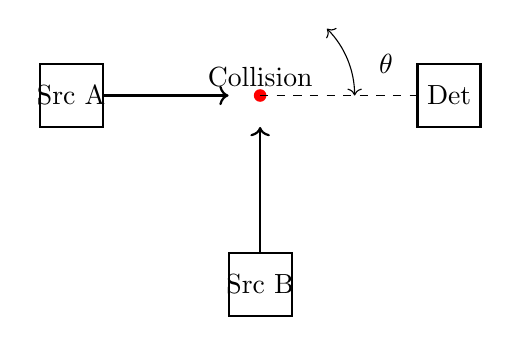
\begin{tikzpicture}[scale=0.8]
    % Source A
    \draw[thick] (-5,1) rectangle (-4,2);
    \node at (-4.5,1.5) {Src A};
    \draw[->, thick] (-4,1.5) -- (-2,1.5);

    % Source B
    \draw[thick] (-2,-2) rectangle (-1,-1);
    \node at (-1.5,-1.5) {Src B};
    \draw[->, thick] (-1.5,-1) -- (-1.5,1);

    % Collision Zone
    \fill[red] (-1.5,1.5) circle (0.1cm);
    \node at (-1.5,1.8) {Collision};

    % Detector
    \draw[thick] (1,1) rectangle (2,2);
    \node at (1.5,1.5) {Det};
    \draw[dashed] (-1.5,1.5) -- (1,1.5);
    \draw[<->] (0,1.5) arc (0:45:1.5);
    \node at (0.5,2) {$\theta$};
\end{tikzpicture}

\vspace{0.3cm}
\textbf{Components:}
\begin{itemize}
    \item \textbf{Sources:} Supersonic expansion (velocity selection)
    \item \textbf{Collision Zone:} Crossed beams at controlled angle
    \item \textbf{Detector:} Mass spectrometer + time-of-flight (TOF) analysis
    \item \textbf{Vacuum:} $10^{-6}$ to $10^{-8}$ torr to prevent multiple collisions
\end{itemize}

\end{frame}

% ===========================================================================
% Slide: Velocity Selection
% ===========================================================================
\begin{frame}{Velocity Selection: Supersonic Expansion}

\textbf{Technique:} Gas expands through small nozzle into vacuum

\begin{columns}[T]
\column{0.5\textwidth}
\textbf{Before Expansion:}
\begin{itemize}
    \item Maxwell-Boltzmann distribution
    \item $T \sim 300$ K
    \item Wide velocity spread
\end{itemize}

\vspace{0.3cm}
\textbf{After Expansion:}
\begin{itemize}
    \item Narrow velocity distribution
    \item Effective $T \sim 1$-$10$ K
    \item All molecules move with $v \approx \bar{v}$
\end{itemize}

\column{0.5\textwidth}
\centering
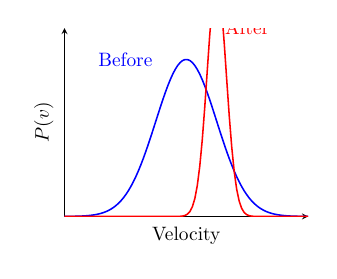
\begin{tikzpicture}[scale=0.7]
    \begin{axis}[
        xlabel={Velocity},
        ylabel={$P(v)$},
        xtick=\empty,
        ytick=\empty,
        axis lines=left,
        width=6cm,
        height=5cm,
        ymin=0, ymax=1.2
    ]
    % Broad distribution
    \addplot[blue, thick, domain=0:4, samples=100] {exp(-(x-2)^2/0.5)};
    \node[blue] at (axis cs:1,1) {Before};

    % Narrow distribution
    \addplot[red, thick, domain=0:4, samples=100] {1.5*exp(-(x-2.5)^2/0.05)};
    \node[red] at (axis cs:3,1.2) {After};
    \end{axis}
\end{tikzpicture}
\end{columns}

\textbf{Result:} Collision energy is well-defined!

\end{frame}

% ===========================================================================
% Slide: Collision Energy
% ===========================================================================
\begin{frame}{Collision Energy and Impact Parameter}

\textbf{Center-of-Mass Energy:}

For two molecules with velocities $\vec{v}_A$ and $\vec{v}_B$:

\keyeq{E_{\text{coll}} = \frac{1}{2}\mu v_{\text{rel}}^2}

where $\mu = \frac{m_A m_B}{m_A + m_B}$ is reduced mass.

\vspace{0.3cm}
\textbf{Impact Parameter $b$:}

\begin{columns}[T]
\column{0.6\textwidth}
\begin{itemize}
    \item Distance of closest approach if no interaction
    \item Small $b$: Head-on collision
    \item Large $b$: Grazing collision
    \item Maximum $b$ for reaction: $b_{\text{max}}$
    \item Reactive cross-section: $\sigma_r = \pi b_{\text{max}}^2$
\end{itemize}

\column{0.4\textwidth}
\centering
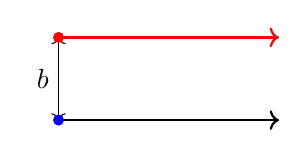
\begin{tikzpicture}[scale=0.7]
    \draw[->, thick] (0,0) -- (4,0);
    \draw[->, thick, red] (0,1.5) -- (4,1.5);
    \draw[<->] (0,0) -- (0,1.5) node[midway, left] {$b$};
    \fill[blue] (0,0) circle (0.1cm);
    \fill[red] (0,1.5) circle (0.1cm);
\end{tikzpicture}
\end{columns}

\end{frame}

% ===========================================================================
% Slide: Differential Cross-Section
% ===========================================================================
\begin{frame}{Differential Cross-Section}

\begin{columns}[T]
\column{0.55\textwidth}
\textbf{Definition:}

We measure the \textbf{Differential Cross-Section} $\sigma(\theta, \phi)$:

\keyeq{dN = \sigma(\theta, \phi) I_{\text{inc}} d\Omega}

\begin{itemize}
    \item $dN$: Particles scattered into $d\Omega$
    \item $I_{\text{inc}}$: Incident flux
    \item $\sigma(\theta)$: Angular cross-section
    \item Units: area/steradian (Å$^2$/sr)
\end{itemize}

\vspace{0.2cm}
\textbf{Information Content:}
\begin{itemize}
    \item Scattering probability vs angle
    \item Forces during collision
    \item Reaction mechanism
\end{itemize}

\column{0.45\textwidth}
\centering
\includegraphics[width=\textwidth]{Reaction_Dynamics_Interactive/images/differential_cross_section_polar.png}

\vspace{0.1cm}
\tiny \textit{Explore molecular beams interactively}

\end{columns}

\end{frame}

% ===========================================================================
% Slide: Scattering Patterns
% ===========================================================================
\begin{frame}{Types of Scattering Patterns}

\begin{columns}[T]
\column{0.5\textwidth}
\textbf{Forward Scattering ($\theta \approx 0°$):}
\begin{itemize}
    \item "Stripping" mechanism
    \item Grazing collision (large $b$)
    \item Fast, direct reaction
    \item Example: K + Br$_2$ → KBr + Br
    \item Products fly forward
\end{itemize}

\column{0.5\textwidth}
\textbf{Backward Scattering ($\theta \approx 180°$):}
\begin{itemize}
    \item "Rebound" mechanism
    \item Head-on collision (small $b$)
    \item Strong repulsive interaction
    \item Example: K + CH$_3$I
    \item Products bounce back
\end{itemize}
\end{columns}

\vspace{0.3cm}
\textbf{Sideways Scattering ($\theta \approx 90°$):}
\begin{itemize}
    \item Complex formation
    \item Long-lived intermediate
    \item Symmetric angular distribution
\end{itemize}

\end{frame}

% ===========================================================================
% Slide: Newton Diagram
% ===========================================================================
\begin{frame}{Newton Diagram}

\textbf{Relating Lab Frame to Center-of-Mass Frame:}

\begin{center}
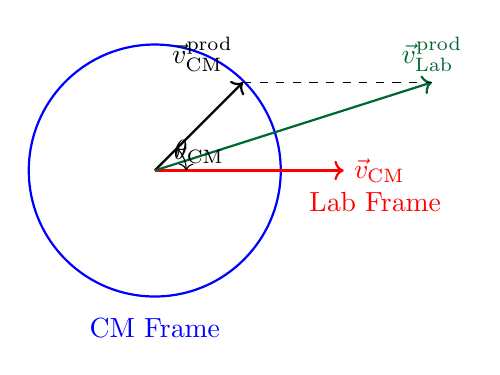
\begin{tikzpicture}[scale=0.8]
    % CM circle
    \draw[thick, blue] (0,0) circle (2cm);
    \node[blue] at (0,-2.5) {CM Frame};

    % Lab velocity
    \draw[->, thick, red] (0,0) -- (3,0) node[right] {$\vec{v}_{\text{CM}}$};
    \node[red] at (3.5,-0.5) {Lab Frame};

    % Product velocity in CM
    \draw[->, thick] (0,0) -- (1.4,1.4) node[above left] {$\vec{v}_{\text{CM}}^{\text{prod}}$};

    % Product velocity in Lab
    \draw[->, thick, darkgreen] (0,0) -- (4.4,1.4) node[above] {$\vec{v}_{\text{Lab}}^{\text{prod}}$};

    \draw[dashed] (1.4,1.4) -- (4.4,1.4);
    \draw[<->] (0.5,0) arc (0:45:0.5);
    \node at (0.7,0.3) {$\theta_{\text{CM}}$};
\end{tikzpicture}
\end{center}

\[ \vec{v}_{\text{Lab}} = \vec{v}_{\text{CM}}^{\text{prod}} + \vec{v}_{\text{CM}} \]

Detector measures lab angles; theory predicts CM angles.

\end{frame}

% ===========================================================================
% Slide: State-to-State Chemistry - Part 1
% ===========================================================================
\begin{frame}{State-to-State Chemistry (Part 1)}

\textbf{Modern Achievement:} Prepare reactants in specific quantum states and measure product states.

\vspace{0.5cm}
\textbf{Example:} H + D$_2$(v=0, J=0) → HD(v', J') + D

\begin{itemize}
    \item Prepare D$_2$ in ground vibrational and rotational state
    \item Measure HD product distribution over v' and J'
    \item Map out complete energy disposal
\end{itemize}

\vspace{0.5cm}
\textbf{Advantages:}
\begin{itemize}
    \item Most detailed information possible
    \item Direct test of theory
    \item Reveals quantum effects
\end{itemize}

\end{frame}

% ===========================================================================
% Slide: State-to-State Chemistry - Part 2
% ===========================================================================
\begin{frame}{State-to-State Chemistry (Part 2)}

\textbf{Experimental Techniques:}
\begin{itemize}
    \item \textbf{State preparation:} Laser excitation, Stark/Zeeman selection
    \item \textbf{State detection:} Laser-induced fluorescence (LIF), REMPI
\end{itemize}

\vspace{0.5cm}
\textbf{Ultimate Goal:} Complete characterization:
\[ \sigma(E_{\text{coll}}, v, J, b \to v', J', \theta, \phi) \]

This is the \alert{full quantum scattering matrix}!

\vspace{0.5cm}
\textbf{Challenge:} Enormous amount of data, but worth it for fundamental understanding

\end{frame}

% ===========================================================================
% Slide: Potential Energy Surfaces (PES)
% ===========================================================================
\begin{frame}{Potential Energy Surfaces (PES)}

\textbf{The Landscape of Reaction}

\begin{itemize}
    \item Plot Potential Energy $V$ vs. atomic coordinates.
    \item For A + BC $\to$ AB + C (collinear):
        \item Axes: $R_{AB}$ and $R_{BC}$.
\end{itemize}

\vspace{0.2cm}
\centering
\includegraphics[width=0.7\textwidth]{Reaction_Dynamics_Interactive/images/pes_contour_leps.png}

\vspace{0.1cm}
{\small LEPS Potential Energy Surface for A + BC $\to$ AB + C}

\vspace{0.1cm}
\textbf{Reality:} 3N-6 dimensions for N atoms (reduced to 2D for collinear triatomics)

\end{frame}

% ===========================================================================
% Slide: Calculating PES - Part 1
% ===========================================================================
\begin{frame}{How to Calculate PES (Part 1)}

\textbf{Theoretical Methods:}

\begin{enumerate}
    \item \textbf{Ab Initio Quantum Chemistry:}
        \begin{itemize}
            \item Solve Schrödinger equation for electrons
            \item Born-Oppenheimer approximation (nuclei fixed)
            \item Methods: HF, MP2, CCSD(T), CASSCF
            \item Very accurate but computationally expensive
        \end{itemize}

    \item \textbf{Density Functional Theory (DFT):}
        \begin{itemize}
            \item Faster than ab initio
            \item Good accuracy for many systems
            \item Functionals: B3LYP, M06-2X, $\omega$B97X-D
        \end{itemize}
\end{enumerate}

\end{frame}

% ===========================================================================
% Slide: Calculating PES - Part 2
% ===========================================================================
\begin{frame}{How to Calculate PES (Part 2)}

\textbf{Theoretical Methods (continued):}

\begin{enumerate}
    \setcounter{enumi}{2}
    \item \textbf{Semi-Empirical/Fitted:}
        \begin{itemize}
            \item LEPS (London-Eyring-Polanyi-Sato)
            \item Fit to experimental data
            \item Fast but less accurate
        \end{itemize}
\end{enumerate}

\vspace{0.5cm}
\textbf{Trade-offs:}
\begin{itemize}
    \item Accuracy vs. computational cost
    \item Ab initio: Most accurate, most expensive
    \item DFT: Good balance for most systems
    \item Semi-empirical: Fast screening, less reliable
\end{itemize}

\end{frame}

% ===========================================================================
% Slide: Features of PES
% ===========================================================================
\begin{frame}{Features of PES}

\begin{columns}[T]
\column{0.5\textwidth}
\begin{itemize}
    \item \textbf{Reactant Valley:} A far from BC.
    \item \textbf{Product Valley:} AB far from C.
    \item \textbf{Saddle Point:} The Transition State.
        \item Maximum along reaction path.
        \item Minimum perpendicular to path.
    \item \textbf{Reaction Path:} Minimum energy route (MEP).
    \item \textbf{Barrier Height:} Energy at saddle point.
\end{itemize}

\column{0.5\textwidth}
\centering
% Simplified diagram
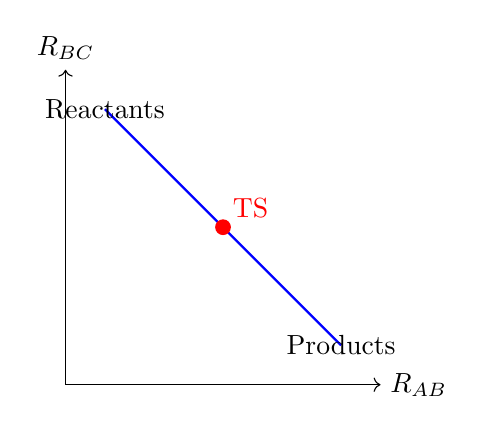
\begin{tikzpicture}
    \draw[->] (0,0) -- (4,0) node[right] {$R_{AB}$};
    \draw[->] (0,0) -- (0,4) node[above] {$R_{BC}$};
    \draw[thick, blue] (0.5,3.5) to[out=-45,in=135] (3.5,0.5);
    \node at (0.5,3.5) {Reactants};
    \node at (3.5,0.5) {Products};
    \fill[red] (2,2) circle (0.1cm) node[above right] {TS};
\end{tikzpicture}
\end{columns}

\vspace{0.3cm}
\textbf{Intrinsic Reaction Coordinate (IRC):} Path of steepest descent from TS to reactants and products.

\end{frame}

% ===========================================================================
% Slide: Classical Trajectories - Part 1
% ===========================================================================
\begin{frame}{Classical Trajectory Calculations (Part 1)}

\textbf{Method:} Solve Newton's equations on the PES

\begin{enumerate}
    \item Start with initial conditions: positions, velocities, $E_{\text{coll}}$, $b$
    \item Calculate forces: $\vec{F}_i = -\nabla_i V(\vec{R})$
    \item Integrate equations of motion: $m_i \ddot{\vec{R}}_i = \vec{F}_i$
    \item Follow trajectory until products separate
    \item Record: reaction outcome, scattering angle, product energies
\end{enumerate}

\end{frame}

% ===========================================================================
% Slide: Classical Trajectories - Part 2
% ===========================================================================
\begin{frame}{Classical Trajectory Calculations (Part 2)}

\textbf{Statistical Analysis:}
\begin{itemize}
    \item Run thousands of trajectories
    \item Sample different $b$ and initial conditions
    \item Calculate average cross-sections, energy distributions
\end{itemize}

\vspace{0.5cm}
\textbf{Limitations:}
\begin{itemize}
    \item Classical mechanics (no tunneling)
    \item Can violate zero-point energy (ZPE)
    \item No quantum interference effects
    \item Need ZPE constraints for realistic simulations
\end{itemize}

\vspace{0.5cm}
\textbf{When to use:} Heavy atoms, high energies, statistical averaging

\end{frame}

% ===========================================================================
% Slide: Trajectory Example
% ===========================================================================
\begin{frame}{Trajectory Example: H + H$_2$ → H$_2$ + H}

\begin{center}
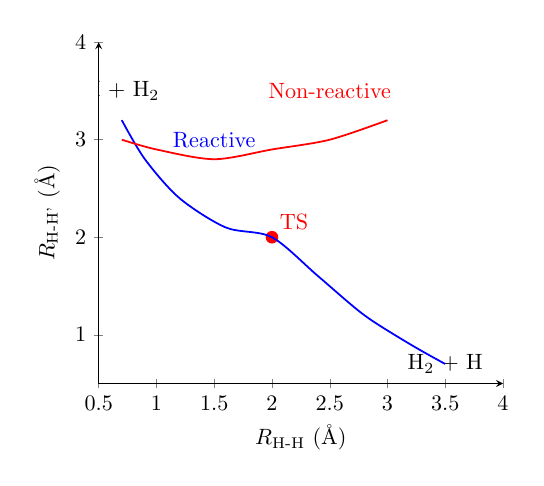
\begin{tikzpicture}[scale=0.8]
    \begin{axis}[
        xlabel={$R_{\text{H-H}}$ (Å)},
        ylabel={$R_{\text{H-H'}}$ (Å)},
        xmin=0.5, xmax=4,
        ymin=0.5, ymax=4,
        axis lines=left,
        width=8cm,
        height=7cm
    ]
    % Reactant valley
    \node at (axis cs:0.7,3.5) {H + H$_2$};
    % Product valley
    \node at (axis cs:3.5,0.7) {H$_2$ + H};
    % TS region
    \fill[red] (axis cs:2,2) circle (0.1cm) node[above right] {TS};

    % Reactive trajectory
    \addplot[blue, thick, smooth] coordinates {
        (0.7,3.2) (0.9,2.8) (1.2,2.4) (1.6,2.1) (2.0,2.0) (2.4,1.6) (2.8,1.2) (3.2,0.9) (3.5,0.7)
    };
    \node[blue] at (axis cs:1.5,3) {Reactive};

    % Non-reactive trajectory
    \addplot[red, thick, smooth] coordinates {
        (0.7,3.0) (1.0,2.9) (1.5,2.8) (2.0,2.9) (2.5,3.0) (3.0,3.2)
    };
    \node[red] at (axis cs:2.5,3.5) {Non-reactive};
    \end{axis}
\end{tikzpicture}
\end{center}

Blue: Passes through TS region → reaction. Red: Turns back → no reaction.

\end{frame}

% ===========================================================================
% Slide: Product Energy Distribution
% ===========================================================================
\begin{frame}{Product Energy Distribution}

\textbf{Where does the energy go?}

Total available energy: $E_{\text{avail}} = E_{\text{coll}} + \Delta H_{\text{rxn}}$

\textbf{Partitioning:}
\begin{itemize}
    \item \textbf{Translation:} $E_{\text{trans}}$ (kinetic energy of products flying apart)
    \item \textbf{Vibration:} $E_{\text{vib}}$ (internal vibration of product molecules)
    \item \textbf{Rotation:} $E_{\text{rot}}$ (molecular rotation)
\end{itemize}

\keyeq{E_{\text{avail}} = E_{\text{trans}} + E_{\text{vib}} + E_{\text{rot}}}

\vspace{0.3cm}
\textbf{Distribution depends on PES topology:}
\begin{itemize}
    \item Attractive surface → vibrationally "hot" products
    \item Repulsive surface → translationally "hot" products
\end{itemize}

\end{frame}

% ===========================================================================
% Slide: Attractive vs. Repulsive Surfaces
% ===========================================================================
\begin{frame}{Attractive vs. Repulsive Surfaces}

\textbf{Where is the barrier located?}

\begin{columns}[T]
\column{0.5\textwidth}
\textbf{Attractive (Early Barrier):}
\begin{itemize}
    \item Barrier in reactant valley
    \item TS resembles reactants
    \item \alert{Translational energy} helps cross barrier
    \item Products are \alert{vibrationally excited}
    \item Example: K + Br$_2$ (Harpoon reaction)
    \item Energy flows: Translation → Vibration
\end{itemize}

\column{0.5\textwidth}
\textbf{Repulsive (Late Barrier):}
\begin{itemize}
    \item Barrier in product valley
    \item TS resembles products
    \item \alert{Vibrational energy} helps cross barrier
    \item Products are \alert{translationally excited}
    \item Example: H + Cl$_2$
    \item Energy flows: Vibration → Translation
\end{itemize}
\end{columns}

\end{frame}

% ===========================================================================
% Slide: Polanyi's Rules - Part 1
% ===========================================================================
\begin{frame}{Polanyi's Rules (Part 1)}

\emphbox{
\textbf{Polanyi's Rule 1:} For reactions with early barriers, translational energy is more effective than vibrational energy in promoting reaction.
}

\emphbox{
\textbf{Polanyi's Rule 2:} For reactions with late barriers, vibrational energy is more effective than translational energy in promoting reaction.
}

\vspace{0.5cm}
\textbf{Key Insight:} The location of the barrier determines which type of energy is most effective.

\end{frame}

% ===========================================================================
% Slide: Polanyi's Rules - Part 2
% ===========================================================================
\begin{frame}{Polanyi's Rules (Part 2)}

\textbf{Intuitive Explanation:}
\begin{itemize}
    \item \textbf{Early Barrier:} Need speed to "run up" the entrance valley before bonds rearrange.
    \item \textbf{Late Barrier:} Need stretched bonds (vibration) to help make the turn into the product valley.
\end{itemize}

\vspace{0.5cm}
\textbf{Experimental Verification:}
\begin{itemize}
    \item Compare $\sigma_r(E_{\text{trans}}, v=0)$ vs. $\sigma_r(E_{\text{trans}}, v=1)$
    \item Prepare reactants with vibrational excitation
    \item Measure which form of energy enhances reactivity more
\end{itemize}

\vspace{0.5cm}
\textbf{Impact:} Guide for controlling chemical reactions with laser excitation

\end{frame}

% ===========================================================================
% Slide: Energy Disposal
% ===========================================================================
\begin{frame}{Energy Disposal: Surprisal Analysis}

\textbf{Question:} How does actual product energy distribution compare to statistical expectation?

\textbf{Statistical (Phase Space) Prediction:}
\begin{itemize}
    \item Assume all product states equally accessible
    \item Predict: $P_{\text{stat}}(v') \propto \rho(E_{\text{avail}} - E_{v'})$
    \item Density of states $\rho$ increases with energy
\end{itemize}

\vspace{0.3cm}
\textbf{Surprisal:}
\keyeq{I(v') = -\ln\left(\frac{P_{\text{obs}}(v')}{P_{\text{stat}}(v')}\right)}

\begin{itemize}
    \item $I(v') > 0$: Less than statistical (vibration "starved")
    \item $I(v') < 0$: More than statistical (vibration "enhanced")
\end{itemize}

\textbf{Reveals:} Direct vs. complex mechanism

\end{frame}

% ===========================================================================
% Slide: Harpoon Mechanism - Part 1
% ===========================================================================
\begin{frame}{Harpoon Mechanism: K + Br$_2$ → KBr + Br (Part 1)}

\textbf{Classic Example of Attractive Surface}

\vspace{0.3cm}
\textbf{Mechanism:}
\begin{enumerate}
    \item At large distance ($R \sim 6$ Å): Electron jumps from K to Br$_2$
        \[ \text{K} + \text{Br}_2 \to \text{K}^+ + \text{Br}_2^- \]
    \item Coulomb attraction pulls ions together (fast!)
    \item K$^+$ approaches Br$_2^-$, forming KBr$^-$ complex
    \item Br$^-$ leaves with high kinetic energy
\end{enumerate}

\end{frame}

% ===========================================================================
% Slide: Harpoon Mechanism - Part 2
% ===========================================================================
\begin{frame}{Harpoon Mechanism: K + Br$_2$ → KBr + Br (Part 2)}

\textbf{Experimental Observations:}
\begin{itemize}
    \item Very large cross-section: $\sigma \sim 200$ Å$^2$ (vs. $\sim 10$ Å$^2$ typical)
    \item Forward scattering (stripping mechanism)
    \item KBr product highly vibrationally excited
    \item Low activation energy
\end{itemize}

\vspace{0.5cm}
\textbf{Why "Harpoon"?}
\begin{itemize}
    \item Electron "thrown" from K at long range
    \item Like harpooning a whale from distance
    \item Ionic attraction then "reels in" the reactants
    \item Fast, efficient reaction
\end{itemize}

\end{frame}

% ===========================================================================
% Slide: Spectator Stripping
% ===========================================================================
\begin{frame}{Spectator Stripping}

\textbf{Mechanism:} In A + BC → AB + C, atom C is a "spectator"

\begin{columns}[T]
\column{0.6\textwidth}
\textbf{Characteristics:}
\begin{itemize}
    \item Fast, direct reaction
    \item C atom barely affected
    \item AB bond forms while BC bond breaks
    \item High impact parameter (grazing collision)
    \item Forward scattering
    \item C "stripped off" from BC
\end{itemize}

\vspace{0.3cm}
\textbf{Example:} K + CH$_3$I → KI + CH$_3$
\begin{itemize}
    \item CH$_3$ group acts as spectator
    \item KI formed in collision zone
    \item CH$_3$ continues forward with little deflection
\end{itemize}

\column{0.4\textwidth}
\centering
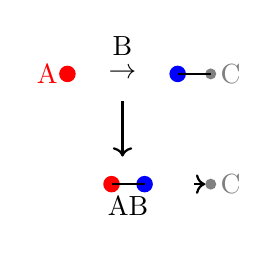
\begin{tikzpicture}[scale=0.7]
    % Before
    \fill[red] (0,2) circle (0.15cm) node[left] {A};
    \fill[blue] (2,2) circle (0.15cm);
    \fill[gray] (2.6,2) circle (0.1cm) node[right] {C};
    \draw[thick] (2,2) -- (2.6,2);
    \node at (1,2) {$\to$};
    \node at (1,2.5) {B};

    % Arrow
    \draw[->, thick] (1,1.5) -- (1,0.5);

    % After
    \fill[red] (0.8,0) circle (0.15cm);
    \fill[blue] (1.4,0) circle (0.15cm);
    \draw[thick] (0.8,0) -- (1.4,0);
    \node at (1.1,-0.4) {AB};

    \fill[gray] (2.6,0) circle (0.1cm) node[right] {C};
    \draw[->, thick] (2.3,0) -- (2.5,0);
\end{tikzpicture}
\end{columns}

\end{frame}

% ===========================================================================
% Slide: Quantum Effects - Part 1
% ===========================================================================
\begin{frame}{Quantum Effects in Dynamics (Part 1)}

\textbf{When Classical Trajectories Fail:}

\begin{enumerate}
    \item \textbf{Tunneling:}
        \begin{itemize}
            \item Light atoms (H, D) can tunnel through barriers
            \item Important for H-transfer reactions
            \item Classical: $k = 0$ below barrier; Quantum: $k > 0$
        \end{itemize}

    \item \textbf{Zero-Point Energy (ZPE):}
        \begin{itemize}
            \item Molecules have ZPE = $\frac{1}{2}h\nu$ even at $v=0$
            \item Classical trajectories can violate ZPE
            \item Need ZPE constraints in classical simulations
        \end{itemize}
\end{enumerate}

\end{frame}

% ===========================================================================
% Slide: Quantum Effects - Part 2
% ===========================================================================
\begin{frame}{Quantum Effects in Dynamics (Part 2)}

\textbf{When Classical Trajectories Fail (continued):}

\begin{enumerate}
    \setcounter{enumi}{2}
    \item \textbf{Resonances:}
        \begin{itemize}
            \item Quasi-bound states in complex region
            \item Show up as oscillations in $\sigma_r(E)$
            \item Pure quantum effect (interference)
        \end{itemize}

    \item \textbf{Quantized Product States:}
        \begin{itemize}
            \item Classical: continuous energy distribution
            \item Quantum: discrete vibrational/rotational levels
        \end{itemize}
\end{enumerate}

\vspace{0.5cm}
\textbf{Bottom Line:} Quantum dynamics needed for light atoms, low energies, or detailed state-to-state studies.

\end{frame}

% ===========================================================================
% Slide: Worked Example 1
% ===========================================================================
\begin{frame}{Worked Example 1: Collision Energy}

\textbf{Problem:} In a crossed molecular beam experiment, H atoms (mass = 1 amu) with velocity 2000 m/s collide with D$_2$ molecules (mass = 4 amu) at rest. Calculate the collision energy.

\vspace{0.3cm}
\textbf{Solution:}

Step 1: Calculate reduced mass
\[ \mu = \frac{m_{\text{H}} \cdot m_{\text{D}_2}}{m_{\text{H}} + m_{\text{D}_2}} = \frac{1 \times 4}{1 + 4} = 0.8 \text{ amu} \]

Convert to kg: $\mu = 0.8 \times 1.66 \times 10^{-27} = 1.33 \times 10^{-27}$ kg

Step 2: Relative velocity
\[ v_{\text{rel}} = v_{\text{H}} - v_{\text{D}_2} = 2000 - 0 = 2000 \text{ m/s} \]

Step 3: Collision energy
\[ E_{\text{coll}} = \frac{1}{2}\mu v_{\text{rel}}^2 = \frac{1}{2}(1.33 \times 10^{-27})(2000)^2 = 2.66 \times 10^{-21} \text{ J} \]

\keyeq{E_{\text{coll}} = 0.016 \text{ eV} = 1.55 \text{ kJ/mol}}

\end{frame}

% ===========================================================================
% Slide: Worked Example 2
% ===========================================================================
\begin{frame}{Worked Example 2: Reactive Cross-Section}

\textbf{Problem:} For the reaction H + D$_2$ → HD + D, the maximum impact parameter for reaction at $E_{\text{coll}} = 0.5$ eV is $b_{\text{max}} = 1.8$ Å. Calculate:
\begin{enumerate}[a)]
    \item The reactive cross-section $\sigma_r$
    \item The reaction probability if geometric cross-section is $\sigma_{\text{geom}} = 10$ Å$^2$
\end{enumerate}

\vspace{0.3cm}
\textbf{Solution:}

(a) Reactive cross-section:
\[ \sigma_r = \pi b_{\text{max}}^2 = \pi (1.8)^2 = 10.2 \text{ Å}^2 \]

(b) Reaction probability (opacity function):
\[ P = \frac{\sigma_r}{\sigma_{\text{geom}}} = \frac{10.2}{10} = 1.02 \approx 1.0 \]

\textbf{Interpretation:} At this energy, essentially all collisions within the geometric cross-section lead to reaction (high reactivity).

\end{frame}

% ===========================================================================
% Slide: Worked Example 3
% ===========================================================================
\begin{frame}{Worked Example 3: Energy Partitioning}

\textbf{Problem:} For the reaction F + H$_2$ → HF + H at $E_{\text{coll}} = 0.1$ eV:
\begin{itemize}
    \item $\Delta H_{\text{rxn}} = -1.4$ eV (exothermic)
    \item Measured: HF products have $\langle E_{\text{vib}} \rangle = 1.0$ eV
\end{itemize}

Calculate the average translational and rotational energy of products.

\vspace{0.3cm}
\textbf{Solution:}

Total available energy:
\[ E_{\text{avail}} = E_{\text{coll}} + |\Delta H_{\text{rxn}}| = 0.1 + 1.4 = 1.5 \text{ eV} \]

Energy remaining for translation + rotation:
\[ E_{\text{trans}} + E_{\text{rot}} = E_{\text{avail}} - E_{\text{vib}} = 1.5 - 1.0 = 0.5 \text{ eV} \]

Typical ratio: $E_{\text{rot}} : E_{\text{trans}} \approx 1:2$ (rule of thumb)

\keyeq{E_{\text{rot}} \approx 0.17 \text{ eV}, \quad E_{\text{trans}} \approx 0.33 \text{ eV}}

\textbf{Note:} HF is highly vibrationally excited (67\% into vibration) - characteristic of attractive surface.

\end{frame}

% ===========================================================================
% Slide: Practice Problem 1
% ===========================================================================
\begin{frame}{Practice Problem 1}

\textbf{Problem:} In a crossed beam experiment, Ar atoms (40 amu) with $v = 1500$ m/s collide with O$_2$ molecules (32 amu) with $v = 800$ m/s at 90°. Calculate:

\begin{enumerate}[a)]
    \item The magnitude of the relative velocity
    \item The collision energy in eV
    \item The center-of-mass velocity
\end{enumerate}

\vspace{0.5cm}
\textbf{Answers:}
\begin{itemize}
    \item[(a)] $v_{\text{rel}} = \sqrt{1500^2 + 800^2} = 1700$ m/s
    \item[(b)] $E_{\text{coll}} = 0.17$ eV
    \item[(c)] $v_{\text{CM}} = 1056$ m/s (along Ar beam direction)
\end{itemize}

\end{frame}

% ===========================================================================
% Slide: Practice Problem 2
% ===========================================================================
\begin{frame}{Practice Problem 2}

\textbf{Problem:} For the reaction Cl + HBr → HCl + Br:
\begin{itemize}
    \item Barrier is "late" (in product valley)
    \item $E_a = 8$ kJ/mol
\end{itemize}

\begin{enumerate}[a)]
    \item According to Polanyi's rules, would vibrational or translational energy be more effective?
    \item If HBr has vibrational energy 25 kJ/mol, estimate the effective activation energy.
    \item Predict whether products will be vibrationally or translationally "hot".
\end{enumerate}

\vspace{0.3cm}
\textbf{Answers:}
\begin{itemize}
    \item[(a)] Vibrational energy (late barrier)
    \item[(b)] $E_a^{\text{eff}} \approx 8 - 0.3(25) \approx 0.5$ kJ/mol (much lower!)
    \item[(c)] Products will be translationally hot (repulsive surface)
\end{itemize}

\end{frame}

% ===========================================================================
% Slide: Practice Problem 3
% ===========================================================================
\begin{frame}{Practice Problem 3}

\textbf{Problem:} A reaction has measured differential cross-section:
\[ \sigma(\theta) = \sigma_0 \cos^2(\theta) \]

where $\sigma_0 = 15$ Å$^2$/sr.

\begin{enumerate}[a)]
    \item Sketch the angular distribution
    \item Is this forward or backward scattering?
    \item What mechanism does this suggest?
    \item Calculate the total cross-section: $\sigma_{\text{total}} = \int \sigma(\theta) d\Omega$
\end{enumerate}

\vspace{0.3cm}
\textbf{Answers:}
\begin{itemize}
    \item[(a)] Maximum at $\theta = 0°$ and $180°$, zero at $90°$
    \item[(b)] Both forward and backward (symmetric)
    \item[(c)] Head-on collision with rebound
    \item[(d)] $\sigma_{\text{total}} = 20\pi$ Å$^2 \approx 63$ Å$^2$
\end{itemize}

\end{frame}

% ===========================================================================
% Slide: Practice Problem 4
% ===========================================================================
\begin{frame}{Practice Problem 4}

\textbf{Problem:} For H + H$_2$ → H$_2$ + H reaction:
\begin{itemize}
    \item Classical barrier: $E_a^{\text{classical}} = 40$ kJ/mol
    \item Measured barrier: $E_a^{\text{obs}} = 32$ kJ/mol
\end{itemize}

\begin{enumerate}[a)]
    \item What causes the difference?
    \item Estimate the effective tunneling distance if the barrier width is 0.5 Å
    \item Would the isotopic reaction D + D$_2$ → D$_2$ + D show a larger or smaller difference?
\end{enumerate}

\vspace{0.3cm}
\textbf{Answers:}
\begin{itemize}
    \item[(a)] Quantum tunneling through the barrier
    \item[(b)] Tunneling reduces effective barrier by $\sim 8$ kJ/mol (20\%)
    \item[(c)] Smaller difference - heavier mass reduces tunneling probability:
    \[ P_{\text{tunnel}} \propto \exp(-\sqrt{2m\Delta E} \cdot d/\hbar) \]
\end{itemize}

\end{frame}

% ===========================================================================
% Slide: Modern Developments - Part 1
% ===========================================================================
\begin{frame}{Modern Developments in Reaction Dynamics (Part 1)}

\textbf{Cutting Edge Techniques:}

\begin{enumerate}
    \item \textbf{Femtochemistry (A. Zewail, Nobel 1999):}
        \begin{itemize}
            \item Femtosecond laser pulses ($10^{-15}$ s)
            \item Watch bonds break and form in real time
            \item "Molecular movies" of reactions
        \end{itemize}

    \item \textbf{Coulomb Explosion Imaging:}
        \begin{itemize}
            \item Remove all electrons instantly
            \item Nuclei fly apart by Coulomb repulsion
            \item Measure 3D structure at instant of explosion
        \end{itemize}
\end{enumerate}

\end{frame}

% ===========================================================================
% Slide: Modern Developments - Part 2
% ===========================================================================
\begin{frame}{Modern Developments in Reaction Dynamics (Part 2)}

\textbf{Cutting Edge Techniques (continued):}

\begin{enumerate}
    \setcounter{enumi}{2}
    \item \textbf{Cold Molecule Chemistry:}
        \begin{itemize}
            \item Molecules cooled to $\mu$K with lasers
            \item Study reactions at ultralow energies
            \item Quantum effects dominate
        \end{itemize}

    \item \textbf{High-Dimensional Quantum Dynamics:}
        \begin{itemize}
            \item Beyond 3-atom systems
            \item Full quantum treatment of 4-, 5-, 6-atom reactions
            \item Enables prediction without experiments
        \end{itemize}
\end{enumerate}

\vspace{0.5cm}
\textbf{Impact:} From "what happens" to "why and how" at atomic resolution

\end{frame}

% ===========================================================================
% Slide: Summary Topic 18D
% ===========================================================================
\begin{frame}{Summary: Topic 18D}

\begin{enumerate}
    \item \textbf{Molecular Beams:} Enable study of single collisions with controlled conditions
        \begin{itemize}
            \item State selection, velocity control, angular resolution
        \end{itemize}

    \item \textbf{Differential Cross-Sections:} Reveal reaction mechanisms
        \begin{itemize}
            \item Forward: stripping; Backward: rebound; Sideways: complex
        \end{itemize}

    \item \textbf{Potential Energy Surfaces:} Map of reaction landscape
        \begin{itemize}
            \item Calculated from quantum chemistry
            \item Used for trajectory calculations
        \end{itemize}

    \item \textbf{Energy Distribution:} Not statistical!
        \begin{itemize}
            \item Attractive surface → vibrationally hot products
            \item Repulsive surface → translationally hot products
        \end{itemize}

    \item \textbf{Polanyi's Rules:} Connect barrier location to energy requirements
        \begin{itemize}
            \item Early barrier: translation promotes; Late barrier: vibration promotes
        \end{itemize}
\end{enumerate}

\end{frame}

% ===========================================================================
% Slide: Interactive Resources for Topic 18D
% ===========================================================================
\begin{frame}{Interactive Learning: Topic 18D}

\begin{columns}[c]
\column{0.65\textwidth}
\textbf{Explore Molecular Collision Dynamics Interactively!}

\vspace{0.3cm}

\textbf{Interactive Jupyter Notebook Features:}
\begin{itemize}
    \item \textbf{3D PES Visualizer}: Rotate and explore potential surfaces
    \item \textbf{Trajectory Simulator}: Watch reactive vs non-reactive paths
    \item \textbf{Molecular Beam Setup}: Understand crossed-beam experiments
    \item \textbf{Differential Cross-Section}: Analyze angular distributions
    \item \textbf{Newton Diagrams}: Product velocity vectors
    \item \textbf{State-to-State Dynamics}: Quantum state resolution
\end{itemize}

\vspace{0.3cm}

\textbf{Notebook:} \texttt{04\_Molecular\_Dynamics.ipynb}

\column{0.35\textwidth}
\centering
\textbf{Scan to Open:}

\vspace{0.3cm}

\includegraphics[width=0.8\textwidth]{QR_codes/04_Molecular_Dynamics.png}

\vspace{0.3cm}

{\footnotesize Or navigate to:\\
\texttt{Reaction\_Dynamics\_Interactive/}}

\end{columns}

\end{frame}


% ============================================================================
% TOPIC 18E: ELECTRON TRANSFER
% ============================================================================

\section{Topic 18E: Electron Transfer}

% ===========================================================================
% Slide: Topic 18E Overview
% ===========================================================================
\begin{frame}{Topic 18E: Overview}

\textbf{Electron Transfer (ET) Reactions}

\[ \ch{D + A -> D^+ + A^-} \]

\vspace{0.3cm}
\begin{itemize}
    \item \textbf{Simplest} class of reactions: just electron movement
    \item No bonds broken or formed in elementary step
    \item Ubiquitous in chemistry, biology, materials science
    \item \textbf{Marcus Theory:} Rudolph Marcus, Nobel Prize 1992
\end{itemize}

\vspace{0.3cm}
\textbf{Examples:}
\begin{itemize}
    \item \textbf{Biology:} Photosynthesis, respiration (cytochrome chains)
    \item \textbf{Chemistry:} Redox reactions, fuel cells, batteries
    \item \textbf{Materials:} Organic electronics, solar cells
\end{itemize}

\end{frame}

% ===========================================================================
% Slide: Types of Electron Transfer - Part 1
% ===========================================================================
\begin{frame}{Types of Electron Transfer Reactions (Part 1)}

\textbf{1. Self-Exchange Reactions:}
\[ \ch{Fe^{2+} + Fe^{3+} -> Fe^{3+} + Fe^{2+}} \]
\begin{itemize}
    \item $\Delta_r G^\circ = 0$ (no driving force)
    \item Rate depends only on reorganization energy
    \item Used to measure intrinsic barrier
\end{itemize}

\vspace{0.5cm}
\textbf{2. Cross Reactions:}
\[ \ch{D + A -> D^+ + A^-} \]
\begin{itemize}
    \item $\Delta_r G^\circ \neq 0$
    \item Thermodynamically driven
    \item Rate depends on driving force AND reorganization
\end{itemize}

\end{frame}

% ===========================================================================
% Slide: Types of Electron Transfer - Part 2
% ===========================================================================
\begin{frame}{Types of Electron Transfer Reactions (Part 2)}

\textbf{3. Inner vs. Outer Sphere:}
\begin{itemize}
    \item \textbf{Outer Sphere:} Electron tunnels, no ligand exchange
    \item \textbf{Inner Sphere:} Bridge ligand shared, chemical bond formation
\end{itemize}

\vspace{0.5cm}
\textbf{Comparison:}
\begin{itemize}
    \item Outer sphere: Simple, predictable by Marcus theory
    \item Inner sphere: More complex, involves bond making/breaking
    \item Most biological ET is outer sphere
    \item Transition metal chemistry has both types
\end{itemize}

\end{frame}

% ===========================================================================
% Slide: Thermodynamics of ET
% ===========================================================================
\begin{frame}{Thermodynamics of Electron Transfer}

\textbf{Driving Force:} Determined by reduction potentials

For: \ch{D + A -> D^+ + A^-}

\keyeq{\Delta_r G^\circ = -F(E_{\text{D}^+/\text{D}} - E_{\text{A}/\text{A}^-})}

where $F$ is Faraday constant (96485 C/mol).

\vspace{0.3cm}
\textbf{Example:}
\begin{itemize}
    \item \ch{Ru(bpy)_3^{2+}} (D): $E^\circ = -1.3$ V vs. NHE
    \item \ch{MV^{2+}} (A): $E^\circ = -0.45$ V vs. NHE
    \item $\Delta_r G^\circ = -F(-1.3 - (-0.45)) = -F(-0.85) = +82$ kJ/mol
\end{itemize}

Positive $\Delta_r G^\circ$ → endergonic, need excitation.

\end{frame}

% ===========================================================================
% Slide: The Franck-Condon Principle
% ===========================================================================
\begin{frame}{The Franck-Condon Principle}

\textbf{Key Concept:} Electrons move \alert{much faster} than nuclei.

\begin{itemize}
    \item Electron transfer time: $\sim 10^{-15}$ s (femtoseconds)
    \item Nuclear motion time: $\sim 10^{-13}$ s (100 fs)
\end{itemize}

\vspace{0.3cm}
\emphbox{
\textbf{Franck-Condon Principle:} Electron transfer occurs at \alert{fixed nuclear geometry} - a "vertical" transition on energy diagram.
}

\vspace{0.3cm}
\textbf{Consequences:}
\begin{itemize}
    \item Energy must be conserved at the instant of transfer
    \item Reactant and product energy surfaces must intersect
    \item Nuclei must reorganize \textit{before} electron jumps
    \item Reorganization creates activation barrier
\end{itemize}

\end{frame}

% ===========================================================================
% Slide: Potential Energy Surfaces
% ===========================================================================
\begin{frame}{Potential Energy Surfaces for ET}

\centering
\includegraphics[width=0.8\textwidth]{Reaction_Dynamics_Interactive/images/marcus_parabolas_annotated.png}

\vspace{0.2cm}
\textbf{Reorganization energy $\lambda$:} Vertical distance from product minimum to reactant curve.

\vspace{0.1cm}
\tiny \textit{Interactive Marcus theory explorer available in notebook}

\end{frame}

% ===========================================================================
% Slide: Reorganization Energy Components
% ===========================================================================
\begin{frame}{Reorganization Energy ($\lambda$)}

\textbf{Total reorganization energy:}
\keyeq{\lambda = \lambda_{\text{in}} + \lambda_{\text{out}}}

\vspace{0.3cm}
\textbf{1. Inner Sphere ($\lambda_{\text{in}}$):}
\begin{itemize}
    \item Changes in bond lengths and angles of D and A
    \item Example: Fe$^{2+}$ has longer bonds than Fe$^{3+}$
    \item Typical: 0.2-1.0 eV for transition metal complexes
    \item Small for organic molecules with delocalized $\pi$ systems
\end{itemize}

\vspace{0.3cm}
\textbf{2. Outer Sphere ($\lambda_{\text{out}}$):}
\begin{itemize}
    \item Reorientation of solvent molecules
    \item Ions polarize solvent differently
    \item Depends on: solvent dielectric constant, ion size
    \item Typical: 0.5-1.5 eV in polar solvents
\end{itemize}

\end{frame}

% ===========================================================================
% Slide: Calculating Outer Sphere λ
% ===========================================================================
\begin{frame}{Marcus Formula for $\lambda_{\text{out}}$}

\textbf{Dielectric Continuum Model:}

\keyeq{\lambda_{\text{out}} = \frac{e^2}{4\pi\varepsilon_0}\left(\frac{1}{2r_D} + \frac{1}{2r_A} - \frac{1}{d}\right)\left(\frac{1}{\varepsilon_{\text{op}}} - \frac{1}{\varepsilon_s}\right)}

\begin{itemize}
    \item $r_D$, $r_A$: radii of donor and acceptor
    \item $d$: distance between donor and acceptor
    \item $\varepsilon_{\text{op}}$: optical dielectric constant = $n^2$
    \item $\varepsilon_s$: static dielectric constant
\end{itemize}

\vspace{0.3cm}
\textbf{Physical Meaning:}
\begin{itemize}
    \item Electronic polarization (fast) follows electron instantly: $\varepsilon_{\text{op}}$
    \item Nuclear/orientational polarization (slow) lags behind: $\varepsilon_s$
    \item Difference creates reorganization barrier
\end{itemize}

\end{frame}

% ===========================================================================
% Slide: Deriving Marcus Equation - Step 1
% ===========================================================================
\begin{frame}{Deriving Marcus Equation - Step 1}

\textbf{Harmonic Approximation:} Model surfaces as parabolas

Reactant: $G_R(q) = \frac{1}{2}k(q-q_R)^2$

Product: $G_P(q) = \frac{1}{2}k(q-q_P)^2 + \Delta_r G^\circ$

\vspace{0.3cm}
\textbf{Assumptions:}
\begin{itemize}
    \item Same force constant $k$ for both surfaces
    \item Shift in equilibrium position: $\Delta q = q_P - q_R$
    \item Reorganization energy: $\lambda = \frac{1}{2}k(\Delta q)^2$
\end{itemize}

\vspace{0.3cm}
Find intersection point (TS) where $G_R(q^\ddagger) = G_P(q^\ddagger)$.

\end{frame}

% ===========================================================================
% Slide: Deriving Marcus Equation - Step 2
% ===========================================================================
\begin{frame}{Deriving Marcus Equation - Step 2}

\textbf{At intersection:}
\[ \frac{1}{2}k(q^\ddagger - q_R)^2 = \frac{1}{2}k(q^\ddagger - q_P)^2 + \Delta_r G^\circ \]

Solve for $q^\ddagger$:
\[ q^\ddagger = q_R + \frac{\Delta q}{2} + \frac{\Delta_r G^\circ}{k \Delta q} \]

Activation energy:
\[ \Delta G^\ddagger = G_R(q^\ddagger) - G_R(q_R) = \frac{1}{2}k(q^\ddagger - q_R)^2 \]

Substitute and simplify using $\lambda = \frac{1}{2}k(\Delta q)^2$:

\keyeq{\Delta G^\ddagger = \frac{(\Delta_r G^\circ + \lambda)^2}{4\lambda}}

This is the \textbf{Marcus Equation} for activation energy!

\end{frame}

% ===========================================================================
% Slide: The Marcus Equation
% ===========================================================================
\begin{frame}{The Marcus Equation}

\textbf{Rate constant for electron transfer:}

\keyeq{k_{ET} = \kappa \nu_n \exp\left(-\frac{\Delta G^\ddagger}{RT}\right)}

where $\nu_n$ is nuclear frequency factor ($\sim 10^{13}$ s$^{-1}$).

Substituting Marcus activation energy:

\keyeq{k_{ET} = \kappa \nu_n \exp\left(-\frac{(\Delta_r G^\circ + \lambda)^2}{4\lambda RT}\right)}

\vspace{0.3cm}
\textbf{Key Parameters:}
\begin{itemize}
    \item $\Delta_r G^\circ$: Driving force (thermodynamics)
    \item $\lambda$: Reorganization energy (barrier height)
    \item $\kappa$: Electronic transmission coefficient (tunneling)
\end{itemize}

\end{frame}

% ===========================================================================
% Slide: Three Regimes - Part 1
% ===========================================================================
\begin{frame}{Three Regimes of ET (Part 1)}

\textbf{Analyze $\Delta G^\ddagger = \frac{(\Delta_r G^\circ + \lambda)^2}{4\lambda}$:}

\vspace{0.5cm}
\textbf{1. Normal Region ($-\Delta_r G^\circ < \lambda$):}
\[ \Delta G^\ddagger = \frac{\lambda}{4}\left(1 + \frac{\Delta_r G^\circ}{\lambda}\right)^2 \]
\begin{itemize}
    \item Barrier decreases as reaction becomes more exergonic
    \item Rate increases with driving force (normal behavior)
\end{itemize}

\vspace{0.5cm}
\textbf{2. Barrierless ($-\Delta_r G^\circ = \lambda$):}
\[ \Delta G^\ddagger = 0 \]
\begin{itemize}
    \item \alert{Maximum rate}: surfaces intersect at reactant minimum
    \item Diffusion-controlled limit
\end{itemize}

\end{frame}

% ===========================================================================
% Slide: Three Regimes - Part 2
% ===========================================================================
\begin{frame}{Three Regimes of ET (Part 2)}

\textbf{3. Inverted Region ($-\Delta_r G^\circ > \lambda$):}
\begin{itemize}
    \item Barrier \textit{increases} as reaction becomes more exergonic
    \item Rate \textit{decreases} with driving force (counter-intuitive!)
\end{itemize}

\vspace{0.5cm}
\emphbox{
Marcus' most famous prediction: Making a reaction more exergonic can slow it down!
}

\vspace{0.5cm}
\textbf{Summary:}
\begin{itemize}
    \item Normal: Faster with more driving force
    \item Barrierless: Maximum at $-\Delta_r G^\circ = \lambda$
    \item Inverted: Slower with more driving force
\end{itemize}

\end{frame}

% ===========================================================================
% Slide: Marcus Parabola
% ===========================================================================
\begin{frame}{Marcus Parabola: Rate vs. Driving Force}

\begin{center}
\begin{tikzpicture}[scale=0.8]
    \begin{axis}[
        xlabel={$-\Delta_r G^\circ$ (eV)},
        ylabel={$\ln k_{ET}$},
        xmin=0, xmax=3,
        ymin=-2, ymax=2,
        axis lines=left,
        width=10cm,
        height=7cm,
        xtick={1.5}, xticklabels={$\lambda$}
    ]
    % Marcus parabola: ln k ∝ -(ΔᵣG° + λ)²/(4λ) with λ = 1.5 eV
    % Correct curvature: divide by 4λ = 6, not 1.5
    \addplot[blue, ultra thick, domain=0:3, samples=100] {2 - (x-1.5)^2/6};

    % Annotations
    \node at (axis cs:0.5,0.5) {\footnotesize Normal};
    \node at (axis cs:1.5,2.3) {\footnotesize Barrierless};
    \node at (axis cs:2.5,0.5) {\footnotesize Inverted};

    % Vertical line at maximum
    \draw[dashed] (axis cs:1.5,-2) -- (axis cs:1.5,2);
    \end{axis}
\end{tikzpicture}
\end{center}

\textbf{Key Prediction:} After reaching maximum at $-\Delta_r G^\circ = \lambda$, rate decreases!

\end{frame}

% ===========================================================================
% Slide: The Inverted Region
% ===========================================================================
\begin{frame}{The Inverted Region - Explanation}

\textbf{Why does rate decrease with more driving force?}

\begin{center}
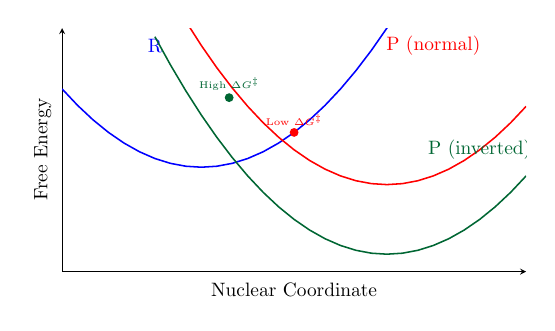
\begin{tikzpicture}[scale=0.7]
    \begin{axis}[
        xlabel={Nuclear Coordinate},
        ylabel={Free Energy},
        xtick=\empty, ytick=\empty,
        axis lines=left,
        width=10cm,
        height=6cm,
        ymin=-3, ymax=4
    ]
    % Reactant
    \addplot[blue, thick, domain=-0.5:3.5] {(x-1)^2};
    \node[blue] at (axis cs:0.5,3.5) {R};

    % Product (normal)
    \addplot[red, thick, domain=0.5:4.5] {(x-3)^2 - 0.5};
    \node[red] at (axis cs:3.5,3.5) {P (normal)};

    % Product (inverted)
    \addplot[darkgreen, thick, domain=0.5:4.5] {(x-3)^2 - 2.5};
    \node[darkgreen] at (axis cs:4,0.5) {P (inverted)};

    % Intersection points
    \fill[red] (axis cs:2,1) circle (0.08cm) node[above] {\tiny Low $\Delta G^\ddagger$};
    \fill[darkgreen] (axis cs:1.3,2) circle (0.08cm) node[above] {\tiny High $\Delta G^\ddagger$};
    \end{axis}
\end{tikzpicture}
\end{center}

In inverted region: Surfaces intersect at \alert{high energy} because product well is too far down.

\end{frame}

% ===========================================================================
% Slide: Experimental Evidence - Part 1
% ===========================================================================
\begin{frame}{Experimental Evidence for Inverted Region (Part 1)}

\textbf{Challenge:} Hard to observe - requires large $|\Delta_r G^\circ|$ while keeping $\lambda$ small.

\vspace{0.5cm}
\textbf{Early Evidence (Closs \& Miller, 1984):}
\begin{itemize}
    \item Intramolecular ET in rigid molecules
    \item Donor-Bridge-Acceptor systems
    \item Fixed distance, variable driving force
    \item Observed rate maximum and subsequent decrease
\end{itemize}

\vspace{0.5cm}
\textbf{Breakthrough:} First direct confirmation of Marcus inverted region

\end{frame}

% ===========================================================================
% Slide: Experimental Evidence - Part 2
% ===========================================================================
\begin{frame}{Experimental Evidence for Inverted Region (Part 2)}

\textbf{Modern Examples:}
\begin{itemize}
    \item Photoinduced back-electron transfer in donor-acceptor dyads
    \item Observed in porphyrin-quinone systems
    \item Common in photosynthetic reaction centers
    \item Used to slow down unproductive back-reactions
\end{itemize}

\vspace{0.5cm}
\textbf{Biological Significance:}
\begin{itemize}
    \item Nature uses inverted region to prevent energy-wasting back-transfer
    \item Essential for efficient energy conversion
    \item Protects high-energy charge-separated states
\end{itemize}

\end{frame}

% ===========================================================================
% Slide: Distance Dependence
% ===========================================================================
\begin{frame}{Distance Dependence of ET}

\textbf{Electronic Coupling:} Electron must \alert{tunnel} between D and A.

\keyeq{H_{DA} \propto \exp(-\beta r/2)}

where:
\begin{itemize}
    \item $H_{DA}$: Electronic coupling matrix element
    \item $r$: edge-to-edge distance
    \item $\beta$: decay parameter (depends on medium)
\end{itemize}

\vspace{0.3cm}
\textbf{Rate Dependence:}
\keyeq{k_{ET} \propto H_{DA}^2 \propto \exp(-\beta r)}

\vspace{0.3cm}
\textbf{Typical $\beta$ values:}
\begin{itemize}
    \item Vacuum/protein: $\beta \approx 16$-$20$ nm$^{-1}$ (fast decay)
    \item Through $\pi$-conjugated bridge: $\beta \approx 2$-$5$ nm$^{-1}$ (slow decay)
    \item Through $\sigma$ bonds: $\beta \approx 8$-$12$ nm$^{-1}$
\end{itemize}

\end{frame}

% ===========================================================================
% Slide: Semiclassical Marcus-Hush Theory - Part 1
% ===========================================================================
\begin{frame}{Semiclassical Marcus-Hush Theory (Part 1)}

\textbf{Full Expression:}

\keyeq{k_{ET} = \frac{2\pi}{\hbar}H_{DA}^2 \frac{1}{\sqrt{4\pi\lambda k_B T}} \exp\left(-\frac{(\Delta_r G^\circ + \lambda)^2}{4\lambda k_B T}\right)}

\vspace{0.5cm}
\textbf{This combines:}
\begin{itemize}
    \item Quantum mechanics (electron tunneling)
    \item Classical mechanics (nuclear reorganization)
    \item Statistical mechanics (thermal activation)
\end{itemize}

\end{frame}

% ===========================================================================
% Slide: Semiclassical Marcus-Hush Theory - Part 2
% ===========================================================================
\begin{frame}{Semiclassical Marcus-Hush Theory (Part 2)}

\textbf{Three Factors:}

\begin{enumerate}
    \item \textbf{Electronic Factor:} $H_{DA}^2$
        \begin{itemize}
            \item Tunneling probability
            \item Decreases exponentially with distance
        \end{itemize}

    \item \textbf{Nuclear Factor:} $\frac{1}{\sqrt{4\pi\lambda k_B T}}$
        \begin{itemize}
            \item Franck-Condon weighted density of states
            \item Pre-exponential factor
        \end{itemize}

    \item \textbf{Activation Factor:} $\exp\left(-\frac{(\Delta_r G^\circ + \lambda)^2}{4\lambda k_B T}\right)$
        \begin{itemize}
            \item Marcus activation energy
            \item Temperature dependent
        \end{itemize}
\end{enumerate}

\end{frame}

% ===========================================================================
% Slide: Marcus Cross Relation
% ===========================================================================
\begin{frame}{Marcus Cross Relation}

\textbf{Goal:} Predict rate of cross reaction from self-exchange rates.

For: \ch{D_1 + A_2 -> D_1^+ + A_2^-}

\keyeq{k_{12} = \sqrt{k_{11} k_{22} K_{12} f_{12}}}

where:
\begin{itemize}
    \item $k_{11}$: self-exchange rate of D$_1$/D$_1^+$
    \item $k_{22}$: self-exchange rate of A$_2$/A$_2^-$
    \item $K_{12}$: equilibrium constant = $\exp(-\Delta_r G^\circ / RT)$
    \item $f_{12}$: correction factor (usually $\approx 1$ for small $\Delta_r G^\circ$)
\end{itemize}

\vspace{0.3cm}
\textbf{Utility:}
\begin{itemize}
    \item Self-exchange rates are easier to measure
    \item Predict rates for many cross reactions
    \item Test consistency of Marcus theory
\end{itemize}

\end{frame}

% ===========================================================================
% Slide: Biological Electron Transfer - Part 1
% ===========================================================================
\begin{frame}{Biological Electron Transfer (Part 1)}

\textbf{Electron Transport Chains:}

\begin{itemize}
    \item \textbf{Photosynthesis:} P680 → Pheophytin → Q$_A$ → Q$_B$
    \item \textbf{Respiration:} NADH → Complex I → Q → Complex III → Cyt c → Complex IV → O$_2$
\end{itemize}

\vspace{0.5cm}
\textbf{Design Principles:}

\begin{enumerate}
    \item \textbf{Forward ET in Normal Region:}
        \begin{itemize}
            \item $-\Delta_r G^\circ < \lambda$ → fast forward transfer
        \end{itemize}

    \item \textbf{Back ET in Inverted Region:}
        \begin{itemize}
            \item $-\Delta_r G^\circ > \lambda$ → slow wasteful back-transfer
            \item Prevents energy loss
        \end{itemize}
\end{enumerate}

\end{frame}

% ===========================================================================
% Slide: Biological Electron Transfer - Part 2
% ===========================================================================
\begin{frame}{Biological Electron Transfer (Part 2)}

\textbf{Design Principles (continued):}

\begin{enumerate}
    \setcounter{enumi}{2}
    \item \textbf{Optimal Distances:}
        \begin{itemize}
            \item Typically 10-15 Å edge-to-edge
            \item Fast enough but selective
            \item Prevents short-circuits
        \end{itemize}

    \item \textbf{Protein Bridges:}
        \begin{itemize}
            \item Lower $\beta$ through aromatic residues
            \item Facilitate long-range transfer
            \item Guide electron path
        \end{itemize}
\end{enumerate}

\vspace{0.5cm}
\textbf{Result:} Efficient directional ET with minimal energy loss!

\end{frame}

% ===========================================================================
% Slide: Worked Example 1
% ===========================================================================
\begin{frame}{Worked Example 1: Calculating λ$_{\text{out}}$}

\textbf{Problem:} Calculate $\lambda_{\text{out}}$ for ET between two spherical ions with $r_D = r_A = 0.3$ nm separated by $d = 0.8$ nm in water ($\varepsilon_s = 80$, $n = 1.33$).

\vspace{0.3cm}
\textbf{Solution:}

\[ \lambda_{\text{out}} = \frac{e^2}{4\pi\varepsilon_0}\left(\frac{1}{2r_D} + \frac{1}{2r_A} - \frac{1}{d}\right)\left(\frac{1}{n^2} - \frac{1}{\varepsilon_s}\right) \]

Constants: $\frac{e^2}{4\pi\varepsilon_0} = 1.44$ eV·nm

\[ \lambda_{\text{out}} = 1.44 \left(\frac{1}{2(0.3)} + \frac{1}{2(0.3)} - \frac{1}{0.8}\right)\left(\frac{1}{1.77} - \frac{1}{80}\right) \]

\[ = 1.44(1.67 + 1.67 - 1.25)(0.565 - 0.0125) \]

\[ = 1.44(2.09)(0.553) = 1.66 \text{ eV} \]

\keyeq{\lambda_{\text{out}} = 1.66 \text{ eV} = 160 \text{ kJ/mol}}

\end{frame}

% ===========================================================================
% Slide: Worked Example 2
% ===========================================================================
\begin{frame}{Worked Example 2: Marcus Activation Energy}

\textbf{Problem:} For an ET reaction with $\lambda = 1.0$ eV and $\Delta_r G^\circ = -0.4$ eV, calculate:
\begin{enumerate}[a)]
    \item The activation energy $\Delta G^\ddagger$
    \item The rate constant at 298 K (assume $\nu_n = 10^{13}$ s$^{-1}$, $\kappa = 1$)
\end{enumerate}

\vspace{0.3cm}
\textbf{Solution:}

(a) Marcus equation:
\[ \Delta G^\ddagger = \frac{(\Delta_r G^\circ + \lambda)^2}{4\lambda} = \frac{(-0.4 + 1.0)^2}{4(1.0)} = \frac{(0.6)^2}{4} = 0.09 \text{ eV} \]

(b) Rate constant:
\[ k_{ET} = 10^{13} \exp\left(-\frac{0.09 \times 96.5}{8.314 \times 0.298}\right) = 10^{13} \exp(-3.50) \]
\[ = 10^{13} \times 0.030 = 3.0 \times 10^{11} \text{ s}^{-1} \]

\keyeq{k_{ET} = 3.0 \times 10^{11} \text{ s}^{-1}}

\textbf{Note:} Very fast! In normal region ($-\Delta_r G^\circ < \lambda$).

\end{frame}

% ===========================================================================
% Slide: Worked Example 3
% ===========================================================================
\begin{frame}{Worked Example 3: Inverted Region}

\textbf{Problem:} For the same system ($\lambda = 1.0$ eV), calculate $\Delta G^\ddagger$ for:
\begin{enumerate}[a)]
    \item $\Delta_r G^\circ = -1.0$ eV (barrierless)
    \item $\Delta_r G^\circ = -2.0$ eV (inverted)
\end{enumerate}

Compare with normal region ($\Delta_r G^\circ = -0.4$ eV, $\Delta G^\ddagger = 0.09$ eV).

\vspace{0.3cm}
\textbf{Solution:}

(a) Barrierless:
\[ \Delta G^\ddagger = \frac{(-1.0 + 1.0)^2}{4(1.0)} = 0 \text{ eV} \]

(b) Inverted:
\[ \Delta G^\ddagger = \frac{(-2.0 + 1.0)^2}{4(1.0)} = \frac{1.0}{4} = 0.25 \text{ eV} \]

\textbf{Trend:} $\Delta G^\ddagger = 0.09 \to 0 \to 0.25$ eV

Rate \alert{increases} then \alert{decreases} as $-\Delta_r G^\circ$ increases!

\end{frame}

% ===========================================================================
% Slide: Practice Problem 1
% ===========================================================================
\begin{frame}{Practice Problem 1}

\textbf{Problem:} An ET reaction has the following parameters:
\begin{itemize}
    \item $\lambda = 0.8$ eV
    \item $\Delta_r G^\circ = -0.6$ eV
    \item Distance: $r = 1.0$ nm
    \item $\beta = 10$ nm$^{-1}$
\end{itemize}

\begin{enumerate}[a)]
    \item Calculate $\Delta G^\ddagger$
    \item Is this in normal, barrierless, or inverted region?
    \item If distance increases to 1.5 nm, by what factor does rate decrease?
\end{enumerate}

\vspace{0.3cm}
\textbf{Answers:}
\begin{itemize}
    \item[(a)] $\Delta G^\ddagger = 0.01$ eV
    \item[(b)] Normal region ($-\Delta_r G^\circ < \lambda$)
    \item[(c)] Rate decreases by factor $\exp(\beta \Delta r) = \exp(10 \times 0.5) \approx 150$
\end{itemize}

\end{frame}

% ===========================================================================
% Slide: Practice Problem 2
% ===========================================================================
\begin{frame}{Practice Problem 2}

\textbf{Problem:} The self-exchange rate constants are:
\begin{itemize}
    \item \ch{Fe^{2+}/Fe^{3+}}: $k_{11} = 4.0$ M$^{-1}$s$^{-1}$
    \item \ch{Ru^{2+}/Ru^{3+}}: $k_{22} = 4.0 \times 10^2$ M$^{-1}$s$^{-1}$
\end{itemize}

For cross reaction \ch{Fe^{2+} + Ru^{3+} -> Fe^{3+} + Ru^{2+}}:
\begin{itemize}
    \item $\Delta_r G^\circ = -15$ kJ/mol
    \item $K_{12} = \exp(15000/(8.314 \times 298)) = 403$
\end{itemize}

Estimate $k_{12}$ using Marcus cross relation ($f_{12} \approx 1$).

\vspace{0.3cm}
\textbf{Solution:}
\[ k_{12} = \sqrt{k_{11} k_{22} K_{12}} = \sqrt{4.0 \times 400 \times 403} = \sqrt{6.4 \times 10^5} \]

\keyeq{k_{12} \approx 800 \text{ M}^{-1}\text{s}^{-1}}

\end{frame}

% ===========================================================================
% Slide: Practice Problem 3
% ===========================================================================
\begin{frame}{Practice Problem 3}

\textbf{Problem:} A biological ET chain has three steps:

\begin{center}
\begin{tabular}{ccc}
Step & $\Delta_r G^\circ$ (eV) & $\lambda$ (eV) \\
\hline
$1 \to 2$ & $-0.3$ & $0.8$ \\
$2 \to 3$ & $-0.5$ & $0.8$ \\
$3 \to 1$ (back) & $+0.8$ & $0.8$ \\
\end{tabular}
\end{center}

\begin{enumerate}[a)]
    \item Calculate $\Delta G^\ddagger$ for each step
    \item Which step is fastest?
    \item Why is the back-reaction slow despite being exergonic overall?
\end{enumerate}

\vspace{0.3cm}
\textbf{Answers:}
\begin{itemize}
    \item[(a)] $\Delta G^\ddagger(1\to2) = 0.078$ eV; $\Delta G^\ddagger(2\to3) = 0.028$ eV; $\Delta G^\ddagger(\text{back}) = 0.2$ eV
    \item[(b)] Step $2 \to 3$ (lowest barrier)
    \item[(c)] Back-reaction has endergonic $\Delta_r G^\circ$, creating large barrier
\end{itemize}

\end{frame}

% ===========================================================================
% Slide: Practice Problem 4
% ===========================================================================
\begin{frame}{Practice Problem 4}

\textbf{Problem:} For optimal ET rate (barrierless), we need $-\Delta_r G^\circ = \lambda$.

A photosynthetic reaction center has:
\begin{itemize}
    \item Forward ET: $\lambda = 0.5$ eV
    \item Back ET: $\lambda = 0.5$ eV
\end{itemize}

\begin{enumerate}[a)]
    \item What driving force gives fastest forward ET?
    \item If actual $\Delta_r G^\circ = -0.3$ eV, what is $\Delta G^\ddagger$?
    \item For back ET with $\Delta_r G^\circ = +0.3$ eV, what is the barrier?
    \item How does this design prevent energy loss?
\end{enumerate}

\vspace{0.3cm}
\textbf{Answers:}
\begin{itemize}
    \item[(a)] $\Delta_r G^\circ = -0.5$ eV (= $-\lambda$)
    \item[(b)] $\Delta G^\ddagger = 0.02$ eV (fast)
    \item[(c)] $\Delta G^\ddagger = 0.32$ eV (slow!)
    \item[(d)] Endergonic back-reaction has huge barrier → prevents wasteful back-transfer
\end{itemize}

\end{frame}

% ===========================================================================
% Slide: Summary Topic 18E
% ===========================================================================
\begin{frame}{Summary: Topic 18E}

\begin{enumerate}
    \item \textbf{Franck-Condon Principle:} ET is vertical transition at fixed nuclear geometry
    \[ \text{Time}_{\text{electron}} \ll \text{Time}_{\text{nuclear}} \]

    \item \textbf{Reorganization Energy:} $\lambda = \lambda_{\text{in}} + \lambda_{\text{out}}$
        \begin{itemize}
            \item Cost to rearrange nuclei before ET
        \end{itemize}

    \item \textbf{Marcus Equation:}
    \[ \Delta G^\ddagger = \frac{(\Delta_r G^\circ + \lambda)^2}{4\lambda} \]
        \begin{itemize}
            \item Normal region: rate increases with $-\Delta_r G^\circ$
            \item Barrierless: $-\Delta_r G^\circ = \lambda$ (maximum rate)
            \item Inverted region: rate decreases with $-\Delta_r G^\circ$
        \end{itemize}

    \item \textbf{Distance Dependence:} $k_{ET} \propto \exp(-\beta r)$
        \begin{itemize}
            \item Electron tunneling through barrier
        \end{itemize}

    \item \textbf{Biological Applications:} Optimized ET chains use normal + inverted regions
\end{enumerate}

\end{frame}

% ===========================================================================
% Slide: Interactive Resources for Topic 18E
% ===========================================================================
\begin{frame}{Interactive Learning: Topic 18E}

\begin{columns}[c]
\column{0.65\textwidth}
\textbf{Explore Electron Transfer Theory Interactively!}

\vspace{0.3cm}

\textbf{Interactive Jupyter Notebook Features:}
\begin{itemize}
    \item \textbf{Marcus Parabola Explorer}: Visualize normal, barrierless, inverted
    \item \textbf{Reorganization Energy Calculator}: Inner + outer sphere
    \item \textbf{Driving Force vs Rate}: Interactive $k$ vs $-\Delta_r G^\circ$ plots
    \item \textbf{Tunneling Distance Decay}: Exponential $\beta$ dependence
    \item \textbf{Biological ET Chains}: Photosynthesis, respiration
    \item \textbf{Real Systems}: Ru complexes, cytochrome c
\end{itemize}

\vspace{0.3cm}

\textbf{Notebook:} \texttt{05\_Electron\_Transfer.ipynb}

\column{0.35\textwidth}
\centering
\textbf{Scan to Open:}

\vspace{0.3cm}

\includegraphics[width=0.8\textwidth]{QR_codes/05_Electron_Transfer.png}

\vspace{0.3cm}

{\footnotesize Or navigate to:\\
\texttt{Reaction\_Dynamics\_Interactive/}}

\end{columns}

\end{frame}



% ============================================================================
% SUMMARY
% ============================================================================
\section{Summary and Conclusions}

\begin{frame}{Comparison of Theories}

\small
\begin{table}
\centering
\begin{tabular}{lcccc}
\toprule
\textbf{Theory} & \textbf{Collision} & \textbf{Diffusion} & \textbf{TST} & \textbf{Marcus} \\
\midrule
Phase & Gas & Liquid & All & All \\
\addlinespace
Key parameter & $\sigma$, $E_a$ & $D$, $\eta$ & $\Delta^{\ddagger} G^{\circ}$ & $\lambda$ \\
\addlinespace
Rate equation & $\sigma v e^{-E_a/RT}$ & $4\pi RD$ & $\frac{kT}{h}e^{-\Delta G^{\ddagger}/RT}$ & $|H_{AB}|^2 e^{-\Delta G^{\ddagger}/RT}$ \\
\addlinespace
Entropy? & No & No & \textbf{Yes} & \textbf{Yes} \\
\addlinespace
Quantum? & No & No & Limited & \textbf{Yes} \\
\addlinespace
Best for & Simple gas rxns & Fast rxns & General & ET \\
\bottomrule
\end{tabular}
\end{table}
\normalsize

\vspace{0.3cm}

\emphbox{Each theory has its domain of applicability}

\end{frame}

\begin{frame}{Common Themes}

\textbf{Throughout Focus 18:}

\vspace{0.3cm}

\begin{enumerate}
\item \textbf{Energy matters}
\begin{itemize}
\item Activation barriers control rates
\item Energy distribution among modes
\item Quantum vs. classical regimes
\end{itemize}

\vspace{0.2cm}

\item \textbf{Geometry matters}
\begin{itemize}
\item Molecular orientation (steric factors)
\item Potential energy surfaces
\item Reaction paths
\end{itemize}

\vspace{0.2cm}

\item \textbf{Potential energy surfaces}
\begin{itemize}
\item Central concept in all theories
\item Saddle points = transition states
\item Guide reaction dynamics
\end{itemize}

\vspace{0.2cm}

\item \textbf{Quantum effects}
\begin{itemize}
\item Tunneling (H-transfer, ET)
\item Zero-point energy (KIE)
\item Electronic coupling
\end{itemize}
\end{enumerate}

\end{frame}

\begin{frame}{Applications}

\textbf{Reaction dynamics principles apply to:}

\vspace{0.3cm}

\begin{columns}[T]

\column{0.5\textwidth}

\textbf{Atmospheric Chemistry:}
\begin{itemize}
\item Ozone formation/depletion
\item Radical reactions
\item Aerosol chemistry
\end{itemize}

\vspace{0.3cm}

\textbf{Combustion:}
\begin{itemize}
\item Flame chemistry
\item Explosions
\item Engine efficiency
\end{itemize}

\vspace{0.3cm}

\textbf{Materials Science:}
\begin{itemize}
\item Surface reactions
\item Catalysis
\item Corrosion
\end{itemize}

\column{0.5\textwidth}

\textbf{Biochemistry:}
\begin{itemize}
\item Enzyme mechanisms
\item Electron transport chains
\item Photosynthesis
\end{itemize}

\vspace{0.3cm}

\textbf{Energy Conversion:}
\begin{itemize}
\item Solar cells
\item Batteries
\item Fuel cells
\end{itemize}

\vspace{0.3cm}

\textbf{Pharmaceuticals:}
\begin{itemize}
\item Drug design
\item Reaction optimization
\item Metabolic pathways
\end{itemize}

\end{columns}

\end{frame}

\begin{frame}{Further Resources}

\textbf{Recommended Reading:}

\begin{itemize}
\item Atkins \& de Paula: \textit{Physical Chemistry}, Chapter 18
\item Steinfeld, Francisco \& Hase: \textit{Chemical Kinetics and Dynamics}
\item Levine: \textit{Molecular Reaction Dynamics}
\item Marcus: Nobel Lecture (1992) on electron transfer
\end{itemize}

\vspace{0.3cm}

\textbf{Interactive Resources:}

\begin{itemize}
\item Jupyter notebooks for each topic (see QR codes throughout)
\item PhET simulations: Collision theory, reaction dynamics
\item Computational chemistry software: Gaussian, ORCA, Q-Chem
\end{itemize}

\vspace{0.3cm}

\textbf{Advanced Topics:}

\begin{itemize}
\item Femtochemistry (Nobel Prize 1999 - Ahmed Zewail)
\item Attosecond science
\item Machine learning potentials
\item Quantum control of reactions
\end{itemize}

\end{frame}

% ============================================================================
% FINAL SLIDE
% ============================================================================
\begin{frame}[plain]

\begin{center}
{\Huge Questions?}

\vspace{1cm}

{\Large Thank you for your attention!}

\vspace{1cm}

\textit{From simple collisions to complex electron transfer,\\
reaction dynamics reveals the beauty of chemistry at the molecular level}

\end{center}

\end{frame}

\end{document}
